% Options for packages loaded elsewhere
\PassOptionsToPackage{unicode}{hyperref}
\PassOptionsToPackage{hyphens}{url}
%
\documentclass[
]{book}
\usepackage{amsmath,amssymb}
\usepackage{iftex}
\ifPDFTeX
  \usepackage[T1]{fontenc}
  \usepackage[utf8]{inputenc}
  \usepackage{textcomp} % provide euro and other symbols
\else % if luatex or xetex
  \usepackage{unicode-math} % this also loads fontspec
  \defaultfontfeatures{Scale=MatchLowercase}
  \defaultfontfeatures[\rmfamily]{Ligatures=TeX,Scale=1}
\fi
\usepackage{lmodern}
\ifPDFTeX\else
  % xetex/luatex font selection
\fi
% Use upquote if available, for straight quotes in verbatim environments
\IfFileExists{upquote.sty}{\usepackage{upquote}}{}
\IfFileExists{microtype.sty}{% use microtype if available
  \usepackage[]{microtype}
  \UseMicrotypeSet[protrusion]{basicmath} % disable protrusion for tt fonts
}{}
\makeatletter
\@ifundefined{KOMAClassName}{% if non-KOMA class
  \IfFileExists{parskip.sty}{%
    \usepackage{parskip}
  }{% else
    \setlength{\parindent}{0pt}
    \setlength{\parskip}{6pt plus 2pt minus 1pt}}
}{% if KOMA class
  \KOMAoptions{parskip=half}}
\makeatother
\usepackage{xcolor}
\usepackage{color}
\usepackage{fancyvrb}
\newcommand{\VerbBar}{|}
\newcommand{\VERB}{\Verb[commandchars=\\\{\}]}
\DefineVerbatimEnvironment{Highlighting}{Verbatim}{commandchars=\\\{\}}
% Add ',fontsize=\small' for more characters per line
\usepackage{framed}
\definecolor{shadecolor}{RGB}{248,248,248}
\newenvironment{Shaded}{\begin{snugshade}}{\end{snugshade}}
\newcommand{\AlertTok}[1]{\textcolor[rgb]{0.94,0.16,0.16}{#1}}
\newcommand{\AnnotationTok}[1]{\textcolor[rgb]{0.56,0.35,0.01}{\textbf{\textit{#1}}}}
\newcommand{\AttributeTok}[1]{\textcolor[rgb]{0.13,0.29,0.53}{#1}}
\newcommand{\BaseNTok}[1]{\textcolor[rgb]{0.00,0.00,0.81}{#1}}
\newcommand{\BuiltInTok}[1]{#1}
\newcommand{\CharTok}[1]{\textcolor[rgb]{0.31,0.60,0.02}{#1}}
\newcommand{\CommentTok}[1]{\textcolor[rgb]{0.56,0.35,0.01}{\textit{#1}}}
\newcommand{\CommentVarTok}[1]{\textcolor[rgb]{0.56,0.35,0.01}{\textbf{\textit{#1}}}}
\newcommand{\ConstantTok}[1]{\textcolor[rgb]{0.56,0.35,0.01}{#1}}
\newcommand{\ControlFlowTok}[1]{\textcolor[rgb]{0.13,0.29,0.53}{\textbf{#1}}}
\newcommand{\DataTypeTok}[1]{\textcolor[rgb]{0.13,0.29,0.53}{#1}}
\newcommand{\DecValTok}[1]{\textcolor[rgb]{0.00,0.00,0.81}{#1}}
\newcommand{\DocumentationTok}[1]{\textcolor[rgb]{0.56,0.35,0.01}{\textbf{\textit{#1}}}}
\newcommand{\ErrorTok}[1]{\textcolor[rgb]{0.64,0.00,0.00}{\textbf{#1}}}
\newcommand{\ExtensionTok}[1]{#1}
\newcommand{\FloatTok}[1]{\textcolor[rgb]{0.00,0.00,0.81}{#1}}
\newcommand{\FunctionTok}[1]{\textcolor[rgb]{0.13,0.29,0.53}{\textbf{#1}}}
\newcommand{\ImportTok}[1]{#1}
\newcommand{\InformationTok}[1]{\textcolor[rgb]{0.56,0.35,0.01}{\textbf{\textit{#1}}}}
\newcommand{\KeywordTok}[1]{\textcolor[rgb]{0.13,0.29,0.53}{\textbf{#1}}}
\newcommand{\NormalTok}[1]{#1}
\newcommand{\OperatorTok}[1]{\textcolor[rgb]{0.81,0.36,0.00}{\textbf{#1}}}
\newcommand{\OtherTok}[1]{\textcolor[rgb]{0.56,0.35,0.01}{#1}}
\newcommand{\PreprocessorTok}[1]{\textcolor[rgb]{0.56,0.35,0.01}{\textit{#1}}}
\newcommand{\RegionMarkerTok}[1]{#1}
\newcommand{\SpecialCharTok}[1]{\textcolor[rgb]{0.81,0.36,0.00}{\textbf{#1}}}
\newcommand{\SpecialStringTok}[1]{\textcolor[rgb]{0.31,0.60,0.02}{#1}}
\newcommand{\StringTok}[1]{\textcolor[rgb]{0.31,0.60,0.02}{#1}}
\newcommand{\VariableTok}[1]{\textcolor[rgb]{0.00,0.00,0.00}{#1}}
\newcommand{\VerbatimStringTok}[1]{\textcolor[rgb]{0.31,0.60,0.02}{#1}}
\newcommand{\WarningTok}[1]{\textcolor[rgb]{0.56,0.35,0.01}{\textbf{\textit{#1}}}}
\usepackage{longtable,booktabs,array}
\usepackage{calc} % for calculating minipage widths
% Correct order of tables after \paragraph or \subparagraph
\usepackage{etoolbox}
\makeatletter
\patchcmd\longtable{\par}{\if@noskipsec\mbox{}\fi\par}{}{}
\makeatother
% Allow footnotes in longtable head/foot
\IfFileExists{footnotehyper.sty}{\usepackage{footnotehyper}}{\usepackage{footnote}}
\makesavenoteenv{longtable}
\usepackage{graphicx}
\makeatletter
\def\maxwidth{\ifdim\Gin@nat@width>\linewidth\linewidth\else\Gin@nat@width\fi}
\def\maxheight{\ifdim\Gin@nat@height>\textheight\textheight\else\Gin@nat@height\fi}
\makeatother
% Scale images if necessary, so that they will not overflow the page
% margins by default, and it is still possible to overwrite the defaults
% using explicit options in \includegraphics[width, height, ...]{}
\setkeys{Gin}{width=\maxwidth,height=\maxheight,keepaspectratio}
% Set default figure placement to htbp
\makeatletter
\def\fps@figure{htbp}
\makeatother
\setlength{\emergencystretch}{3em} % prevent overfull lines
\providecommand{\tightlist}{%
  \setlength{\itemsep}{0pt}\setlength{\parskip}{0pt}}
\setcounter{secnumdepth}{5}
\usepackage{booktabs}
\usepackage{amsthm}
\makeatletter
\def\thm@space@setup{%
  \thm@preskip=8pt plus 2pt minus 4pt
  \thm@postskip=\thm@preskip
}
\makeatother
\usepackage{booktabs}
\usepackage{longtable}
\usepackage{array}
\usepackage{multirow}
\usepackage{wrapfig}
\usepackage{float}
\usepackage{colortbl}
\usepackage{pdflscape}
\usepackage{tabu}
\usepackage{threeparttable}
\usepackage{threeparttablex}
\usepackage[normalem]{ulem}
\usepackage{makecell}
\usepackage{xcolor}
\ifLuaTeX
  \usepackage{selnolig}  % disable illegal ligatures
\fi
\usepackage[]{natbib}
\bibliographystyle{apalike}
\usepackage{bookmark}
\IfFileExists{xurl.sty}{\usepackage{xurl}}{} % add URL line breaks if available
\urlstyle{same}
\hypersetup{
  pdftitle={EUR/USD},
  pdfauthor={Harvey Bastidas, Andrés Caicedo, Alexander Alvarado},
  hidelinks,
  pdfcreator={LaTeX via pandoc}}

\title{EUR/USD}
\author{Harvey Bastidas, Andrés Caicedo, Alexander Alvarado}
\date{2024-11-29}

\begin{document}
\maketitle

{
\setcounter{tocdepth}{1}
\tableofcontents
}
\chapter{Justificación de elección del Dataset}\label{justificaciuxf3n-de-elecciuxf3n-del-dataset}

\textbf{Integrantes}:\\
Harvey Bastidas, Alexander Alvarado y Andrés Caicedo\\
\textbf{Materia}:\\
Análisis de series de tiempo\\
\textbf{Profesora}:\\
Isabel Cristina García

\begin{center}\rule{0.5\linewidth}{0.5pt}\end{center}

\section{Información del Dataset}\label{informaciuxf3n-del-dataset}

El dataset seleccionado para este análisis es el siguiente: \href{https://www.kaggle.com/datasets/chandrimad31/eurusd-forex-trading-data-20032021}{EUR/USD Forex Trading Data (2003-2021)}, el cual fue extraído de \href{https://forex.tradingcharts.com/}{Forex Trading Charts}, propiedad de Barchart Solutions, una empresa especializada en servicios financieros en los Estados Unidos. Barchart Solutions cuenta con reconocidos clientes como el Banco Goldman Sachs y el Bank of Canada, lo que nos lleva a concluir que los datos ofrecidos son confiables y precisos para realizar análisis financieros.

La empresa matriz, \textbf{Barchart Solutions}, tiene su sede en:

\textbf{222 S. Riverside Plaza, Suite 810,\\
Chicago, IL 60606, Estados Unidos}

El dataset presenta las tasas de cambio del par de divisas EUR/USD desde el \textbf{5 de mayo de 2003} hasta el \textbf{16 de octubre de 2021}, con una periodicidad de \textbf{4 horas}. Este conjunto de datos incluye las siguientes 6 columnas:

\begin{itemize}
\tightlist
\item
  \textbf{Open}: Precio de apertura para el periodo.
\item
  \textbf{High}: Precio máximo durante el periodo.
\item
  \textbf{Low}: Precio mínimo durante el periodo.
\item
  \textbf{Close}: Precio de cierre para el periodo.
\item
  \textbf{Volume}: Volumen de transacciones reportado.
\end{itemize}

Es importante resaltar que los datos no contienen valores nulos ni perdidos para los días de semana, aunque no se registran valores durante los fines de semana, lo que es normal en los mercados de Forex.

El análisis se centrará en la columna \textbf{Close}, que representa el precio de cierre, dado que es la variable más relevante para el pronóstico de tendencias.

\section{Justificación de la Elección del Dataset}\label{justificaciuxf3n-de-la-elecciuxf3n-del-dataset}

La elección de este dataset se fundamenta en la importancia de analizar la tasa de cambio EUR/USD, uno de los pares de divisas más negociados en el mercado Forex. La predicción de la tendencia de la tasa de cambio es crucial para varias estrategias financieras, como el balanceo de portafolios de inversión. En este contexto, se pueden usar tanto la \textbf{Teoría Moderna de Portafolios (MPT)} como la \textbf{Teoría de Portafolios Post-Moderna (PMPT)}, que son ampliamente utilizadas en la optimización de la distribución de activos. Ambas teorías se benefician de predicciones precisas de la tendencia de los activos subyacentes, como es el caso de las divisas.

Además, este dataset ofrece una excelente relación señal-ruido, lo que mejora la predictibilidad de los modelos basados en series de tiempo. Utilizamos el \textbf{coeficiente de variación (CV)} como criterio para seleccionar este dataset, debido a que es una métrica robusta para medir la variabilidad en relación con la media. Un CV bajo indica que la variabilidad en los datos es relativamente baja, lo que es favorable para la predicción de tendencias.

El \textbf{coeficiente de variación} calculado para la columna ``Close'' de este dataset es de aproximadamente \textbf{9.5\%}, lo que lo convierte en el más bajo entre los datasets que evaluamos. Esto lo hace ideal para el pronóstico, ya que un CV bajo sugiere que la señal en los datos es fuerte en comparación con el ruido.

\subsection{Relación con el Signal-to-Noise Ratio (SNR)}\label{relaciuxf3n-con-el-signal-to-noise-ratio-snr}

El \textbf{coeficiente de variación (CV)} está inversamente relacionado con el \textbf{Signal-to-Noise Ratio (SNR)}, una métrica comúnmente utilizada en el procesamiento de señales. El SNR mide la proporción de la potencia de la señal con respecto a la del ruido, lo que ayuda a evaluar la calidad de los datos.

El SNR para este dataset se calcula como el cuadrado del inverso del CV. Para el EUR/USD, con un CV de \textbf{0.09}, el SNR es aproximadamente:

\[
SNR = \left(\frac{1}{0.09}\right)^2 \approx 123
\]

Este valor indica que la señal es mucho más fuerte que el ruido en este dataset. En contraste, otro dataset que probamos, con un CV de \textbf{20\%}, tenía un SNR mucho menor, alrededor de \textbf{25}. La diferencia muestra que el dataset de EUR/USD tiene una mayor preponderancia de señal sobre el ruido, lo que permite una mejor predictibilidad en los modelos de pronóstico.

Dado que sabemos que el \textbf{SNR} es aprox \textbf{123}, esto significa que el ruido es aprox 1/123 = \textbf{0.008} que nos da una idea del máximo error absoluto (\textbf{MAE}) en los datos Normalizados en el pronósitco del siguiente periodo que podemos obtener, ya que errores por debajo de este valor probablemente incluirían la predicción del ruido y podrían ser indicador de overfitting en el modelo predictivo usado.

\section{Importancia de Analizar este Dataset}\label{importancia-de-analizar-este-dataset}

La capacidad de predecir con precisión la tasa de cambio EUR/USD tiene múltiples aplicaciones en el sector financiero. En primer lugar, es fundamental para el \textbf{trading de divisas (Forex)}, donde una mejor predicción de las tendencias puede resultar en decisiones de inversión más acertadas. Además, es esencial para la gestión de portafolios financieros, ya que permite el uso de herramientas como la \textbf{Teoría Moderna de Portafolios (MPT)}, donde la diversificación se realiza teniendo en cuenta tanto la tendencia como la variabilidad de los activos.

Por lo tanto, este dataset fue seleccionado debido a su alta calidad y baja variabilidad, lo que lo hace ideal para el análisis predictivo en el mercado de Forex, así como en la gestión de portafolios. El alto \textbf{SNR} nos da confianza en que las predicciones basadas en este dataset serán precisas y útiles en un entorno real, al mismo tiempo que nos alerta sobre los límites predictivos en función del ruido presente en los datos.

\chapter{Estructura de los datos}\label{intro}

Con el propósito de observar las tendencias y cambios estructurales en la serie, se realizan pruebas estadísticas para conocer la estructura subyacente de la serie.

\section{Cálculo de Medias Móviles Simples:}\label{cuxe1lculo-de-medias-muxf3viles-simples}

El cálculo de medias móviles es una técnica común en el análisis de series de tiempo utilizada para suavizar las fluctuaciones a corto plazo y destacar las tendencias subyacentes en los datos. En este análisis, se implementan medias móviles de corto y largo plazo para identificar patrones de comportamiento y ayudar en la toma de decisiones basadas en tendencias más claras.

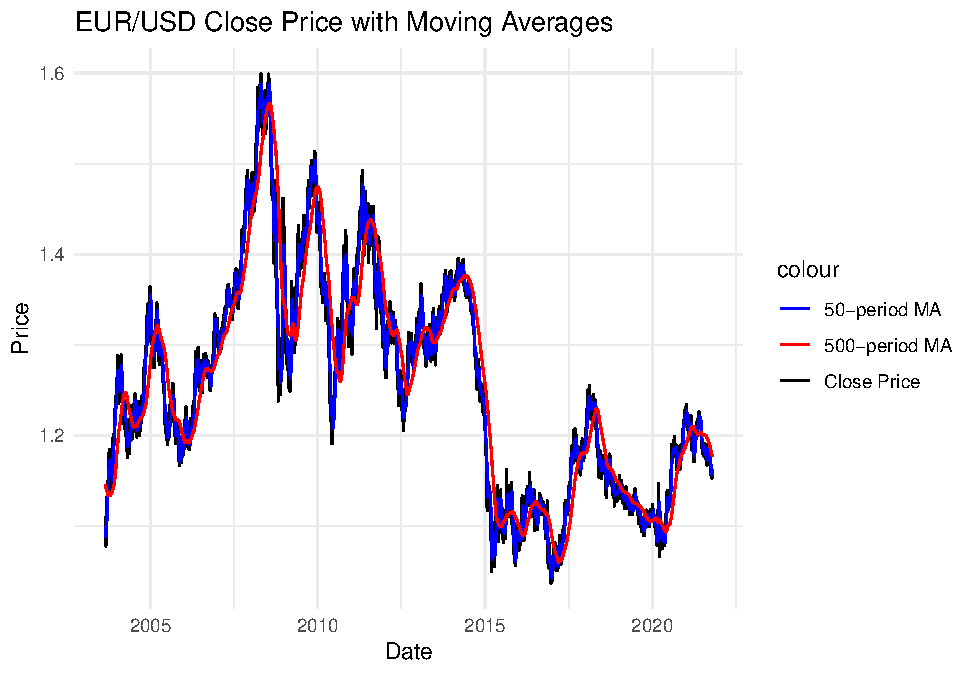
\includegraphics{bookdown_time_series_files/figure-latex/unnamed-chunk-3-1.pdf}

\begin{itemize}
\item
  \textbf{Media móvil de 50 periodos (MA corta)}:

  \begin{itemize}
  \item
    Sigue de cerca las fluctuaciones del precio de cierre, respondiendo rápidamente a los cambios de tendencia.
  \item
    Captura las tendencias a \textbf{corto plazo}, pero también refleja mucha volatilidad.
  \end{itemize}
\item
  \textbf{Media móvil de 500 periodos (MA larga)}:

  \begin{itemize}
  \item
    Se mueve de forma más suave, reaccionando más lentamente a los cambios de precios.
  \item
    Indica la \textbf{tendencia a largo plazo}, proporcionando una visión más estable del comportamiento del mercado.
  \end{itemize}
\end{itemize}

\section{Análisis de Rezagos}\label{anuxe1lisis-de-rezagos}

Cómo se comporta la serie de tiempo con respecto a sus valores pasados, introduciendo rezagos.

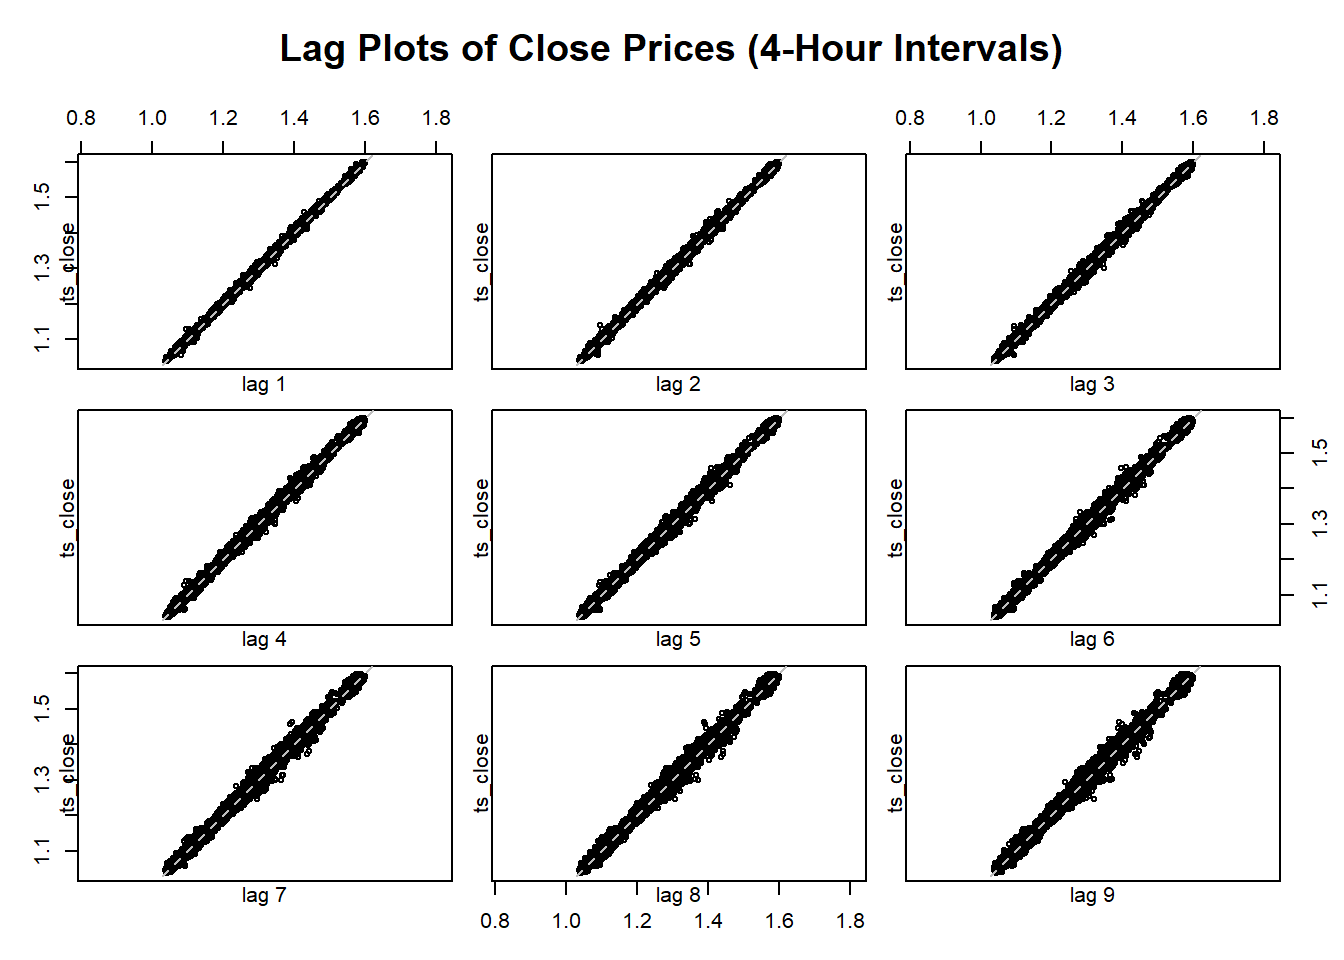
\includegraphics{bookdown_time_series_files/figure-latex/unnamed-chunk-5-1.pdf}

En cada uno de los gráficos, los puntos siguen una línea casi perfectamente recta, sugiriendo una \textbf{alta autocorrelación} entre los valores de la serie con sus rezagos cercanos.

La pendiente positiva indica que cuando el valor anterior era alto, el valor actual también tiende a ser alto, y lo mismo sucede para valores bajos. Esto sugiere que \textbf{la serie es muy persistente}, es decir, los precios tienden a seguir una dirección similar en el corto plazo.

Dado que no hay patrones dispersos o sin forma definida, se puede inferir que la serie no tiene cambios abruptos o comportamiento caótico entre los puntos cercanos. Esto podría indicar que \textbf{no hay mucha volatilidad} en los intervalos de 4 horas.

\section{Análisis de Estacionalidad}\label{anuxe1lisis-de-estacionalidad}

Para detectar si existe estacionalidad (patrones repetitivos), utilizaremos \textbf{decomposición} o \textbf{test de estacionalidad}.

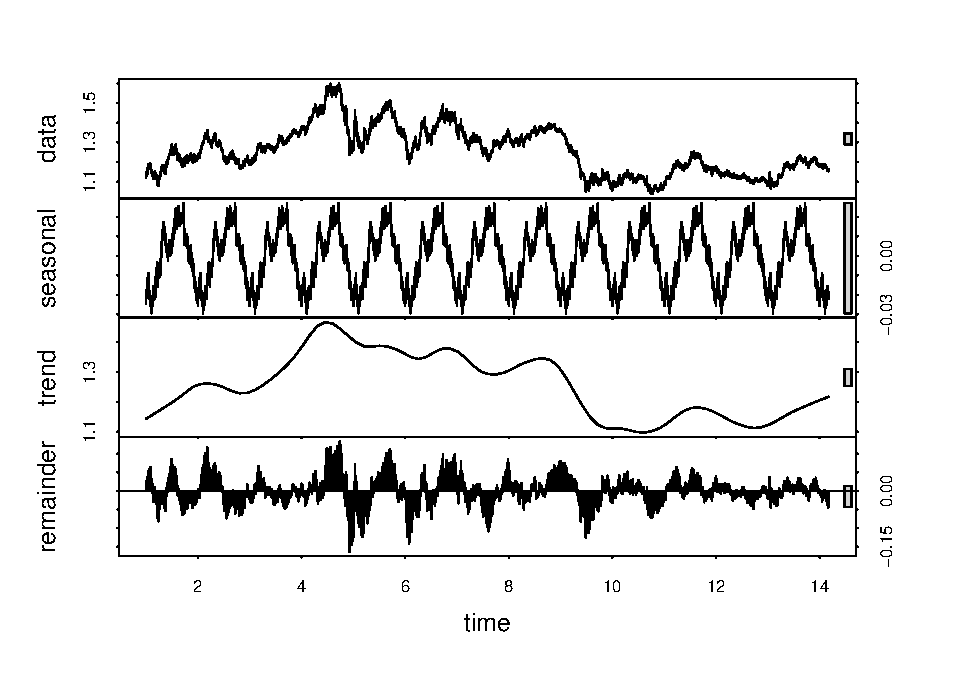
\includegraphics{bookdown_time_series_files/figure-latex/unnamed-chunk-6-1.pdf}

En la gráfica de \textbf{descomposición de series de tiempo} se visualizan los \textbf{componentes de la serie}: datos originales, estacionalidad, tendencia y residuales (remainder):

1. \textbf{Datos Originales (data):} En la primera gráfica (data), se observan los valores de cierre a lo largo del tiempo. Vemos fluctuaciones en los precios con algunas subidas y bajadas claras, lo que indica la volatilidad normal del mercado Forex.

2. \textbf{Componente Estacional (seasonal):} El segundo gráfico muestra un \textbf{patrón repetitivo y periódico}. Este patrón sugiere que hay \textbf{ciclos regulares} en la serie. La estacionalidad se mantiene constante a lo largo del tiempo, lo que indica que ciertos movimientos en el mercado se repiten con una periodicidad fija (en este caso, podría ser diaria o semanal). Es probable que este componente estacional refleje la actividad cíclica en horarios específicos o días determinados, como mayor volatilidad durante sesiones overlap (como entre Londres y Nueva York).

3. \textbf{Componente de Tendencia (trend):} El tercer gráfico muestra una \textbf{tendencia suavizada} que sigue la dirección general del mercado. Observamos fases de \textbf{alzas y caídas}: primero hay una subida clara, luego una caída, y finalmente otra leve tendencia hacia la estabilidad.

4. \textbf{Componente de Residuos o Resto (remainder):} El último gráfico (remainder) muestra los \textbf{residuos} o la parte de los datos que no es explicada por la tendencia ni la estacionalidad. Estos residuos parecen ser \textbf{ruido blanco}, con fluctuaciones alrededor de cero, lo que indica que no hay patrones significativos adicionales no capturados por los otros componentes.

\chapter{Preprocesamiento y Visualización}\label{preprocesamiento-y-visualizaciuxf3n}

En este análisis, trabajaremos con el dataset de tipo de cambio EUR/USD de Forex proporcionado, el cual incluye datos históricos de 2003 a 2021. El objetivo es estudiar las tendencias, estacionalidad y comportamiento estructural de la serie de tiempo. Además, evaluaremos si es necesario realizar transformaciones en la serie para estabilizar la varianza y facilitar la predicción.

\section{Descomposición de la Serie de Tiempo}\label{descomposiciuxf3n-de-la-serie-de-tiempo}

En esta etapa se busca realizar la descomposición de la serie de tiempo para identificar los componentes de \textbf{tendencia}, \textbf{estacionalidad} y \textbf{residuos}.

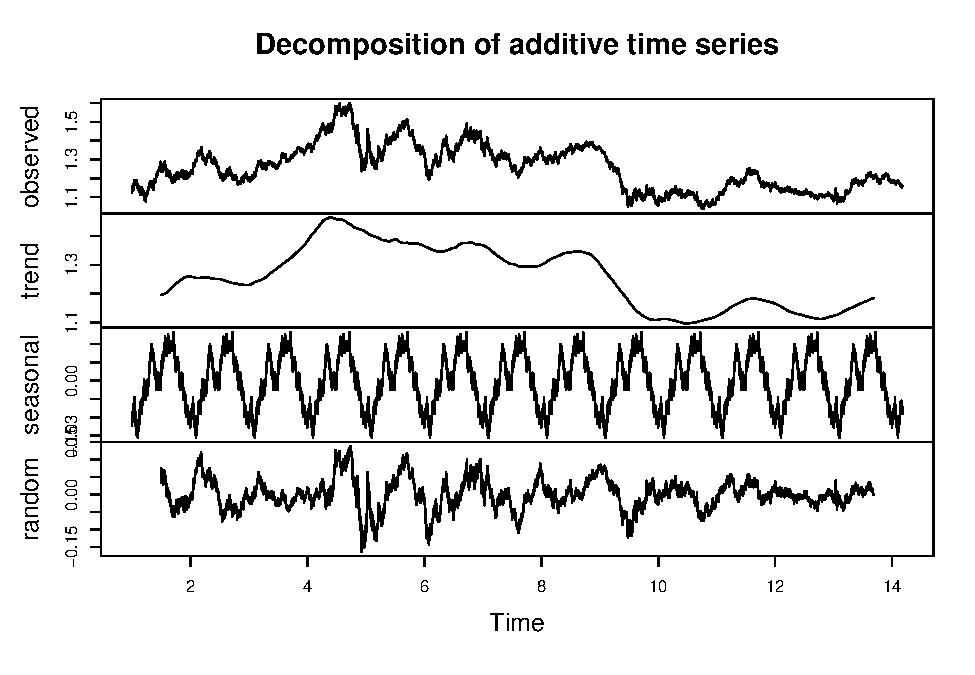
\includegraphics{bookdown_time_series_files/figure-latex/unnamed-chunk-8-1.pdf}

En la gráfica de \textbf{descomposición de series de tiempo} se visualizan los \textbf{componentes de la serie}: datos originales, estacionalidad, tendencia y residuales (remainder):

1. \textbf{Datos Originales (data):} En la primera gráfica (data), se observan los valores de cierre a lo largo del tiempo. Vemos fluctuaciones en los precios con algunas subidas y bajadas claras, lo que indica la volatilidad normal del mercado Forex.

2. \textbf{Componente Estacional (seasonal):} El segundo gráfico muestra un \textbf{patrón repetitivo y periódico}. Este patrón sugiere que hay \textbf{ciclos regulares} en la serie. La estacionalidad se mantiene constante a lo largo del tiempo, lo que indica que ciertos movimientos en el mercado se repiten con una periodicidad fija (en este caso, podría ser diaria o semanal). Es probable que este componente estacional refleje la actividad cíclica en horarios específicos o días determinados, como mayor volatilidad durante sesiones overlap (como entre Londres y Nueva York).

3. \textbf{Componente de Tendencia (trend):} El tercer gráfico muestra una \textbf{tendencia suavizada} que sigue la dirección general del mercado. Observamos fases de \textbf{alzas y caídas}: primero hay una subida clara, luego una caída, y finalmente otra leve tendencia hacia la estabilidad.

4. \textbf{Componente de Residuos o Resto (remainder):} El último gráfico (remainder) muestra los \textbf{residuos} o la parte de los datos que no es explicada por la tendencia ni la estacionalidad. Estos residuos parecen ser \textbf{ruido blanco}, con fluctuaciones alrededor de cero, lo que indica que no hay patrones significativos adicionales no capturados por los otros componentes.

\section{Prueba de Estacionariedad}\label{prueba-de-estacionariedad}

La estacionariedad es importante en el análisis de series de tiempo porque indica si las propiedades estadísticas de la serie (como la media y la varianza) se mantienen constantes a lo largo del tiempo. Una serie estacionaria es generalmente más fácil de modelar y predecir.

\begin{verbatim}
## Augmented Dickey-Fuller Test 
## alternative: stationary 
##  
## Type 1: no drift no trend 
##       lag    ADF p.value
##  [1,]   0 -0.135   0.606
##  [2,]   1 -0.133   0.606
##  [3,]   2 -0.135   0.606
##  [4,]   3 -0.131   0.607
##  [5,]   4 -0.143   0.603
##  [6,]   5 -0.146   0.603
##  [7,]   6 -0.149   0.602
##  [8,]   7 -0.147   0.602
##  [9,]   8 -0.155   0.600
## [10,]   9 -0.156   0.600
## [11,]  10 -0.158   0.599
## [12,]  11 -0.174   0.594
## [13,]  12 -0.172   0.595
## [14,]  13 -0.169   0.596
## [15,]  14 -0.166   0.597
## Type 2: with drift no trend 
##       lag   ADF p.value
##  [1,]   0 -2.20   0.248
##  [2,]   1 -2.21   0.244
##  [3,]   2 -2.23   0.238
##  [4,]   3 -2.19   0.253
##  [5,]   4 -2.20   0.250
##  [6,]   5 -2.20   0.248
##  [7,]   6 -2.21   0.244
##  [8,]   7 -2.20   0.248
##  [9,]   8 -2.19   0.254
## [10,]   9 -2.18   0.257
## [11,]  10 -2.18   0.255
## [12,]  11 -2.18   0.257
## [13,]  12 -2.18   0.257
## [14,]  13 -2.16   0.263
## [15,]  14 -2.17   0.258
## Type 3: with drift and trend 
##       lag   ADF p.value
##  [1,]   0 -2.91   0.192
##  [2,]   1 -2.93   0.186
##  [3,]   2 -2.94   0.180
##  [4,]   3 -2.90   0.196
##  [5,]   4 -2.90   0.197
##  [6,]   5 -2.90   0.196
##  [7,]   6 -2.91   0.193
##  [8,]   7 -2.90   0.197
##  [9,]   8 -2.88   0.207
## [10,]   9 -2.87   0.210
## [11,]  10 -2.87   0.209
## [12,]  11 -2.85   0.219
## [13,]  12 -2.85   0.218
## [14,]  13 -2.84   0.223
## [15,]  14 -2.85   0.216
## ---- 
## Note: in fact, p.value = 0.01 means p.value <= 0.01
\end{verbatim}

\begin{verbatim}
## $type1
##       lag        ADF   p.value
##  [1,]   0 -0.1349353 0.6056581
##  [2,]   1 -0.1332845 0.6061322
##  [3,]   2 -0.1350012 0.6056392
##  [4,]   3 -0.1311022 0.6067589
##  [5,]   4 -0.1432485 0.6032707
##  [6,]   5 -0.1455745 0.6026027
##  [7,]   6 -0.1491280 0.6015823
##  [8,]   7 -0.1466525 0.6022932
##  [9,]   8 -0.1553530 0.5997946
## [10,]   9 -0.1558747 0.5996447
## [11,]  10 -0.1575228 0.5991714
## [12,]  11 -0.1743717 0.5943327
## [13,]  12 -0.1723248 0.5949206
## [14,]  13 -0.1686293 0.5959819
## [15,]  14 -0.1662663 0.5966605
## 
## $type2
##       lag       ADF   p.value
##  [1,]   0 -2.199690 0.2481241
##  [2,]   1 -2.210308 0.2438767
##  [3,]   2 -2.225752 0.2376991
##  [4,]   3 -2.186315 0.2534741
##  [5,]   4 -2.196090 0.2495641
##  [6,]   5 -2.199991 0.2480038
##  [7,]   6 -2.210932 0.2436273
##  [8,]   7 -2.199519 0.2481923
##  [9,]   8 -2.185380 0.2538481
## [10,]   9 -2.178336 0.2566657
## [11,]  10 -2.183564 0.2545744
## [12,]  11 -2.178602 0.2565592
## [13,]  12 -2.178490 0.2566041
## [14,]  13 -2.163515 0.2625942
## [15,]  14 -2.174827 0.2580694
## 
## $type3
##       lag       ADF   p.value
##  [1,]   0 -2.911720 0.1919072
##  [2,]   1 -2.925278 0.1861988
##  [3,]   2 -2.940306 0.1798712
##  [4,]   3 -2.902268 0.1958871
##  [5,]   4 -2.899542 0.1970351
##  [6,]   5 -2.901407 0.1962497
##  [7,]   6 -2.909540 0.1928254
##  [8,]   7 -2.900196 0.1967594
##  [9,]   8 -2.875536 0.2071427
## [10,]   9 -2.867569 0.2104971
## [11,]  10 -2.871608 0.2087965
## [12,]  11 -2.848029 0.2187245
## [13,]  12 -2.850350 0.2177475
## [14,]  13 -2.838511 0.2227323
## [15,]  14 -2.853430 0.2164506
\end{verbatim}

La interpretación es la siguiente:

\begin{itemize}
\item
  \textbf{Hipótesis nula (H0)}: La serie no es estacionaria (tiene una raíz unitaria).
\item
  \textbf{Hipótesis alternativa (H1)}: La serie es estacionaria.
\end{itemize}

En todas las configuraciones (sin tendencia ni drift, con drift, y con drift y tendencia), los p-valores son mayores a 0.05. Esto implica que, bajo ninguna de estas configuraciones, la serie es estacionaria en su forma actual.

\section{Diferenciación para Estacionariedad}\label{diferenciaciuxf3n-para-estacionariedad}

Como la serie no es estacionaria, el siguiente paso es aplicar una diferenciación para intentar volverla estacionaria. La diferenciación ayuda a eliminar tendencias y hacer que las propiedades estadísticas de la serie se mantengan constantes a lo largo del tiempo.

Aplicaremos una diferenciación de primer orden y realizaremos nuevamente la prueba ADF para verificar si la serie se ha vuelto estacionaria.

Para este análisis, utilizaremos la columna de cierre (\texttt{Close}) del dataset como nuestra serie de tiempo principal. Convertiremos los datos a formato de serie temporal.

Aplicaremos una primera diferenciación.

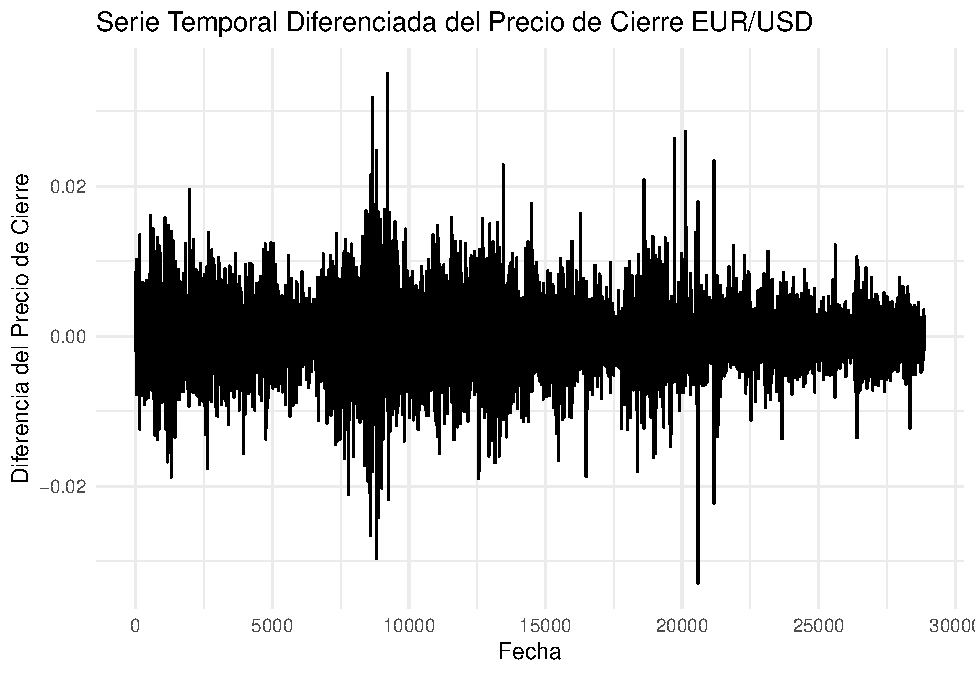
\includegraphics{bookdown_time_series_files/figure-latex/differencing-1-1.pdf}

Después de la primera diferenciación, se puede obtener que por cada tick quedó el valor del return (x-x\_ant) ue es el resultado de la aplicación de la dirferenciaciónd e primer orden. Como se aprecia, la serie ya no tiene una tendencia sino que presenta un comportamiento estacionario, sinembargo, esta serie de tiempo parece ser menos predecible que la serie de tiempo antes de la diferenciación, ya que evidentemente tiene mayor desviación estándar y por tanto un mayor Coeficiente de Variación y un menor SNR.

\section{Verificación de Estacionariedad en la Serie Diferenciada}\label{verificaciuxf3n-de-estacionariedad-en-la-serie-diferenciada}

Aplicamos nuevamente la prueba Dickey-Fuller a la serie diferenciada para verificar si ahora es estacionaria.

\begin{verbatim}
## Augmented Dickey-Fuller Test 
## alternative: stationary 
##  
## Type 1: no drift no trend 
##       lag    ADF p.value
##  [1,]   0 -169.3    0.01
##  [2,]   1 -119.0    0.01
##  [3,]   2  -99.3    0.01
##  [4,]   3  -84.8    0.01
##  [5,]   4  -75.7    0.01
##  [6,]   5  -68.7    0.01
##  [7,]   6  -64.1    0.01
##  [8,]   7  -60.1    0.01
##  [9,]   8  -56.8    0.01
## [10,]   9  -53.7    0.01
## [11,]  10  -50.9    0.01
## [12,]  11  -48.8    0.01
## [13,]  12  -47.3    0.01
## [14,]  13  -45.4    0.01
## [15,]  14  -43.7    0.01
## Type 2: with drift no trend 
##       lag    ADF p.value
##  [1,]   0 -169.3    0.01
##  [2,]   1 -119.0    0.01
##  [3,]   2  -99.3    0.01
##  [4,]   3  -84.8    0.01
##  [5,]   4  -75.7    0.01
##  [6,]   5  -68.7    0.01
##  [7,]   6  -64.1    0.01
##  [8,]   7  -60.1    0.01
##  [9,]   8  -56.8    0.01
## [10,]   9  -53.7    0.01
## [11,]  10  -50.9    0.01
## [12,]  11  -48.8    0.01
## [13,]  12  -47.3    0.01
## [14,]  13  -45.4    0.01
## [15,]  14  -43.7    0.01
## Type 3: with drift and trend 
##       lag    ADF p.value
##  [1,]   0 -169.3    0.01
##  [2,]   1 -119.0    0.01
##  [3,]   2  -99.3    0.01
##  [4,]   3  -84.9    0.01
##  [5,]   4  -75.7    0.01
##  [6,]   5  -68.7    0.01
##  [7,]   6  -64.1    0.01
##  [8,]   7  -60.1    0.01
##  [9,]   8  -56.8    0.01
## [10,]   9  -53.7    0.01
## [11,]  10  -50.9    0.01
## [12,]  11  -48.8    0.01
## [13,]  12  -47.3    0.01
## [14,]  13  -45.4    0.01
## [15,]  14  -43.7    0.01
## ---- 
## Note: in fact, p.value = 0.01 means p.value <= 0.01
\end{verbatim}

\begin{verbatim}
## $type1
##       lag        ADF p.value
##  [1,]   0 -169.27722    0.01
##  [2,]   1 -119.03874    0.01
##  [3,]   2  -99.30334    0.01
##  [4,]   3  -84.84969    0.01
##  [5,]   4  -75.69590    0.01
##  [6,]   5  -68.70703    0.01
##  [7,]   6  -64.07591    0.01
##  [8,]   7  -60.05652    0.01
##  [9,]   8  -56.77621    0.01
## [10,]   9  -53.68723    0.01
## [11,]  10  -50.91061    0.01
## [12,]  11  -48.81278    0.01
## [13,]  12  -47.29027    0.01
## [14,]  13  -45.38630    0.01
## [15,]  14  -43.68676    0.01
## 
## $type2
##       lag        ADF p.value
##  [1,]   0 -169.27433    0.01
##  [2,]   1 -119.03671    0.01
##  [3,]   2  -99.30166    0.01
##  [4,]   3  -84.84825    0.01
##  [5,]   4  -75.69462    0.01
##  [6,]   5  -68.70587    0.01
##  [7,]   6  -64.07484    0.01
##  [8,]   7  -60.05550    0.01
##  [9,]   8  -56.77525    0.01
## [10,]   9  -53.68632    0.01
## [11,]  10  -50.90973    0.01
## [12,]  11  -48.81194    0.01
## [13,]  12  -47.28946    0.01
## [14,]  13  -45.38553    0.01
## [15,]  14  -43.68601    0.01
## 
## $type3
##       lag        ADF p.value
##  [1,]   0 -169.27489    0.01
##  [2,]   1 -119.03832    0.01
##  [3,]   2  -99.30402    0.01
##  [4,]   3  -84.85094    0.01
##  [5,]   4  -75.69772    0.01
##  [6,]   5  -68.70929    0.01
##  [7,]   6  -64.07866    0.01
##  [8,]   7  -60.05942    0.01
##  [9,]   8  -56.77944    0.01
## [10,]   9  -53.69075    0.01
## [11,]  10  -50.91391    0.01
## [12,]  11  -48.81642    0.01
## [13,]  12  -47.29426    0.01
## [14,]  13  -45.39063    0.01
## [15,]  14  -43.69120    0.01
\end{verbatim}

\section{Justificación de la Transformación}\label{justificaciuxf3n-de-la-transformaciuxf3n}

Dado que la serie original no era estacionaria, fue necesario aplicar una diferenciación de primer orden para hacerla estacionaria. Esta transformación es importante para poder aplicar modelos de series de tiempo que asumen estacionariedad y para obtener mejores resultados en el análisis de patrones y predicciones.

\section{Análisis de Autocorrelación}\label{anuxe1lisis-de-autocorrelaciuxf3n}

Graficaremos las funciones de autocorrelación (ACF) y autocorrelación parcial (PACF) para observar la dependencia temporal en los datos diferenciados.

\begin{Shaded}
\begin{Highlighting}[]
\CommentTok{\# Graficar ACF y PACF de la serie diferenciada}
\FunctionTok{par}\NormalTok{(}\AttributeTok{mfrow =} \FunctionTok{c}\NormalTok{(}\DecValTok{1}\NormalTok{, }\DecValTok{2}\NormalTok{))}
\FunctionTok{Acf}\NormalTok{(forex\_diff, }\AttributeTok{main =} \StringTok{"ACF de la Serie Diferenciada"}\NormalTok{)}
\FunctionTok{Pacf}\NormalTok{(forex\_diff, }\AttributeTok{main =} \StringTok{"PACF de la Serie Diferenciada"}\NormalTok{)}
\end{Highlighting}
\end{Shaded}

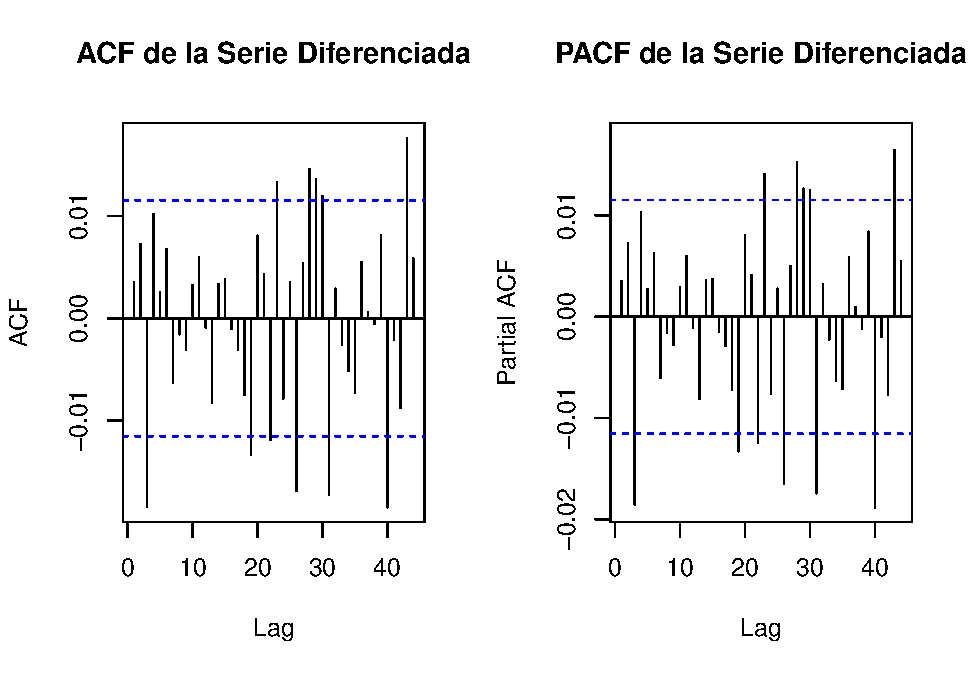
\includegraphics{bookdown_time_series_files/figure-latex/acf-pacf-1.pdf}

\begin{Shaded}
\begin{Highlighting}[]
\FunctionTok{par}\NormalTok{(}\AttributeTok{mfrow =} \FunctionTok{c}\NormalTok{(}\DecValTok{1}\NormalTok{,}\DecValTok{1}\NormalTok{))}
\end{Highlighting}
\end{Shaded}

La ACF a la izquierda muestra cómo los valores actuales de la serie diferenciada están correlacionados con sus valores en diferentes rezagos (lags). Algunos puntos de la ACF están fuera de las líneas de significancia (líneas punteadas azules), lo cual sugiere que hay correlaciones significativas en esos rezagos específicos. Este patrón puede ser indicativo de que aún existen estructuras autoregresivas o de medias móviles en la serie, incluso después de la diferenciación.

La PACF a la derecha muestra la autocorrelación de la serie diferenciada en cada rezago eliminando el efecto de los rezagos intermedios. Similar a la ACF, algunos valores están fuera de las líneas de significancia, lo que indica correlación significativa en esos rezagos específicos. Este patrón puede sugerir la presencia de efectos autoregresivos en los rezagos correspondientes.

Los picos significativos en la ACF y PACF sugieren que la serie diferenciada podría beneficiarse de un modelo ARIMA para capturar la estructura subyacente. Dependiendo de la cantidad de rezagos significativos en cada gráfico, podría ser apropiado un modelo ARIMA específico (por ejemplo, con ciertos órdenes autoregresivos y de medias móviles).

\section{Modelo ARIMA}\label{modelo-arima}

Utilizaremos \texttt{auto.arima} para identificar el mejor modelo ARIMA para los datos.

\begin{Shaded}
\begin{Highlighting}[]
\CommentTok{\# Ajuste del modelo ARIMA}
\NormalTok{forex\_arima }\OtherTok{\textless{}{-}} \FunctionTok{auto.arima}\NormalTok{(forex\_diff)}
\FunctionTok{summary}\NormalTok{(forex\_arima)}
\end{Highlighting}
\end{Shaded}

\begin{verbatim}
## Series: forex_diff 
## ARIMA(0,0,0) with zero mean 
## 
## sigma^2 = 8.978e-06:  log likelihood = 126732.8
## AIC=-253463.6   AICc=-253463.6   BIC=-253455.4
## 
## Training set error measures:
##                        ME        RMSE         MAE MPE MAPE     MASE        ACF1
## Training set 1.304966e-06 0.002996269 0.001979825 100  100 0.675058 0.003518741
\end{verbatim}

El modelo ajustado para la serie forex\_diff es un ARIMA(0,0,0) con media cero, lo que sugiere que la serie no presenta patrones autoregresivos ni de medias móviles significativos, siendo esencialmente ruido blanco. El valor de sigma\^{}2 = 8.978×10 −6 representa la varianza del error, con una alta verosimilitud (log likelihood) de 126732.8. Los criterios de información, AIC y BIC, son de -253463.6 y -253455.4, respectivamente, indicando un buen ajuste para este modelo sencillo. Las medidas de error en el conjunto de entrenamiento muestran un error medio (ME) cercano a cero (1.30e-06) y un RMSE de 0.002996, lo cual refleja una precisión razonable. La autocorrelación en el primer rezago (ACF1) es baja (0.0035), sugiriendo independencia en los residuos.

\section{Detección de Puntos de Cambio}\label{detecciuxf3n-de-puntos-de-cambio}

Usaremos la función \texttt{cpt.mean} para detectar cambios significativos en la media de la serie.

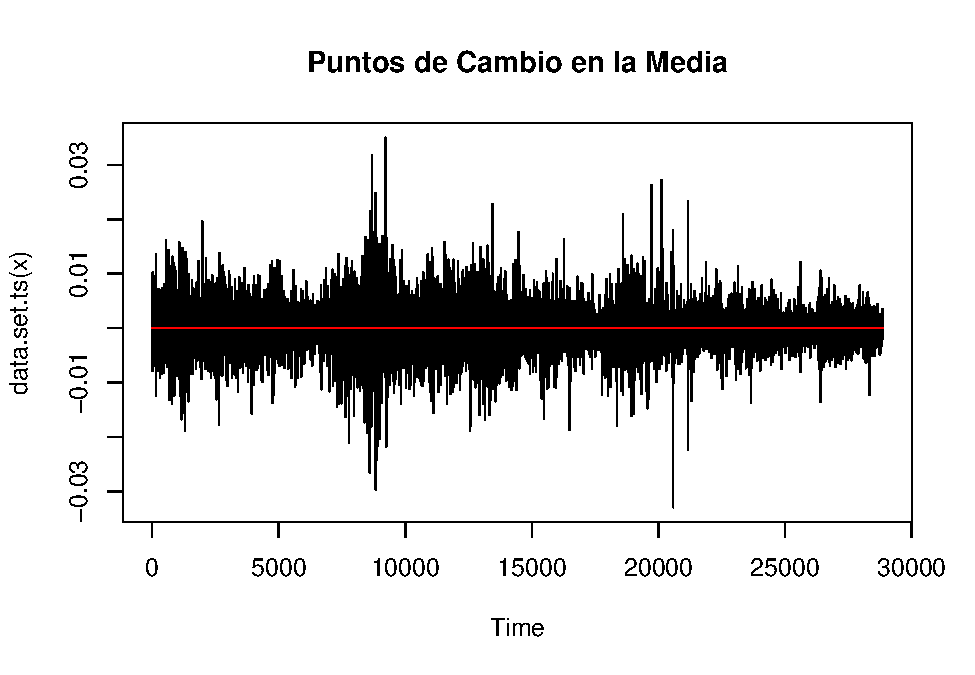
\includegraphics{bookdown_time_series_files/figure-latex/change-point-1.pdf}

No se detectaron puntos de cambio, debido a que después de la diferenciación, se convierte básicamente en ruido blanco.

\section{Media Cero de los Residuos}\label{media-cero-de-los-residuos}

Comprobamos si la media de los residuos es cero.

\begin{Shaded}
\begin{Highlighting}[]
\CommentTok{\# Prueba t en los residuos}
\NormalTok{residuals\_arima }\OtherTok{\textless{}{-}} \FunctionTok{residuals}\NormalTok{(forex\_arima)}
\NormalTok{t\_test\_residuals }\OtherTok{\textless{}{-}} \FunctionTok{t.test}\NormalTok{(residuals\_arima)}
\FunctionTok{print}\NormalTok{(t\_test\_residuals)}
\end{Highlighting}
\end{Shaded}

\begin{verbatim}
## 
##  One Sample t-test
## 
## data:  residuals_arima
## t = 0.073986, df = 28858, p-value = 0.941
## alternative hypothesis: true mean is not equal to 0
## 95 percent confidence interval:
##  -3.326619e-05  3.587612e-05
## sample estimates:
##    mean of x 
## 1.304966e-06
\end{verbatim}

La prueba t de una muestra realizada sobre los residuos (residuals\_arima) arroja un valor de 𝑡=0.073986 con 28,858 grados de libertad y un valor p de 0.941. Dado que el valor p es significativamente mayor a 0.05, no rechazamos la hipótesis nula de que la media de los residuos es igual a cero. Esto sugiere que los residuos no presentan un sesgo significativo. El intervalo de confianza del 95\% para la media de los residuos y la media estimada muy cercana a cero es consistente con un modelo bien ajustado sin tendencia sistemática en los errores.

\section{Independencia de los Residuos}\label{independencia-de-los-residuos}

Evaluamos la independencia de los residuos usando la prueba de Ljung-Box.

\begin{Shaded}
\begin{Highlighting}[]
\CommentTok{\# Prueba de independencia}
\FunctionTok{Box.test}\NormalTok{(residuals\_arima, }\AttributeTok{lag =} \DecValTok{20}\NormalTok{, }\AttributeTok{type =} \StringTok{"Ljung{-}Box"}\NormalTok{)}
\end{Highlighting}
\end{Shaded}

\begin{verbatim}
## 
##  Box-Ljung test
## 
## data:  residuals_arima
## X-squared = 30.772, df = 20, p-value = 0.05827
\end{verbatim}

Los datos cargados contienen 28,860 filas y 6 columnas de información sobre el tipo de cambio EUR/USD. La prueba de Dickey-Fuller Aumentada (ADF) realizada en tres configuraciones (sin constante ni tendencia, con constante sin tendencia, y con constante y tendencia) muestra valores ADF altamente negativos y p-valores menores o iguales a 0.01, lo que indica que la serie diferenciada es estacionaria. Además, la prueba de Box-Ljung aplicada a los residuos del modelo ARIMA arroja un valor de 30.772 con un valor p de 0.05827, lo cual sugiere que los residuos \textbf{no tienen autocorrelación significativa}, indicando independencia en los errores del modelo.

\section{Distribución de los Residuos}\label{distribuciuxf3n-de-los-residuos}

Analizaremos la normalidad de los residuos con un gráfico Q-Q.

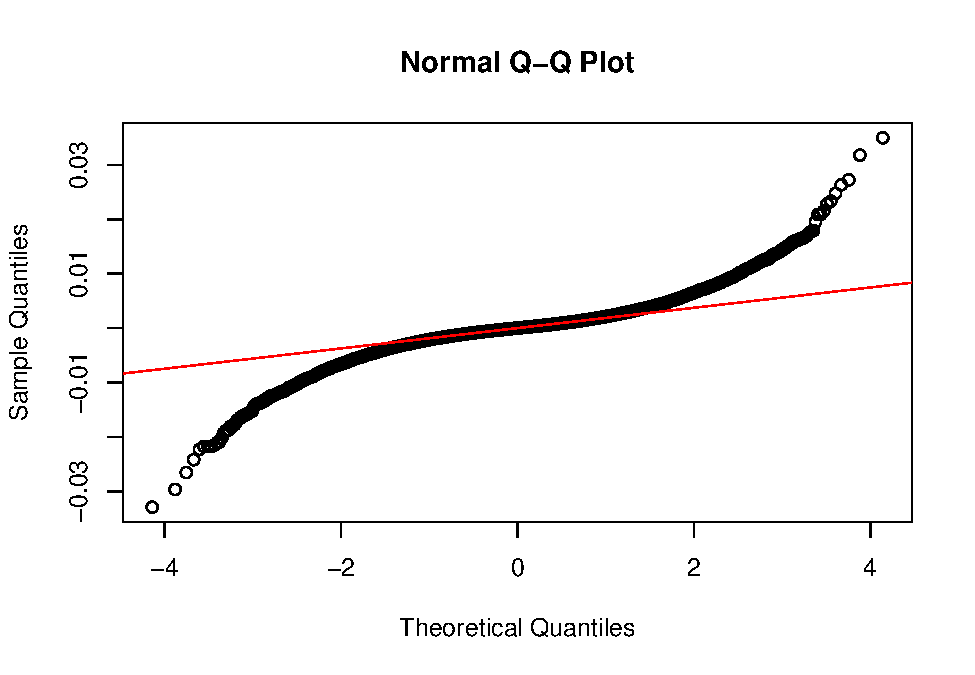
\includegraphics{bookdown_time_series_files/figure-latex/residuals-qqplot-1.pdf}

El gráfico Q-Q muestra que los residuos del modelo se alinean con la normalidad en el centro de la distribución, pero presentan desviaciones significativas en las colas. Esto sugiere que, aunque los residuos se comportan aproximadamente como una distribución normal en el centro, tienen colas más pesadas de lo esperado, lo que indica la presencia de valores extremos.

\chapter{Análisis de Series de Tiempo con el Método Holt-Winters}\label{anuxe1lisis-de-series-de-tiempo-con-el-muxe9todo-holt-winters}

Este documento realiza un análisis de series de tiempo utilizando el método de Holt-Winters aplicado exclusivamente a la columna \texttt{close} del dataset \texttt{EURUSD\_ForexTrading\_4hrs.csv}. Se utilizarán solo 6000 datos, normalizando la columna \texttt{close}, dividiendo en conjunto de entrenamiento y prueba, y calculando la métricas de error MAE en el conjunto de entrenamiento y en el conjunto de prueba.

\section{Carga de Bibliotecas y Datos}\label{carga-de-bibliotecas-y-datos}

\begin{table}
\centering
\caption{\label{tab:cargar-datos}Primeras filas del dataset EURUSD ForexTrading 4hrs Columna close}
\centering
\begin{tabular}[t]{r}
\hline
close\\
\hline
1.12274\\
\hline
1.12126\\
\hline
1.12113\\
\hline
1.12174\\
\hline
1.12712\\
\hline
1.12804\\
\hline
\end{tabular}
\end{table}

El dataset \texttt{EURUSD\_ForexTrading\_4hrs.csv} contiene datos de trading del par de divisas EUR/USD con una frecuencia de 4 horas. Solo se ha seleccionado la columna \texttt{close} con los primeros 6000 datos para este análisis.

\section{Normalización de la Columna `close'}\label{normalizaciuxf3n-de-la-columna-close}

\begin{table}
\centering
\caption{\label{tab:normalizar-close}Columna 'close' Normalizada}
\centering
\begin{tabular}[t]{r}
\hline
x\\
\hline
0.1566893\\
\hline
0.1515141\\
\hline
0.1510595\\
\hline
0.1531925\\
\hline
0.1720050\\
\hline
0.1752220\\
\hline
\end{tabular}
\end{table}

Se ha normalizado la columna \texttt{close} utilizando la técnica Min-Max, transformando los valores entre 0 y 1 para mejorar la estabilidad del modelo.

\section{Descomposición Estacional}\label{descomposiciuxf3n-estacional}

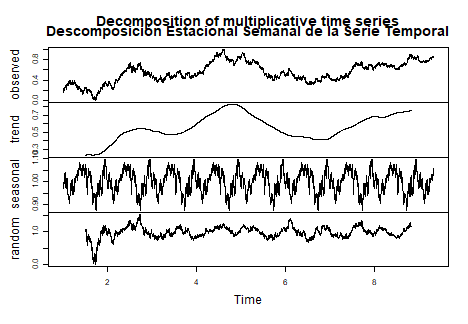
\includegraphics{bookdown_time_series_files/figure-latex/descomposicion-estacional-1.png}

Descomponemos la serie temporal en componentes de tendencia, estacionalidad y ruido para analizar los patrones internos de la serie temporal antes de aplicar el modelo.

\section{Suavizado Exponencial Simple}\label{suavizado-exponencial-simple}

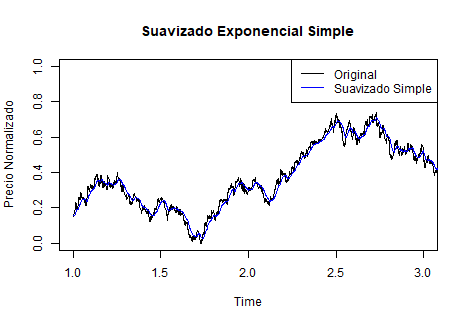
\includegraphics{bookdown_time_series_files/figure-latex/suavizado-simple-1.png}

Aplicamos el suavizado exponencial simple a la serie \texttt{close} para visualizar una versión suavizada de la serie de tiempo. Se pude observar como la señal original contiene mas ruido que la suavizada.

\section{Suavizado Exponencial Doble (Aditivo y Multiplicativo)}\label{suavizado-exponencial-doble-aditivo-y-multiplicativo}

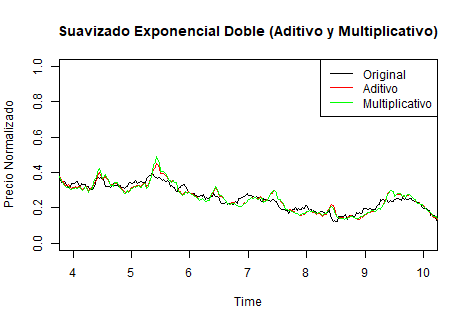
\includegraphics{bookdown_time_series_files/figure-latex/suavizado-doble-1.png}

Se puede apreciar que tanto el suavizado aditivo como el multiplicativo producen una estimación cercana a los datos originales, aunque estas señales contienen mas ruido que el suavizado simple e incluso al parecer mas que la señal original.

\section{Calculo de error}\label{calculo-de-error}

Se calcularon los errores de los modelos multiplicativo y aditivo en el dataset de training. Se usa un ajuste de 0.001 para el modelo multiplicativo, porque este requiere que todos los datos sean positivos y mayores que cero (no admite ceros), y como los datos fueron nomalizados con min-max, obligatoriamente existe al menos un valor de cero.

\begin{verbatim}
## MAE en entrenamiento (Aditivo): 0.01972768
\end{verbatim}

\begin{verbatim}
## MAE en entrenamiento (Multiplicativo): 0.05277391
\end{verbatim}

Finalmente se calcularon los errores de los modelos en el dataset de validación

\begin{verbatim}
## MAE en validación (Aditivo): 2.350168
\end{verbatim}

\begin{verbatim}
## MAE en validación (Multiplicativo): 4.704901
\end{verbatim}

Este gigantesco error es debido a que el modelo trata de predecir todo el dataset de validación de una sola vez (1238 ticks). En otros modelos predictivos en series de tiempo como redes neuronales, se usa un sliding window usando los últimos 128 ticks como entrada del modelo, se predice el siguiente, y esto se repite para cada tick, luego se promedian todos los errores y esa es la medida de desempeño de la red neuronal.

Para poder comparar el desempeño predictivo del modelo Holt-Winter con otros modelos predictivos en una serie de tiempo larga como la nuestra, probablemente se requiera usar sliding window como en las redes neuronales, se requeriría adaptar el modelo Holt-Winter para que se entrene con una ventana y prediga segmentos cortos que se concatenan y que formarían la señal pronosticada, con la cual se calcularían y promediarían los errores por tick, en lugar de tratar de predecir la serie de tiempo completa de una sola vez.

\section{Conclusiones}\label{conclusiones}

El método Holt-Winters aplicado a la columna \texttt{close} del conjunto de datos muestra que este modelo es capaz de capturar patrones de tendencia y estacionalidad en los datos de precios de cierre normalizados. Las métricas de evaluación como MAE muestran la precisión del modelo tanto en el conjunto de entrenamiento como en el conjunto de prueba, donde se puede apreciar que la predicción de todo el dataset de validación completo no es una buena forma de evaluar el desempeño de estos modelos, especialmente para comaprarlos con modelos ampliamente usados como las redes neuronales.

\chapter{Modelos Estacionarios}\label{modelos-estacionarios}

En esta sección, analizamos y predecimos series temporales usando la metodología \textbf{Box-Jenkins}. El objetivo es ajustar modelos autoregresivos integrados de media móvil (ARIMA) para encontrar patrones subyacentes en los datos y realizar predicciones futuras.

El dataset analizado contiene precios Forex EUR/USD en intervalos de 4 horas, el cual será procesado y transformado para cumplir con los requisitos de estacionariedad y ajuste de modelos ARIMA.

\section{Objetivo}\label{objetivo}

Esquematizar los modelos convencionales de series temporales mediante la metodología \textbf{Box-Jenkins} y explorar su aplicabilidad en la predicción de futuras observaciones.

\section{1. Carga y Exploración de los Datos}\label{carga-y-exploraciuxf3n-de-los-datos}

En esta sección se carga el dataset \texttt{EURUSD\_ForexTrading\_4hrs.csv}, y se realiza una exploración inicial para entender su estructura y características básicas.

\begin{verbatim}
##                  Gmt.time    open    high     low   close   volume
## 1 04.05.2003 21:00:00.000 1.12354 1.12354 1.12166 1.12274  95533.1
## 2 05.05.2003 01:00:00.000 1.12242 1.12276 1.12067 1.12126  93778.6
## 3 05.05.2003 05:00:00.000 1.12139 1.12255 1.12030 1.12113  90924.7
## 4 05.05.2003 09:00:00.000 1.12092 1.12331 1.12049 1.12174  91254.7
## 5 05.05.2003 13:00:00.000 1.12194 1.12900 1.12130 1.12712 308003.4
## 6 05.05.2003 17:00:00.000 1.12718 1.13019 1.12657 1.12804 373668.3
\end{verbatim}

\begin{verbatim}
##    Gmt.time              open            high            low       
##  Length:28860       Min.   :1.037   Min.   :1.039   Min.   :1.034  
##  Class :character   1st Qu.:1.154   1st Qu.:1.156   1st Qu.:1.152  
##  Mode  :character   Median :1.242   Median :1.244   Median :1.240  
##                     Mean   :1.254   Mean   :1.256   Mean   :1.252  
##                     3rd Qu.:1.339   3rd Qu.:1.341   3rd Qu.:1.337  
##                     Max.   :1.599   Max.   :1.604   Max.   :1.597  
##      close           volume      
##  Min.   :1.037   Min.   :     0  
##  1st Qu.:1.154   1st Qu.: 20322  
##  Median :1.242   Median : 47813  
##  Mean   :1.254   Mean   : 83079  
##  3rd Qu.:1.339   3rd Qu.:102455  
##  Max.   :1.599   Max.   :752269
\end{verbatim}

\begin{center}\rule{0.5\linewidth}{0.5pt}\end{center}

\section{2. Limpieza y Preprocesamiento de los Datos}\label{limpieza-y-preprocesamiento-de-los-datos}

Se seleccionan las columnas relevantes (en este caso, \texttt{Close}) y se convierten en una serie temporal.

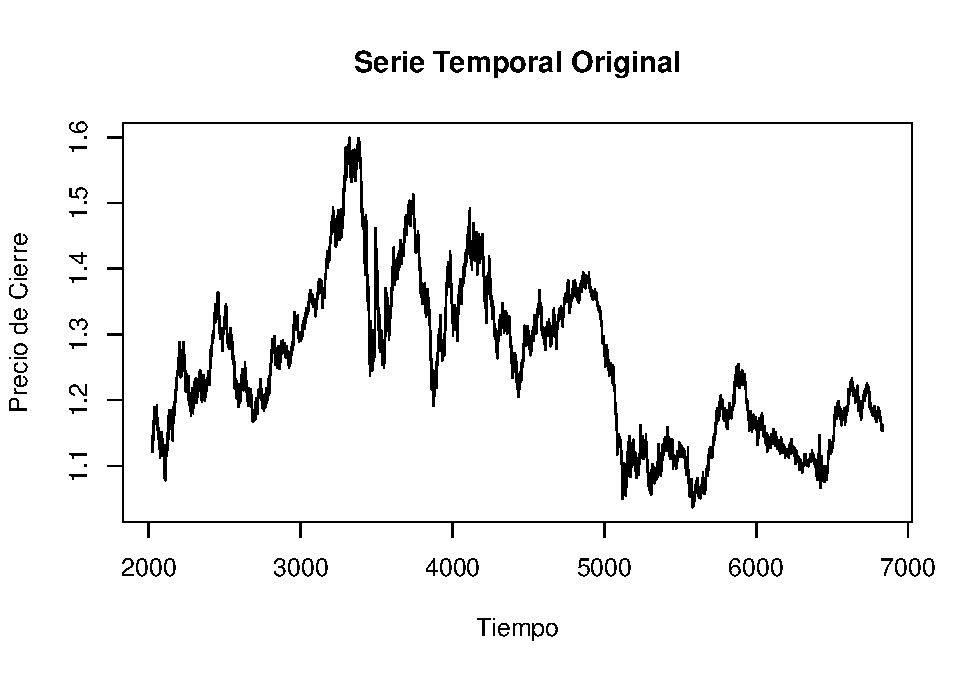
\includegraphics{bookdown_time_series_files/figure-latex/clean-data-1.pdf}

El gráfico representa la serie temporal original del precio de cierre del par Forex EUR/USD, registrado en intervalos de 4 horas. Observamos fluctuaciones significativas que reflejan los cambios en el mercado durante el período analizado. La serie muestra patrones evidentes de tendencias ascendentes y descendentes, lo que sugiere posibles componentes de largo plazo y estacionalidad que deben ser tratados en etapas posteriores del análisis, como la transformación a estacionariedad y la descomposición de los datos.

\begin{center}\rule{0.5\linewidth}{0.5pt}\end{center}

\section{3. División del Dataset en Conjuntos de Entrenamiento y Validación}\label{divisiuxf3n-del-dataset-en-conjuntos-de-entrenamiento-y-validaciuxf3n}

Se divide el dataset en 70\% para entrenamiento y 30\% para evaluación del modelo.

\section{4. Normalización de los Datos}\label{normalizaciuxf3n-de-los-datos}

La normalización es útil para estabilizar la varianza y hacer que los datos sean más adecuados para el análisis.

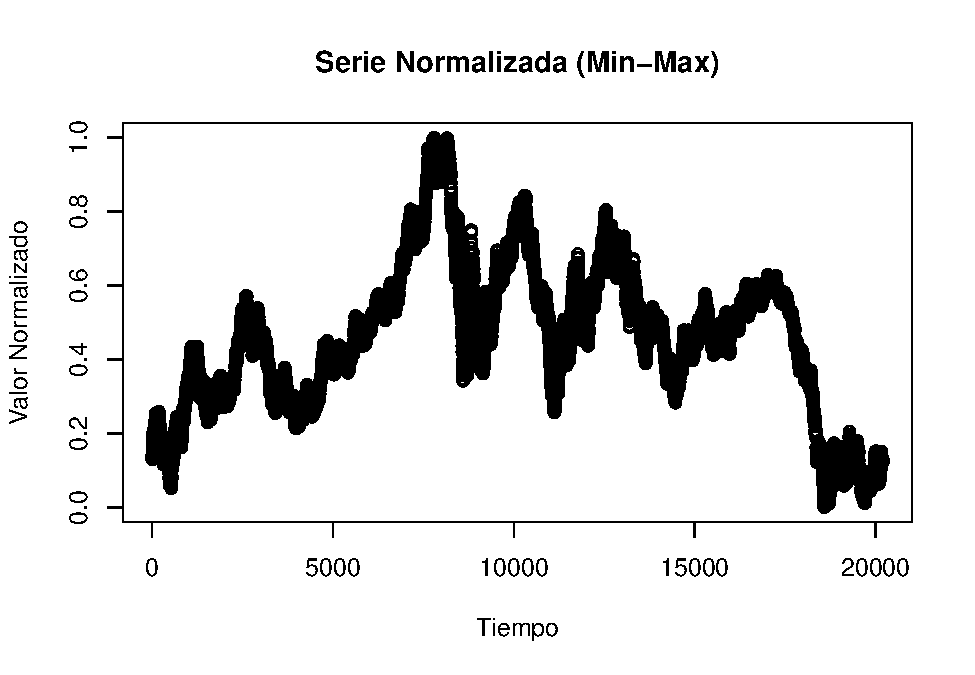
\includegraphics{bookdown_time_series_files/figure-latex/normalize-data-1.pdf}

Como se observa, el rango de los datos ahora se encuentra entre 0 y 1.

\begin{center}\rule{0.5\linewidth}{0.5pt}\end{center}

\section{5. Verificación de Estacionariedad}\label{verificaciuxf3n-de-estacionariedad}

La serie debe ser estacionaria para que los modelos ARIMA sean válidos. Evaluamos esto usando la prueba Dickey-Fuller Aumentada (ADF).

\begin{verbatim}
## Augmented Dickey-Fuller Test 
## alternative: stationary 
##  
## Type 1: no drift no trend 
##       lag    ADF p.value
##  [1,]   0 -0.861   0.372
##  [2,]   1 -0.868   0.369
##  [3,]   2 -0.874   0.367
##  [4,]   3 -0.861   0.372
##  [5,]   4 -0.874   0.367
##  [6,]   5 -0.876   0.366
##  [7,]   6 -0.878   0.365
##  [8,]   7 -0.874   0.367
##  [9,]   8 -0.875   0.367
## [10,]   9 -0.873   0.367
## [11,]  10 -0.877   0.366
## [12,]  11 -0.886   0.363
## [13,]  12 -0.885   0.363
## [14,]  13 -0.876   0.366
## Type 2: with drift no trend 
##       lag   ADF p.value
##  [1,]   0 -2.12   0.278
##  [2,]   1 -2.15   0.268
##  [3,]   2 -2.17   0.261
##  [4,]   3 -2.13   0.276
##  [5,]   4 -2.14   0.273
##  [6,]   5 -2.14   0.272
##  [7,]   6 -2.14   0.272
##  [8,]   7 -2.13   0.275
##  [9,]   8 -2.11   0.285
## [10,]   9 -2.10   0.287
## [11,]  10 -2.11   0.285
## [12,]  11 -2.09   0.292
## [13,]  12 -2.09   0.291
## [14,]  13 -2.08   0.298
## Type 3: with drift and trend 
##       lag   ADF p.value
##  [1,]   0 -2.16   0.507
##  [2,]   1 -2.19   0.496
##  [3,]   2 -2.21   0.489
##  [4,]   3 -2.17   0.505
##  [5,]   4 -2.18   0.501
##  [6,]   5 -2.18   0.501
##  [7,]   6 -2.18   0.501
##  [8,]   7 -2.17   0.504
##  [9,]   8 -2.15   0.514
## [10,]   9 -2.14   0.517
## [11,]  10 -2.15   0.514
## [12,]  11 -2.13   0.523
## [13,]  12 -2.13   0.521
## [14,]  13 -2.11   0.528
## ---- 
## Note: in fact, p.value = 0.01 means p.value <= 0.01
\end{verbatim}

\begin{verbatim}
## $type1
##       lag        ADF   p.value
##  [1,]   0 -0.8607895 0.3716268
##  [2,]   1 -0.8679287 0.3690726
##  [3,]   2 -0.8742777 0.3668010
##  [4,]   3 -0.8606220 0.3716867
##  [5,]   4 -0.8741001 0.3668646
##  [6,]   5 -0.8764373 0.3660284
##  [7,]   6 -0.8781312 0.3654224
##  [8,]   7 -0.8743629 0.3667706
##  [9,]   8 -0.8746145 0.3666806
## [10,]   9 -0.8733773 0.3671232
## [11,]  10 -0.8765659 0.3659824
## [12,]  11 -0.8856760 0.3627230
## [13,]  12 -0.8848509 0.3630182
## [14,]  13 -0.8762256 0.3661041
## 
## $type2
##       lag       ADF   p.value
##  [1,]   0 -2.124490 0.2782040
##  [2,]   1 -2.149853 0.2680589
##  [3,]   2 -2.166670 0.2613321
##  [4,]   3 -2.129695 0.2761221
##  [5,]   4 -2.138047 0.2727812
##  [6,]   5 -2.140018 0.2719927
##  [7,]   6 -2.139519 0.2721925
##  [8,]   7 -2.132869 0.2748525
##  [9,]   8 -2.108596 0.2845615
## [10,]   9 -2.102436 0.2870256
## [11,]  10 -2.108329 0.2846684
## [12,]  11 -2.089681 0.2921277
## [13,]  12 -2.093017 0.2907933
## [14,]  13 -2.075880 0.2976481
## 
## $type3
##       lag       ADF   p.value
##  [1,]   0 -2.164022 0.5068136
##  [2,]   1 -2.189210 0.4961222
##  [3,]   2 -2.205776 0.4891471
##  [4,]   3 -2.169354 0.5045398
##  [5,]   4 -2.176674 0.5014184
##  [6,]   5 -2.178475 0.5006505
##  [7,]   6 -2.177817 0.5009308
##  [8,]   7 -2.171376 0.5036774
##  [9,]   8 -2.146670 0.5142130
## [10,]   9 -2.140507 0.5168410
## [11,]  10 -2.146217 0.5144060
## [12,]  11 -2.126486 0.5228201
## [13,]  12 -2.129930 0.5213512
## [14,]  13 -2.113231 0.5284725
\end{verbatim}

El resultado de la prueba Dickey-Fuller Aumentada (ADF) muestra un estadístico Dickey-Fuller de -2.0393 con un p-valor de 0.5618, lo que indica que no podemos rechazar la hipótesis nula de que la serie tiene una raíz unitaria. Esto significa que la serie norm\_train\_data no es estacionaria. Dado que la estacionariedad es un requisito fundamental para ajustar modelos ARIMA, será necesario transformar la serie, aplicando una diferenciación para estabilizar su media y eliminar tendencias.

\begin{center}\rule{0.5\linewidth}{0.5pt}\end{center}

\section{6. Transformación a Estacionariedad}\label{transformaciuxf3n-a-estacionariedad}

Si la serie no es estacionaria, aplicamos una diferenciación para eliminar tendencias no deseadas.

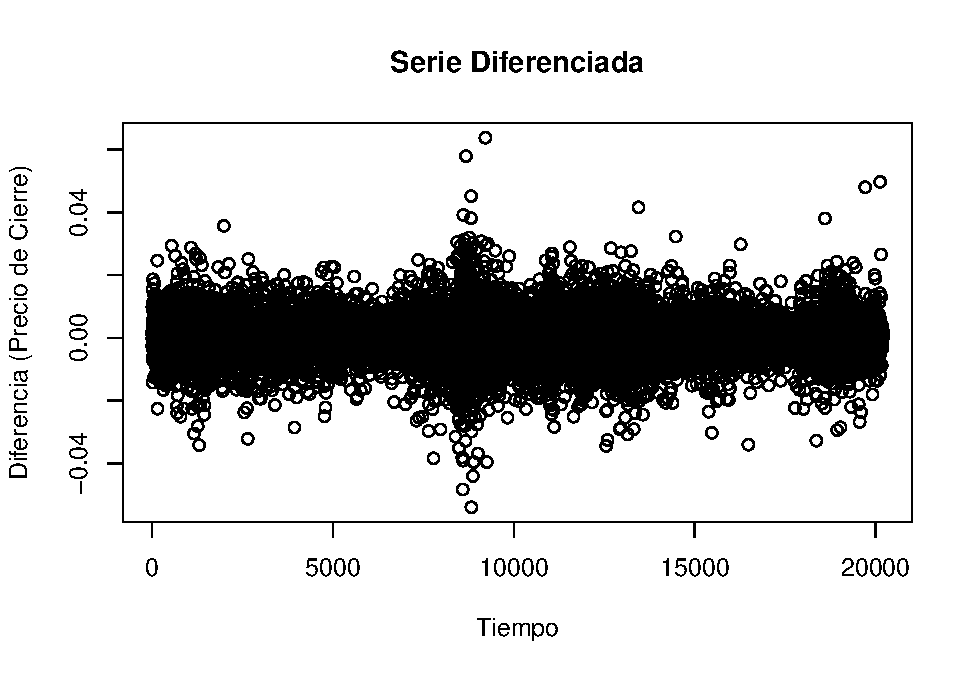
\includegraphics{bookdown_time_series_files/figure-latex/differencing-2-1.pdf}

El gráfico muestra la serie diferenciada con valores oscilando alrededor de 0, entre aproximadamente -0.02 y 0.02. Esto indica que la diferenciación logró estabilizar la media y eliminar tendencias, dejando la serie preparada para verificar su estacionariedad y ajustar un modelo ARIMA.

\begin{center}\rule{0.5\linewidth}{0.5pt}\end{center}

\section{7. Análisis ACF y PACF}\label{anuxe1lisis-acf-y-pacf}

Los gráficos de ACF y PACF ayudan a determinar los valores \(p\) y \(q\) del modelo ARIMA.

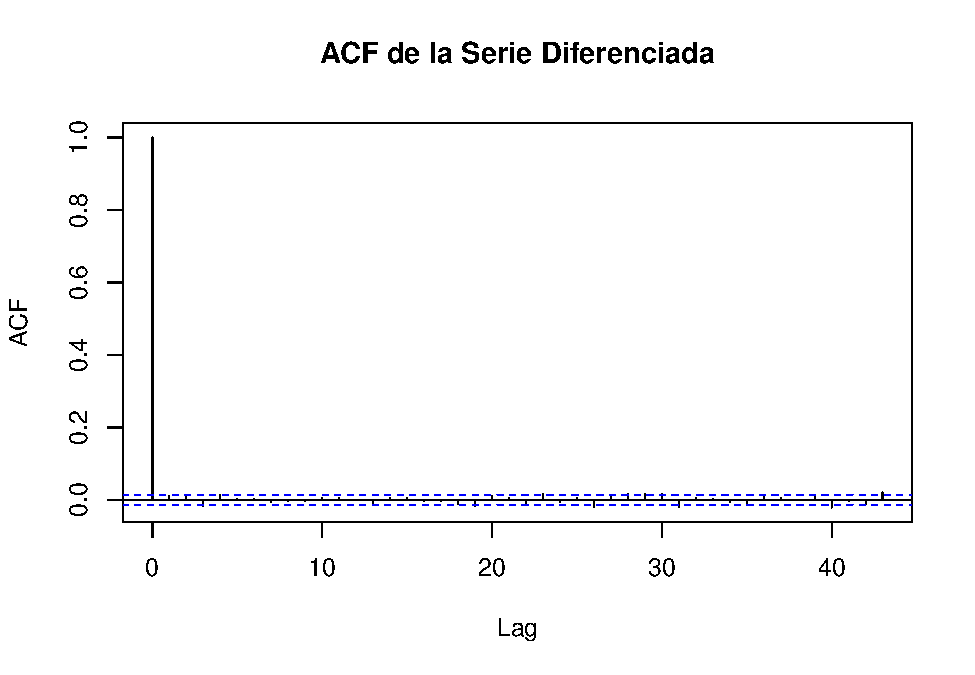
\includegraphics{bookdown_time_series_files/figure-latex/identify-parameters-1.pdf}

El gráfico de la ACF (Función de Autocorrelación) muestra un primer retardo significativo, con un valor cercano a 1.0, mientras que los retardos restantes están dentro de los intervalos de confianza (±0.05), indicando que no hay correlación significativa más allá del primer lag.

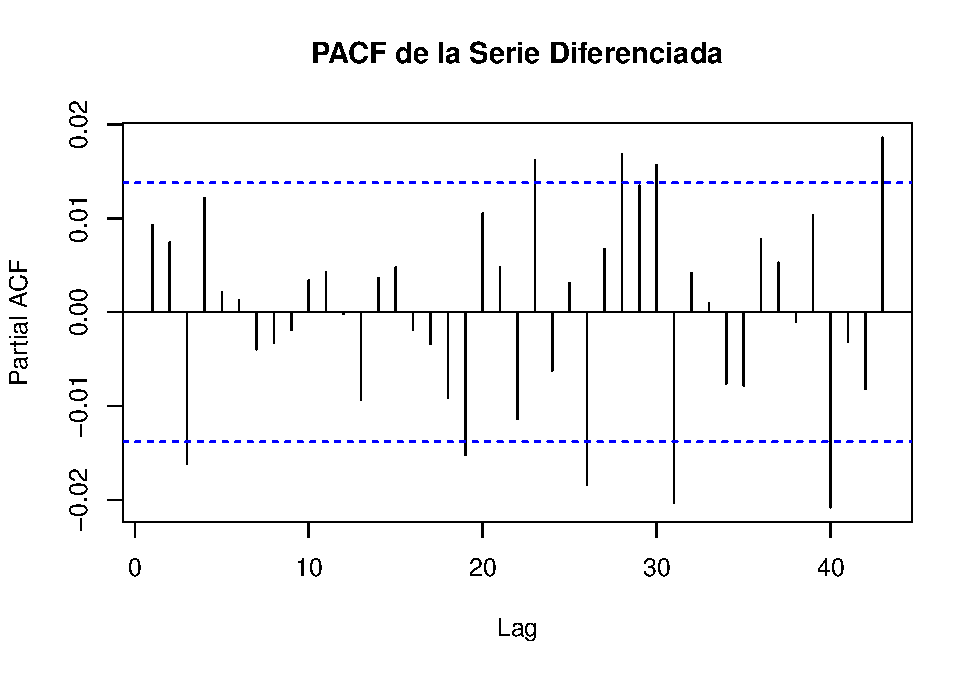
\includegraphics{bookdown_time_series_files/figure-latex/identify-parameters-2-1.pdf}

En el gráfico de la PACF (Función de Autocorrelación Parcial), los primeros retardos presentan valores significativos positivos y negativos, especialmente en los primeros lags, como el 1, 3 y 5. Esto sugiere la posible inclusión de términos autorregresivos (AR) en el modelo ARIMA.

Estos resultados guían la selección de los parámetros para ajustar un modelo ARIMA adecuado.

\begin{center}\rule{0.5\linewidth}{0.5pt}\end{center}

\section{8. Ajuste del Modelo ARIMA}\label{ajuste-del-modelo-arima}

Ajustamos un modelo ARIMA utilizando los valores \(p\), \(d\) y \(q\) obtenidos previamente. Usamos \texttt{auto.arima} para seleccionar automáticamente los mejores parámetros.

\begin{verbatim}
## Series: norm_train_data 
## ARIMA(4,1,0) 
## 
## Coefficients:
##          ar1     ar2      ar3     ar4
##       0.0095  0.0075  -0.0163  0.0121
## s.e.  0.0070  0.0070   0.0070  0.0070
## 
## sigma^2 = 3.647e-05:  log likelihood = 74553.92
## AIC=-149097.8   AICc=-149097.8   BIC=-149058.3
## 
## Training set error measures:
##                         ME        RMSE         MAE  MPE MAPE     MASE
## Training set -2.667179e-07 0.006038687 0.004067731 -Inf  Inf 1.000317
##                       ACF1
## Training set -2.599614e-05
\end{verbatim}

El modelo ajustado sobre la serie normalizada (\textbf{norm\_train\_data}) es un \textbf{ARIMA(4,1,0)} con los siguientes coeficientes: - \textbf{AR1}: 0.0095 (s.e.: 0.0070), - \textbf{AR2}: 0.0075 (s.e.: 0.0070), - \textbf{AR3}: -0.0163 (s.e.: 0.0070), - \textbf{AR4}: 0.0121 (s.e.: 0.0070).

Indicadores del modelo: - \textbf{Log-Likelihood}: 74553.92, - \textbf{AIC}: -149097.8, - \textbf{BIC}: -149058.3.

Métricas del conjunto de entrenamiento: - \textbf{RMSE}: 0.0060, - \textbf{MAE}: 0.0041, - \textbf{ACF1}: -0.000026.

Estos resultados indican un ajuste razonable del modelo a los datos normalizados, con residuos independientes y métricas de error bajas en el conjunto de entrenamiento. Sin embargo, la presencia de valores extremos en las métricas como MAPE y MPE (\(-\infty, \infty\)) sugiere posibles problemas en los cálculos debido a la normalización o a valores cercanos a cero.

\begin{center}\rule{0.5\linewidth}{0.5pt}\end{center}

\section{9. Validación del Modelo}\label{validaciuxf3n-del-modelo}

Se validan los supuestos del modelo mediante el análisis de los residuos.

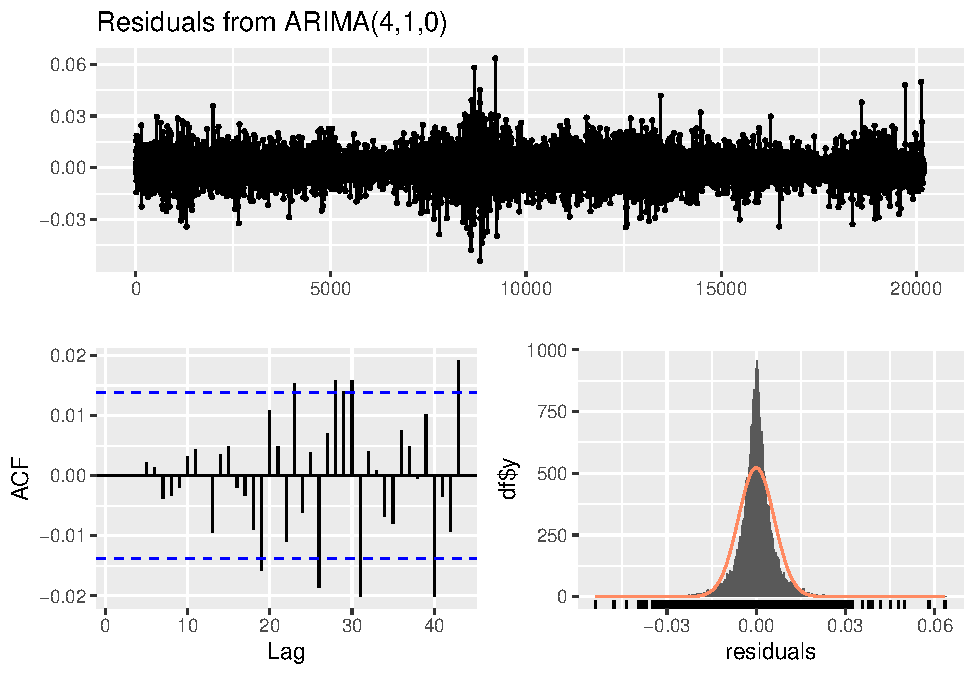
\includegraphics{bookdown_time_series_files/figure-latex/validate-model-1-1.pdf}

\begin{verbatim}
## 
##  Ljung-Box test
## 
## data:  Residuals from ARIMA(4,1,0)
## Q* = 0.91976, df = 6, p-value = 0.9885
## 
## Model df: 4.   Total lags used: 10
\end{verbatim}

El análisis de los residuos del modelo \textbf{ARIMA(4,1,0)} muestra lo siguiente:

\begin{enumerate}
\def\labelenumi{\arabic{enumi}.}
\item
  \textbf{Gráfico de Residuos}: Los residuos oscilan alrededor de 0, con valores en el rango de aproximadamente -0.02 a 0.02, sin patrones visibles ni tendencias evidentes, lo que sugiere independencia de los residuos.
\item
  \textbf{ACF de Residuos}: Los valores de autocorrelación de los residuos están mayoritariamente dentro de los intervalos de confianza (±0.02), excepto por algunos picos en retardos altos, indicando que los residuos son casi ruido blanco.
\item
  \textbf{Distribución de Residuos}: El histograma muestra una distribución aproximadamente normal centrada en 0, corroborada por la curva de densidad ajustada, lo que valida la suposición de normalidad en los residuos.
\end{enumerate}

Estos resultados indican que el modelo ajustado cumple los supuestos de independencia y normalidad de los residuos, validando su uso para predicción.

\begin{verbatim}
## 
##  Box-Ljung test
## 
## data:  model$residuals
## X-squared = 0.91976, df = 10, p-value = 0.9999
\end{verbatim}

El resultado de la prueba \textbf{Box-Ljung} para los residuos del modelo muestra un estadístico \(X^2 = 0.91976\) con \(df = 10\) grados de libertad y un \(p\text{-valor} = 0.9999\). Dado que el \(p\text{-valor} \gg 0.05\), no se puede rechazar la hipótesis nula de que los residuos son ruido blanco, confirmando la independencia de los residuos y validando el ajuste del modelo.

Dado que el \(p\text{-valor} > 0.05\), no se puede rechazar la hipótesis nula de que los residuos son ruido blanco. Esto confirma que los residuos del modelo no presentan autocorrelación significativa, validando así el ajuste del modelo ARIMA.

\begin{center}\rule{0.5\linewidth}{0.5pt}\end{center}

\section{10. Predicción}\label{predicciuxf3n}

Realizamos predicciones para los próximos intervalos usando el modelo ajustado.

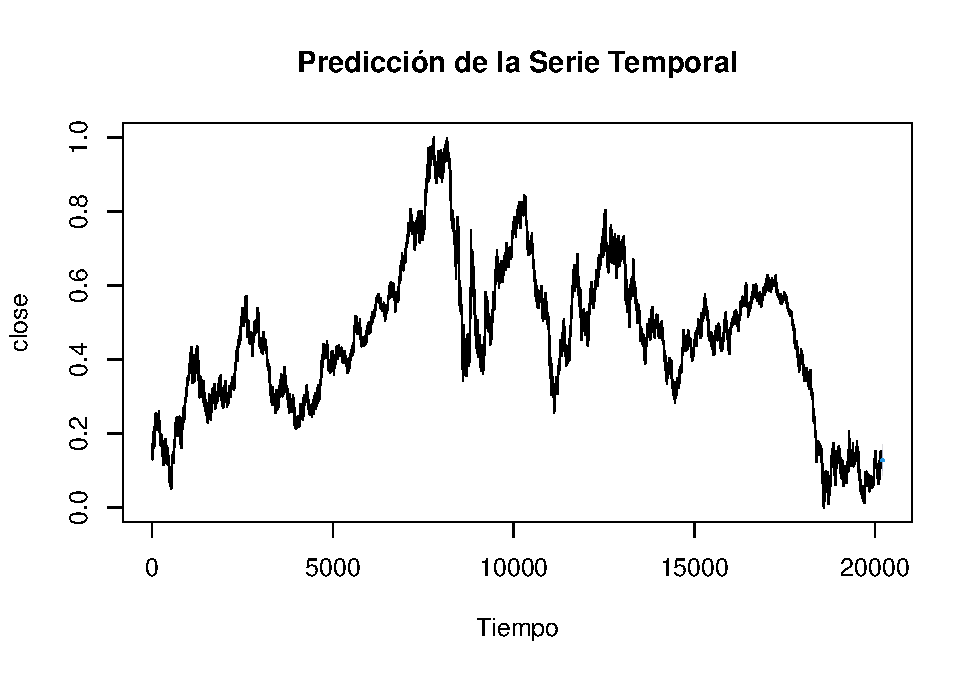
\includegraphics{bookdown_time_series_files/figure-latex/forecast-1.pdf}

El gráfico muestra la serie temporal original superpuesta con la predicción generada por el modelo \textbf{ARIMA(4,1,0)}. Aunque las predicciones siguen la tendencia general de la serie, el resultado es muy similar al original debido a que el modelo representa una diferenciación de primer orden, capturando únicamente cambios incrementales sin agregar términos de media móvil (\(q\)) y usando 4 para el autorregresivo.

\begin{center}\rule{0.5\linewidth}{0.5pt}\end{center}

\section{11. Evaluación de Predicciones}\label{evaluaciuxf3n-de-predicciones}

Se evalúan las predicciones contra los datos de prueba usando métricas de error.

\begin{verbatim}
## MAE en el conjunto de entrenamiento: 0.004067731
\end{verbatim}

\begin{verbatim}
## MAE en el conjunto de prueba: 0.07728354
\end{verbatim}

El error absoluto medio (MAE) del modelo en el conjunto de entrenamiento es \textbf{0.00406}, mientras que en el conjunto de prueba es significativamente mayor, con un valor de \textbf{0.0772}. Esto sugiere que el modelo se ajusta bien a los datos de entrenamiento, pero tiene dificultades para generalizar a datos no vistos, indicando un posible sobreajuste o la necesidad de mejorar la capacidad predictiva del modelo.

\begin{center}\rule{0.5\linewidth}{0.5pt}\end{center}

\section{12. Conclusiones}\label{conclusiones-1}

Las siguientes son las conlusiones de las actividares realizadas:

\begin{itemize}
\tightlist
\item
  \textbf{Ajuste del Modelo ARIMA}:

  \begin{itemize}
  \tightlist
  \item
    Un modelo \textbf{ARIMA(4,1,0)}, incorporó términos autorregresivos (\(p = 4\)) y mostró mejoras sutiles respecto al ARIMA(0,1,0) probado inicialmente en los indicadores como \textbf{log-likelihood = 74553.92} y \textbf{AIC = -149097.8}, con residuos que cumplen las suposiciones de ruido blanco y normalidad.
  \end{itemize}
\item
  \textbf{Validación del Modelo}:

  \begin{itemize}
  \tightlist
  \item
    La prueba \textbf{Box-Ljung} confirmó que los residuos del modelo \textbf{ARIMA(4,1,0)} son independientes y no presentan autocorrelación significativa (\(p\text{-valor} = 0.9999\)).
  \item
    Los residuos mostraron una distribución aproximadamente normal, validando aún más la calidad del modelo ajustado.
  \end{itemize}
\item
  \textbf{Evaluación de Predicciones}:

  \begin{itemize}
  \tightlist
  \item
    El \textbf{MAE en el conjunto de entrenamiento} fue de \textbf{0.00406}, mientras que en el conjunto de prueba aumentó significativamente a \textbf{0.07728354}, lo que indica que el modelo tiene dificultades para generalizar a datos no vistos, posiblemente debido a sobreajuste o características complejas no capturadas.
  \end{itemize}
\item
  \textbf{Limitaciones y Mejoras}:

  \begin{itemize}
  \tightlist
  \item
    Aunque el modelo \textbf{ARIMA(4,1,0)} ofrece un mejor ajuste que el \textbf{ARIMA(0,1,0)}, no logra reducir el error en el conjunto de prueba de forma significativa.
  \item
    Sería recomendable explorar modelos más avanzados, como \textbf{SARIMA}, para capturar componentes estacionales, o incluir variables exógenas para mejorar las predicciones.
  \end{itemize}
\end{itemize}

El uso de la metodología \textbf{Box-Jenkins} permitió identificar patrones y ajustar modelos que explican las características principales de la serie temporal. Sin embargo, la discrepancia entre el desempeño en los conjuntos de entrenamiento y prueba resalta la necesidad de modelos más robustos para mejorar la capacidad predictiva.

\chapter{Modelos Estacionarios en series de tiempo}\label{modelos-estacionarios-en-series-de-tiempo}

El Algoritmo prophet permite pronosticar series de tiempo adaptandose a tendencias no lineales, con estacionalidad e involucrando dias festivos o periodos de vacaciones.

Realizaremos la prediccion de nuestros serie basados en el Modelo Prophet.

\section{1. Carga y Preprocesamiento del Dataset}\label{carga-y-preprocesamiento-del-dataset}

Cargamos los paquetes necesarios y el dataset EURUSD\_ForexTrading\_4hrs.csv que contiene los tipos de cambio Euro Dolar históricos de 2003 a 2021

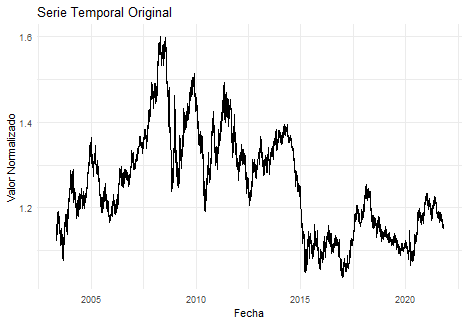
\includegraphics{bookdown_time_series_files/figure-latex/unnamed-chunk-12-1.png}

\section{2. Análisis de Estacionalidad}\label{anuxe1lisis-de-estacionalidad-1}

Realizamos el analisis de estacionariedad para realizar la técnica de modelado ARIMA, donde se asumen que la serie temporal es estacionaria. Si no lo es, las predicciones pueden ser inexactas. Para analizar la estacionariedad de la serie temporal, se utilizó la descomposición STL, la función de autocorrelación (ACF) y la prueba de Augmented Dickey-Fuller (ADF). Los pasos y los resultados fueron los siguientes:

\begin{enumerate}
\def\labelenumi{\arabic{enumi}.}
\item
  \textbf{Descomposición de la Serie Temporal}:

  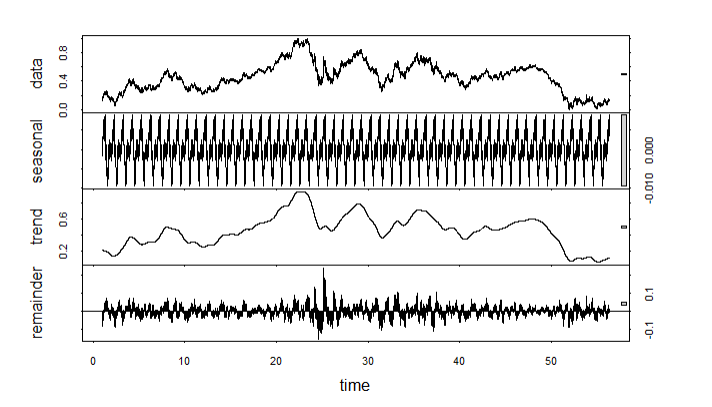
\includegraphics{images/clipboard-2193911821.png}

  \begin{itemize}
  \item
    Se descompuso la serie en sus componentes: tendencia, estacionalidad y residuo.
  \item
    El gráfico resultante muestra que la serie presenta una componente estacional marcada (gráfico en la parte superior).
  \end{itemize}
\item
  \textbf{Función de Autocorrelación (ACF)}:\\
  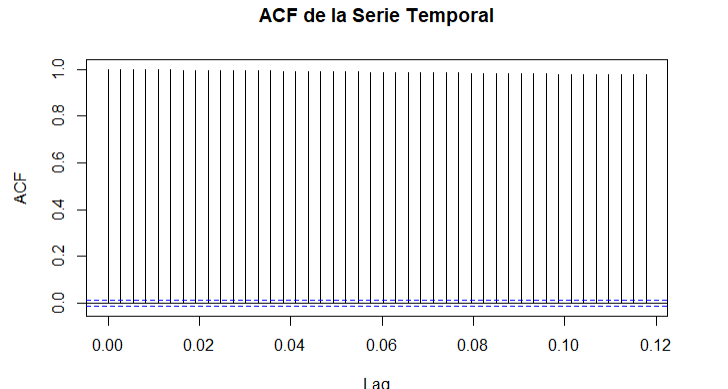
\includegraphics{images/clipboard-928318317.png}

  \begin{itemize}
  \tightlist
  \item
    El gráfico de la ACF mostró correlaciones significativas en muchos rezagos, indicando que la serie no es estacionaria.
  \end{itemize}
\item
  \textbf{Prueba ADF (Augmented Dickey-Fuller)}:

  \begin{itemize}
  \tightlist
  \item
    El valor p obtenido en el test ADF fue \texttt{0.5523948}. Como este valor es mayor a 0.05, no se puede rechazar la hipótesis nula de que la serie tiene una raíz unitaria. Por lo tanto, \textbf{la serie no es estacionaria}.
  \end{itemize}
\end{enumerate}

Como se observa, después de la diferenciación la serie se vuelve estacionaria, esto se usará solo en ARIMA que requiere que la serie de tiempo sea estacionaria, para prophet y ets en cambio, la predicción se beneficia de la estacionalidad únicamente, mas no requieren de estacionariedad.

\section{3. Ajuste y Predicciones con Prophet}\label{ajuste-y-predicciones-con-prophet}

Las predicciones con Prophet tiene muchas ventajas,permite trabajar con series temporales incorporando periodos con estacionalidad, tendencia y datos irregulares con un modelo robusto, la estructuracion y ajuste del modelo son sencillas y sirven como inside para comparacion con otros modelos.

Procedemos con los ajustes necesarios para la prediccion con prophet:

\begin{verbatim}
## Datos de entrenamiento filtrados al último año: 1558 registros
\end{verbatim}

\begin{verbatim}
## Puntos de cambio detectados: 131
\end{verbatim}

\begin{verbatim}
## Prophet MAE (Training - Último Año): 0.009706115
\end{verbatim}

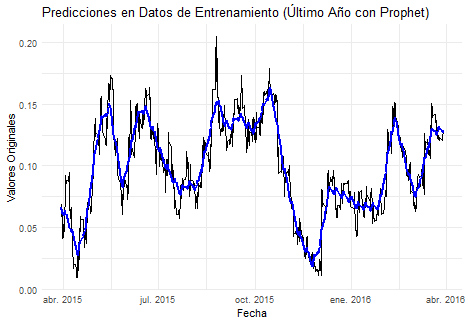
\includegraphics{bookdown_time_series_files/figure-latex/unnamed-chunk-13-1.png}

\section{4. Ajuste y Predicción en Validación}\label{ajuste-y-predicciuxf3n-en-validaciuxf3n}

El proceso de validacion se realizo entrenado el modelo con la tecnica sliding window con stride 6 que corresponde a un dia para predecir los siguentes, se utilizo para encontrar subcobjutos que cumplan con condiciones especificas. Para realizar esta seleccion se valido la tecnica Rolling window que es un sliding window son stride 1, es decir que va tick a tick, mientras en sliding window presento mejor ajuste a nuestro data set saltando un numero de ticks diario.

\begin{verbatim}
## Día 1/365 - MAE Segmento: 0.0140 - MAE Acumulado: 0.0140Día 2/365 - MAE Segmento: 0.0109 - MAE Acumulado: 0.0124Día 3/365 - MAE Segmento: 0.0115 - MAE Acumulado: 0.0121Día 4/365 - MAE Segmento: 0.0091 - MAE Acumulado: 0.0114Día 5/365 - MAE Segmento: 0.0107 - MAE Acumulado: 0.0112Día 6/365 - MAE Segmento: 0.0174 - MAE Acumulado: 0.0123Día 7/365 - MAE Segmento: 0.0052 - MAE Acumulado: 0.0113Día 8/365 - MAE Segmento: 0.0073 - MAE Acumulado: 0.0108Día 9/365 - MAE Segmento: 0.0092 - MAE Acumulado: 0.0106Día 10/365 - MAE Segmento: 0.0107 - MAE Acumulado: 0.0106Día 11/365 - MAE Segmento: 0.0110 - MAE Acumulado: 0.0106Día 12/365 - MAE Segmento: 0.0074 - MAE Acumulado: 0.0104Día 13/365 - MAE Segmento: 0.0082 - MAE Acumulado: 0.0102Día 14/365 - MAE Segmento: 0.0109 - MAE Acumulado: 0.0102Día 15/365 - MAE Segmento: 0.0065 - MAE Acumulado: 0.0100Día 16/365 - MAE Segmento: 0.0118 - MAE Acumulado: 0.0101Día 17/365 - MAE Segmento: 0.0174 - MAE Acumulado: 0.0105Día 18/365 - MAE Segmento: 0.0246 - MAE Acumulado: 0.0113Día 19/365 - MAE Segmento: 0.0171 - MAE Acumulado: 0.0116Día 20/365 - MAE Segmento: 0.0192 - MAE Acumulado: 0.0120Día 21/365 - MAE Segmento: 0.0137 - MAE Acumulado: 0.0121Día 22/365 - MAE Segmento: 0.0180 - MAE Acumulado: 0.0123Día 23/365 - MAE Segmento: 0.0270 - MAE Acumulado: 0.0130Día 24/365 - MAE Segmento: 0.0210 - MAE Acumulado: 0.0133Día 25/365 - MAE Segmento: 0.0386 - MAE Acumulado: 0.0143Día 26/365 - MAE Segmento: 0.0522 - MAE Acumulado: 0.0158Día 27/365 - MAE Segmento: 0.0617 - MAE Acumulado: 0.0175Día 28/365 - MAE Segmento: 0.0562 - MAE Acumulado: 0.0189Día 29/365 - MAE Segmento: 0.0498 - MAE Acumulado: 0.0199Día 30/365 - MAE Segmento: 0.0610 - MAE Acumulado: 0.0213Día 31/365 - MAE Segmento: 0.0611 - MAE Acumulado: 0.0226Día 32/365 - MAE Segmento: 0.0560 - MAE Acumulado: 0.0236Día 33/365 - MAE Segmento: 0.0592 - MAE Acumulado: 0.0247Día 34/365 - MAE Segmento: 0.0614 - MAE Acumulado: 0.0258Día 35/365 - MAE Segmento: 0.0560 - MAE Acumulado: 0.0266Día 36/365 - MAE Segmento: 0.0447 - MAE Acumulado: 0.0271Día 37/365 - MAE Segmento: 0.0344 - MAE Acumulado: 0.0273Día 38/365 - MAE Segmento: 0.0317 - MAE Acumulado: 0.0275Día 39/365 - MAE Segmento: 0.0342 - MAE Acumulado: 0.0276Día 40/365 - MAE Segmento: 0.0401 - MAE Acumulado: 0.0279Día 41/365 - MAE Segmento: 0.0456 - MAE Acumulado: 0.0284Día 42/365 - MAE Segmento: 0.0407 - MAE Acumulado: 0.0287Día 43/365 - MAE Segmento: 0.0297 - MAE Acumulado: 0.0287Día 44/365 - MAE Segmento: 0.0356 - MAE Acumulado: 0.0288Día 45/365 - MAE Segmento: 0.0425 - MAE Acumulado: 0.0292Día 46/365 - MAE Segmento: 0.0386 - MAE Acumulado: 0.0294Día 47/365 - MAE Segmento: 0.0313 - MAE Acumulado: 0.0294Día 48/365 - MAE Segmento: 0.0389 - MAE Acumulado: 0.0296Día 49/365 - MAE Segmento: 0.0583 - MAE Acumulado: 0.0302Día 50/365 - MAE Segmento: 0.0517 - MAE Acumulado: 0.0306Día 51/365 - MAE Segmento: 0.0477 - MAE Acumulado: 0.0309Día 52/365 - MAE Segmento: 0.0471 - MAE Acumulado: 0.0313Día 53/365 - MAE Segmento: 0.0372 - MAE Acumulado: 0.0314Día 54/365 - MAE Segmento: 0.0393 - MAE Acumulado: 0.0315Día 55/365 - MAE Segmento: 0.0407 - MAE Acumulado: 0.0317Día 56/365 - MAE Segmento: 0.0425 - MAE Acumulado: 0.0319Día 57/365 - MAE Segmento: 0.0375 - MAE Acumulado: 0.0320Día 58/365 - MAE Segmento: 0.0278 - MAE Acumulado: 0.0319Día 59/365 - MAE Segmento: 0.0192 - MAE Acumulado: 0.0317Día 60/365 - MAE Segmento: 0.0156 - MAE Acumulado: 0.0314Día 61/365 - MAE Segmento: 0.0076 - MAE Acumulado: 0.0310Día 62/365 - MAE Segmento: 0.0128 - MAE Acumulado: 0.0307Día 63/365 - MAE Segmento: 0.0090 - MAE Acumulado: 0.0304Día 64/365 - MAE Segmento: 0.0115 - MAE Acumulado: 0.0301Día 65/365 - MAE Segmento: 0.0065 - MAE Acumulado: 0.0297Día 66/365 - MAE Segmento: 0.0037 - MAE Acumulado: 0.0293Día 67/365 - MAE Segmento: 0.0123 - MAE Acumulado: 0.0291Día 68/365 - MAE Segmento: 0.0250 - MAE Acumulado: 0.0290Día 69/365 - MAE Segmento: 0.0343 - MAE Acumulado: 0.0291Día 70/365 - MAE Segmento: 0.0385 - MAE Acumulado: 0.0292Día 71/365 - MAE Segmento: 0.0284 - MAE Acumulado: 0.0292Día 72/365 - MAE Segmento: 0.0239 - MAE Acumulado: 0.0291Día 73/365 - MAE Segmento: 0.0285 - MAE Acumulado: 0.0291Día 74/365 - MAE Segmento: 0.0308 - MAE Acumulado: 0.0292Día 75/365 - MAE Segmento: 0.0247 - MAE Acumulado: 0.0291Día 76/365 - MAE Segmento: 0.0189 - MAE Acumulado: 0.0290Día 77/365 - MAE Segmento: 0.0145 - MAE Acumulado: 0.0288Día 78/365 - MAE Segmento: 0.0100 - MAE Acumulado: 0.0285Día 79/365 - MAE Segmento: 0.0058 - MAE Acumulado: 0.0283Día 80/365 - MAE Segmento: 0.0105 - MAE Acumulado: 0.0280Día 81/365 - MAE Segmento: 0.0051 - MAE Acumulado: 0.0277Día 82/365 - MAE Segmento: 0.0110 - MAE Acumulado: 0.0275Día 83/365 - MAE Segmento: 0.0142 - MAE Acumulado: 0.0274Día 84/365 - MAE Segmento: 0.0085 - MAE Acumulado: 0.0272Día 85/365 - MAE Segmento: 0.0112 - MAE Acumulado: 0.0270Día 86/365 - MAE Segmento: 0.0175 - MAE Acumulado: 0.0269Día 87/365 - MAE Segmento: 0.0230 - MAE Acumulado: 0.0268Día 88/365 - MAE Segmento: 0.0234 - MAE Acumulado: 0.0268Día 89/365 - MAE Segmento: 0.0196 - MAE Acumulado: 0.0267Día 90/365 - MAE Segmento: 0.0218 - MAE Acumulado: 0.0266Día 91/365 - MAE Segmento: 0.0232 - MAE Acumulado: 0.0266Día 92/365 - MAE Segmento: 0.0304 - MAE Acumulado: 0.0266Día 93/365 - MAE Segmento: 0.0364 - MAE Acumulado: 0.0267Día 94/365 - MAE Segmento: 0.0489 - MAE Acumulado: 0.0270Día 95/365 - MAE Segmento: 0.0497 - MAE Acumulado: 0.0272Día 96/365 - MAE Segmento: 0.0436 - MAE Acumulado: 0.0274Día 97/365 - MAE Segmento: 0.0480 - MAE Acumulado: 0.0276Día 98/365 - MAE Segmento: 0.0355 - MAE Acumulado: 0.0277Día 99/365 - MAE Segmento: 0.0219 - MAE Acumulado: 0.0276Día 100/365 - MAE Segmento: 0.0172 - MAE Acumulado: 0.0275Día 101/365 - MAE Segmento: 0.0197 - MAE Acumulado: 0.0274Día 102/365 - MAE Segmento: 0.0360 - MAE Acumulado: 0.0275Día 103/365 - MAE Segmento: 0.0592 - MAE Acumulado: 0.0278Día 104/365 - MAE Segmento: 0.0605 - MAE Acumulado: 0.0282Día 105/365 - MAE Segmento: 0.0563 - MAE Acumulado: 0.0284Día 106/365 - MAE Segmento: 0.0466 - MAE Acumulado: 0.0286Día 107/365 - MAE Segmento: 0.0488 - MAE Acumulado: 0.0288Día 108/365 - MAE Segmento: 0.0402 - MAE Acumulado: 0.0289Día 109/365 - MAE Segmento: 0.0410 - MAE Acumulado: 0.0290Día 110/365 - MAE Segmento: 0.0491 - MAE Acumulado: 0.0292Día 111/365 - MAE Segmento: 0.0654 - MAE Acumulado: 0.0295Día 112/365 - MAE Segmento: 0.0621 - MAE Acumulado: 0.0298Día 113/365 - MAE Segmento: 0.0496 - MAE Acumulado: 0.0300Día 114/365 - MAE Segmento: 0.0427 - MAE Acumulado: 0.0301Día 115/365 - MAE Segmento: 0.0456 - MAE Acumulado: 0.0302Día 116/365 - MAE Segmento: 0.0412 - MAE Acumulado: 0.0303Día 117/365 - MAE Segmento: 0.0478 - MAE Acumulado: 0.0305Día 118/365 - MAE Segmento: 0.0354 - MAE Acumulado: 0.0305Día 119/365 - MAE Segmento: 0.0177 - MAE Acumulado: 0.0304Día 120/365 - MAE Segmento: 0.0134 - MAE Acumulado: 0.0303Día 121/365 - MAE Segmento: 0.0094 - MAE Acumulado: 0.0301Día 122/365 - MAE Segmento: 0.0122 - MAE Acumulado: 0.0299Día 123/365 - MAE Segmento: 0.0175 - MAE Acumulado: 0.0298Día 124/365 - MAE Segmento: 0.0100 - MAE Acumulado: 0.0297Día 125/365 - MAE Segmento: 0.0037 - MAE Acumulado: 0.0295Día 126/365 - MAE Segmento: 0.0149 - MAE Acumulado: 0.0294Día 127/365 - MAE Segmento: 0.0202 - MAE Acumulado: 0.0293Día 128/365 - MAE Segmento: 0.0042 - MAE Acumulado: 0.0291Día 129/365 - MAE Segmento: 0.0108 - MAE Acumulado: 0.0289Día 130/365 - MAE Segmento: 0.0207 - MAE Acumulado: 0.0289Día 131/365 - MAE Segmento: 0.0282 - MAE Acumulado: 0.0289Día 132/365 - MAE Segmento: 0.0253 - MAE Acumulado: 0.0288Día 133/365 - MAE Segmento: 0.0291 - MAE Acumulado: 0.0288Día 134/365 - MAE Segmento: 0.0284 - MAE Acumulado: 0.0288Día 135/365 - MAE Segmento: 0.0444 - MAE Acumulado: 0.0290Día 136/365 - MAE Segmento: 0.0503 - MAE Acumulado: 0.0291Día 137/365 - MAE Segmento: 0.0352 - MAE Acumulado: 0.0292Día 138/365 - MAE Segmento: 0.0280 - MAE Acumulado: 0.0292Día 139/365 - MAE Segmento: 0.0215 - MAE Acumulado: 0.0291Día 140/365 - MAE Segmento: 0.0112 - MAE Acumulado: 0.0290Día 141/365 - MAE Segmento: 0.0144 - MAE Acumulado: 0.0289Día 142/365 - MAE Segmento: 0.0320 - MAE Acumulado: 0.0289Día 143/365 - MAE Segmento: 0.0320 - MAE Acumulado: 0.0289Día 144/365 - MAE Segmento: 0.0286 - MAE Acumulado: 0.0289Día 145/365 - MAE Segmento: 0.0193 - MAE Acumulado: 0.0288Día 146/365 - MAE Segmento: 0.0236 - MAE Acumulado: 0.0288Día 147/365 - MAE Segmento: 0.0338 - MAE Acumulado: 0.0288Día 148/365 - MAE Segmento: 0.0398 - MAE Acumulado: 0.0289Día 149/365 - MAE Segmento: 0.0312 - MAE Acumulado: 0.0289Día 150/365 - MAE Segmento: 0.0426 - MAE Acumulado: 0.0290Día 151/365 - MAE Segmento: 0.0303 - MAE Acumulado: 0.0290Día 152/365 - MAE Segmento: 0.0319 - MAE Acumulado: 0.0290Día 153/365 - MAE Segmento: 0.0242 - MAE Acumulado: 0.0290Día 154/365 - MAE Segmento: 0.0142 - MAE Acumulado: 0.0289Día 155/365 - MAE Segmento: 0.0203 - MAE Acumulado: 0.0289Día 156/365 - MAE Segmento: 0.0354 - MAE Acumulado: 0.0289Día 157/365 - MAE Segmento: 0.0376 - MAE Acumulado: 0.0290Día 158/365 - MAE Segmento: 0.0349 - MAE Acumulado: 0.0290Día 159/365 - MAE Segmento: 0.0386 - MAE Acumulado: 0.0291Día 160/365 - MAE Segmento: 0.0414 - MAE Acumulado: 0.0291Día 161/365 - MAE Segmento: 0.0411 - MAE Acumulado: 0.0292Día 162/365 - MAE Segmento: 0.0460 - MAE Acumulado: 0.0293Día 163/365 - MAE Segmento: 0.0366 - MAE Acumulado: 0.0294Día 164/365 - MAE Segmento: 0.0274 - MAE Acumulado: 0.0293Día 165/365 - MAE Segmento: 0.0193 - MAE Acumulado: 0.0293Día 166/365 - MAE Segmento: 0.0193 - MAE Acumulado: 0.0292Día 167/365 - MAE Segmento: 0.0234 - MAE Acumulado: 0.0292Día 168/365 - MAE Segmento: 0.0172 - MAE Acumulado: 0.0291Día 169/365 - MAE Segmento: 0.0101 - MAE Acumulado: 0.0290Día 170/365 - MAE Segmento: 0.0097 - MAE Acumulado: 0.0289Día 171/365 - MAE Segmento: 0.0068 - MAE Acumulado: 0.0288Día 172/365 - MAE Segmento: 0.0148 - MAE Acumulado: 0.0287Día 173/365 - MAE Segmento: 0.0252 - MAE Acumulado: 0.0287Día 174/365 - MAE Segmento: 0.0346 - MAE Acumulado: 0.0287Día 175/365 - MAE Segmento: 0.0308 - MAE Acumulado: 0.0287Día 176/365 - MAE Segmento: 0.0365 - MAE Acumulado: 0.0288Día 177/365 - MAE Segmento: 0.0464 - MAE Acumulado: 0.0289Día 178/365 - MAE Segmento: 0.0408 - MAE Acumulado: 0.0289Día 179/365 - MAE Segmento: 0.0470 - MAE Acumulado: 0.0290Día 180/365 - MAE Segmento: 0.0553 - MAE Acumulado: 0.0292Día 181/365 - MAE Segmento: 0.0571 - MAE Acumulado: 0.0293Día 182/365 - MAE Segmento: 0.0508 - MAE Acumulado: 0.0294Día 183/365 - MAE Segmento: 0.0522 - MAE Acumulado: 0.0296Día 184/365 - MAE Segmento: 0.0553 - MAE Acumulado: 0.0297Día 185/365 - MAE Segmento: 0.0594 - MAE Acumulado: 0.0299Día 186/365 - MAE Segmento: 0.0551 - MAE Acumulado: 0.0300Día 187/365 - MAE Segmento: 0.0414 - MAE Acumulado: 0.0301Día 188/365 - MAE Segmento: 0.0297 - MAE Acumulado: 0.0301Día 189/365 - MAE Segmento: 0.0341 - MAE Acumulado: 0.0301Día 190/365 - MAE Segmento: 0.0475 - MAE Acumulado: 0.0302Día 191/365 - MAE Segmento: 0.0478 - MAE Acumulado: 0.0303Día 192/365 - MAE Segmento: 0.0466 - MAE Acumulado: 0.0304Día 193/365 - MAE Segmento: 0.0492 - MAE Acumulado: 0.0304Día 194/365 - MAE Segmento: 0.0396 - MAE Acumulado: 0.0305Día 195/365 - MAE Segmento: 0.0414 - MAE Acumulado: 0.0306Día 196/365 - MAE Segmento: 0.0468 - MAE Acumulado: 0.0306Día 197/365 - MAE Segmento: 0.0426 - MAE Acumulado: 0.0307Día 198/365 - MAE Segmento: 0.0455 - MAE Acumulado: 0.0308Día 199/365 - MAE Segmento: 0.0530 - MAE Acumulado: 0.0309Día 200/365 - MAE Segmento: 0.0558 - MAE Acumulado: 0.0310Día 201/365 - MAE Segmento: 0.0315 - MAE Acumulado: 0.0310Día 202/365 - MAE Segmento: 0.0274 - MAE Acumulado: 0.0310Día 203/365 - MAE Segmento: 0.0220 - MAE Acumulado: 0.0309Día 204/365 - MAE Segmento: 0.0170 - MAE Acumulado: 0.0309Día 205/365 - MAE Segmento: 0.0064 - MAE Acumulado: 0.0308Día 206/365 - MAE Segmento: 0.0080 - MAE Acumulado: 0.0306Día 207/365 - MAE Segmento: 0.0080 - MAE Acumulado: 0.0305Día 208/365 - MAE Segmento: 0.0105 - MAE Acumulado: 0.0304Día 209/365 - MAE Segmento: 0.0129 - MAE Acumulado: 0.0304Día 210/365 - MAE Segmento: 0.0091 - MAE Acumulado: 0.0303Día 211/365 - MAE Segmento: 0.0160 - MAE Acumulado: 0.0302Día 212/365 - MAE Segmento: 0.0184 - MAE Acumulado: 0.0301Día 213/365 - MAE Segmento: 0.0128 - MAE Acumulado: 0.0301Día 214/365 - MAE Segmento: 0.0082 - MAE Acumulado: 0.0300Día 215/365 - MAE Segmento: 0.0091 - MAE Acumulado: 0.0299Día 216/365 - MAE Segmento: 0.0090 - MAE Acumulado: 0.0298Día 217/365 - MAE Segmento: 0.0055 - MAE Acumulado: 0.0296Día 218/365 - MAE Segmento: 0.0147 - MAE Acumulado: 0.0296Día 219/365 - MAE Segmento: 0.0237 - MAE Acumulado: 0.0295Día 220/365 - MAE Segmento: 0.0159 - MAE Acumulado: 0.0295Día 221/365 - MAE Segmento: 0.0027 - MAE Acumulado: 0.0294Día 222/365 - MAE Segmento: 0.0136 - MAE Acumulado: 0.0293Día 223/365 - MAE Segmento: 0.0244 - MAE Acumulado: 0.0293Día 224/365 - MAE Segmento: 0.0228 - MAE Acumulado: 0.0292Día 225/365 - MAE Segmento: 0.0282 - MAE Acumulado: 0.0292Día 226/365 - MAE Segmento: 0.0317 - MAE Acumulado: 0.0293Día 227/365 - MAE Segmento: 0.0382 - MAE Acumulado: 0.0293Día 228/365 - MAE Segmento: 0.0499 - MAE Acumulado: 0.0294Día 229/365 - MAE Segmento: 0.0472 - MAE Acumulado: 0.0295Día 230/365 - MAE Segmento: 0.0460 - MAE Acumulado: 0.0295Día 231/365 - MAE Segmento: 0.0356 - MAE Acumulado: 0.0296Día 232/365 - MAE Segmento: 0.0315 - MAE Acumulado: 0.0296Día 233/365 - MAE Segmento: 0.0382 - MAE Acumulado: 0.0296Día 234/365 - MAE Segmento: 0.0441 - MAE Acumulado: 0.0297Día 235/365 - MAE Segmento: 0.0308 - MAE Acumulado: 0.0297Día 236/365 - MAE Segmento: 0.0283 - MAE Acumulado: 0.0297Día 237/365 - MAE Segmento: 0.0318 - MAE Acumulado: 0.0297Día 238/365 - MAE Segmento: 0.0447 - MAE Acumulado: 0.0297Día 239/365 - MAE Segmento: 0.0398 - MAE Acumulado: 0.0298Día 240/365 - MAE Segmento: 0.0401 - MAE Acumulado: 0.0298Día 241/365 - MAE Segmento: 0.0439 - MAE Acumulado: 0.0299Día 242/365 - MAE Segmento: 0.0303 - MAE Acumulado: 0.0299Día 243/365 - MAE Segmento: 0.0350 - MAE Acumulado: 0.0299Día 244/365 - MAE Segmento: 0.0449 - MAE Acumulado: 0.0300Día 245/365 - MAE Segmento: 0.0395 - MAE Acumulado: 0.0300Día 246/365 - MAE Segmento: 0.0299 - MAE Acumulado: 0.0300Día 247/365 - MAE Segmento: 0.0166 - MAE Acumulado: 0.0299Día 248/365 - MAE Segmento: 0.0113 - MAE Acumulado: 0.0299Día 249/365 - MAE Segmento: 0.0135 - MAE Acumulado: 0.0298Día 250/365 - MAE Segmento: 0.0181 - MAE Acumulado: 0.0298Día 251/365 - MAE Segmento: 0.0170 - MAE Acumulado: 0.0297Día 252/365 - MAE Segmento: 0.0063 - MAE Acumulado: 0.0296Día 253/365 - MAE Segmento: 0.0252 - MAE Acumulado: 0.0296Día 254/365 - MAE Segmento: 0.0237 - MAE Acumulado: 0.0296Día 255/365 - MAE Segmento: 0.0338 - MAE Acumulado: 0.0296Día 256/365 - MAE Segmento: 0.0270 - MAE Acumulado: 0.0296Día 257/365 - MAE Segmento: 0.0230 - MAE Acumulado: 0.0296Día 258/365 - MAE Segmento: 0.0142 - MAE Acumulado: 0.0295Día 259/365 - MAE Segmento: 0.0053 - MAE Acumulado: 0.0294Día 260/365 - MAE Segmento: 0.0171 - MAE Acumulado: 0.0294Día 261/365 - MAE Segmento: 0.0150 - MAE Acumulado: 0.0293Día 262/365 - MAE Segmento: 0.0112 - MAE Acumulado: 0.0292Día 263/365 - MAE Segmento: 0.0223 - MAE Acumulado: 0.0292Día 264/365 - MAE Segmento: 0.0336 - MAE Acumulado: 0.0292Día 265/365 - MAE Segmento: 0.0316 - MAE Acumulado: 0.0292Día 266/365 - MAE Segmento: 0.0314 - MAE Acumulado: 0.0292Día 267/365 - MAE Segmento: 0.0224 - MAE Acumulado: 0.0292Día 268/365 - MAE Segmento: 0.0107 - MAE Acumulado: 0.0291Día 269/365 - MAE Segmento: 0.0089 - MAE Acumulado: 0.0291Día 270/365 - MAE Segmento: 0.0068 - MAE Acumulado: 0.0290Día 271/365 - MAE Segmento: 0.0155 - MAE Acumulado: 0.0289Día 272/365 - MAE Segmento: 0.0119 - MAE Acumulado: 0.0289Día 273/365 - MAE Segmento: 0.0028 - MAE Acumulado: 0.0288Día 274/365 - MAE Segmento: 0.0077 - MAE Acumulado: 0.0287Día 275/365 - MAE Segmento: 0.0075 - MAE Acumulado: 0.0286Día 276/365 - MAE Segmento: 0.0141 - MAE Acumulado: 0.0286Día 277/365 - MAE Segmento: 0.0243 - MAE Acumulado: 0.0286Día 278/365 - MAE Segmento: 0.0154 - MAE Acumulado: 0.0285Día 279/365 - MAE Segmento: 0.0236 - MAE Acumulado: 0.0285Día 280/365 - MAE Segmento: 0.0208 - MAE Acumulado: 0.0285Día 281/365 - MAE Segmento: 0.0233 - MAE Acumulado: 0.0284Día 282/365 - MAE Segmento: 0.0367 - MAE Acumulado: 0.0285Día 283/365 - MAE Segmento: 0.0306 - MAE Acumulado: 0.0285Día 284/365 - MAE Segmento: 0.0304 - MAE Acumulado: 0.0285Día 285/365 - MAE Segmento: 0.0304 - MAE Acumulado: 0.0285Día 286/365 - MAE Segmento: 0.0224 - MAE Acumulado: 0.0285Día 287/365 - MAE Segmento: 0.0053 - MAE Acumulado: 0.0284Día 288/365 - MAE Segmento: 0.0021 - MAE Acumulado: 0.0283Día 289/365 - MAE Segmento: 0.0110 - MAE Acumulado: 0.0282Día 290/365 - MAE Segmento: 0.0104 - MAE Acumulado: 0.0282Día 291/365 - MAE Segmento: 0.0225 - MAE Acumulado: 0.0282Día 292/365 - MAE Segmento: 0.0171 - MAE Acumulado: 0.0281Día 293/365 - MAE Segmento: 0.0180 - MAE Acumulado: 0.0281Día 294/365 - MAE Segmento: 0.0208 - MAE Acumulado: 0.0281Día 295/365 - MAE Segmento: 0.0162 - MAE Acumulado: 0.0280Día 296/365 - MAE Segmento: 0.0064 - MAE Acumulado: 0.0280Día 297/365 - MAE Segmento: 0.0029 - MAE Acumulado: 0.0279Día 298/365 - MAE Segmento: 0.0037 - MAE Acumulado: 0.0278Día 299/365 - MAE Segmento: 0.0015 - MAE Acumulado: 0.0277Día 300/365 - MAE Segmento: 0.0024 - MAE Acumulado: 0.0276Día 301/365 - MAE Segmento: 0.0123 - MAE Acumulado: 0.0276Día 302/365 - MAE Segmento: 0.0208 - MAE Acumulado: 0.0275Día 303/365 - MAE Segmento: 0.0106 - MAE Acumulado: 0.0275Día 304/365 - MAE Segmento: 0.0174 - MAE Acumulado: 0.0275Día 305/365 - MAE Segmento: 0.0185 - MAE Acumulado: 0.0274Día 306/365 - MAE Segmento: 0.0260 - MAE Acumulado: 0.0274Día 307/365 - MAE Segmento: 0.0320 - MAE Acumulado: 0.0274Día 308/365 - MAE Segmento: 0.0265 - MAE Acumulado: 0.0274Día 309/365 - MAE Segmento: 0.0280 - MAE Acumulado: 0.0274Día 310/365 - MAE Segmento: 0.0323 - MAE Acumulado: 0.0274Día 311/365 - MAE Segmento: 0.0310 - MAE Acumulado: 0.0275Día 312/365 - MAE Segmento: 0.0171 - MAE Acumulado: 0.0274Día 313/365 - MAE Segmento: 0.0207 - MAE Acumulado: 0.0274Día 314/365 - MAE Segmento: 0.0152 - MAE Acumulado: 0.0274Día 315/365 - MAE Segmento: 0.0071 - MAE Acumulado: 0.0273Día 316/365 - MAE Segmento: 0.0085 - MAE Acumulado: 0.0272Día 317/365 - MAE Segmento: 0.0220 - MAE Acumulado: 0.0272Día 318/365 - MAE Segmento: 0.0303 - MAE Acumulado: 0.0272Día 319/365 - MAE Segmento: 0.0403 - MAE Acumulado: 0.0273Día 320/365 - MAE Segmento: 0.0287 - MAE Acumulado: 0.0273Día 321/365 - MAE Segmento: 0.0243 - MAE Acumulado: 0.0273Día 322/365 - MAE Segmento: 0.0161 - MAE Acumulado: 0.0272Día 323/365 - MAE Segmento: 0.0023 - MAE Acumulado: 0.0272Día 324/365 - MAE Segmento: 0.0045 - MAE Acumulado: 0.0271Día 325/365 - MAE Segmento: 0.0058 - MAE Acumulado: 0.0270Día 326/365 - MAE Segmento: 0.0028 - MAE Acumulado: 0.0269Día 327/365 - MAE Segmento: 0.0032 - MAE Acumulado: 0.0269Día 328/365 - MAE Segmento: 0.0100 - MAE Acumulado: 0.0268Día 329/365 - MAE Segmento: 0.0125 - MAE Acumulado: 0.0268Día 330/365 - MAE Segmento: 0.0175 - MAE Acumulado: 0.0268Día 331/365 - MAE Segmento: 0.0019 - MAE Acumulado: 0.0267Día 332/365 - MAE Segmento: 0.0023 - MAE Acumulado: 0.0266Día 333/365 - MAE Segmento: 0.0051 - MAE Acumulado: 0.0265Día 334/365 - MAE Segmento: 0.0037 - MAE Acumulado: 0.0265Día 335/365 - MAE Segmento: 0.0023 - MAE Acumulado: 0.0264Día 336/365 - MAE Segmento: 0.0010 - MAE Acumulado: 0.0263Día 337/365 - MAE Segmento: 0.0083 - MAE Acumulado: 0.0263Día 338/365 - MAE Segmento: 0.0162 - MAE Acumulado: 0.0262Día 339/365 - MAE Segmento: 0.0090 - MAE Acumulado: 0.0262Día 340/365 - MAE Segmento: 0.0044 - MAE Acumulado: 0.0261Día 341/365 - MAE Segmento: 0.0108 - MAE Acumulado: 0.0261Día 342/365 - MAE Segmento: 0.0081 - MAE Acumulado: 0.0260Día 343/365 - MAE Segmento: 0.0036 - MAE Acumulado: 0.0260Día 344/365 - MAE Segmento: 0.0121 - MAE Acumulado: 0.0259Día 345/365 - MAE Segmento: 0.0174 - MAE Acumulado: 0.0259Día 346/365 - MAE Segmento: 0.0232 - MAE Acumulado: 0.0259Día 347/365 - MAE Segmento: 0.0278 - MAE Acumulado: 0.0259Día 348/365 - MAE Segmento: 0.0185 - MAE Acumulado: 0.0259Día 349/365 - MAE Segmento: 0.0229 - MAE Acumulado: 0.0259Día 350/365 - MAE Segmento: 0.0179 - MAE Acumulado: 0.0258Día 351/365 - MAE Segmento: 0.0242 - MAE Acumulado: 0.0258Día 352/365 - MAE Segmento: 0.0302 - MAE Acumulado: 0.0258Día 353/365 - MAE Segmento: 0.0303 - MAE Acumulado: 0.0259Día 354/365 - MAE Segmento: 0.0228 - MAE Acumulado: 0.0259Día 355/365 - MAE Segmento: 0.0154 - MAE Acumulado: 0.0258Día 356/365 - MAE Segmento: 0.0192 - MAE Acumulado: 0.0258Día 357/365 - MAE Segmento: 0.0282 - MAE Acumulado: 0.0258Día 358/365 - MAE Segmento: 0.0273 - MAE Acumulado: 0.0258Día 359/365 - MAE Segmento: 0.0339 - MAE Acumulado: 0.0258Día 360/365 - MAE Segmento: 0.0399 - MAE Acumulado: 0.0259Día 361/365 - MAE Segmento: 0.0351 - MAE Acumulado: 0.0259Día 362/365 - MAE Segmento: 0.0274 - MAE Acumulado: 0.0259Día 363/365 - MAE Segmento: 0.0209 - MAE Acumulado: 0.0259Día 364/365 - MAE Segmento: 0.0132 - MAE Acumulado: 0.0259Día 365/365 - MAE Segmento: 0.0095 - MAE Acumulado: 0.0258
\end{verbatim}

\begin{verbatim}
## 
## Resultados finales:
\end{verbatim}

\begin{verbatim}
##     Day  MAE_Segment MAE_Acumulado
## 1     1 0.0139893688   0.013989369
## 2     2 0.0108622671   0.012425818
## 3     3 0.0114916779   0.012114438
## 4     4 0.0091133891   0.011364176
## 5     5 0.0107098115   0.011233303
## 6     6 0.0173954468   0.012260327
## 7     7 0.0052486794   0.011258663
## 8     8 0.0072660145   0.010759582
## 9     9 0.0091828315   0.010584387
## 10   10 0.0106942614   0.010595375
## 11   11 0.0109966626   0.010631856
## 12   12 0.0073501795   0.010358383
## 13   13 0.0081524457   0.010188695
## 14   14 0.0108667230   0.010237126
## 15   15 0.0064611989   0.009985397
## 16   16 0.0118259601   0.010100432
## 17   17 0.0173910213   0.010529291
## 18   18 0.0245807573   0.011309928
## 19   19 0.0171056885   0.011614968
## 20   20 0.0191827767   0.011993358
## 21   21 0.0137121935   0.012075207
## 22   22 0.0179530632   0.012342383
## 23   23 0.0269524201   0.012977602
## 24   24 0.0209875191   0.013311348
## 25   25 0.0386085174   0.014323235
## 26   26 0.0521942075   0.015779811
## 27   27 0.0617402877   0.017482051
## 28   28 0.0562288315   0.018865864
## 29   29 0.0497780067   0.019931800
## 30   30 0.0609902859   0.021300416
## 31   31 0.0611284683   0.022585192
## 32   32 0.0559779589   0.023628716
## 33   33 0.0592109348   0.024706965
## 34   34 0.0613771896   0.025785501
## 35   35 0.0560096810   0.026649049
## 36   36 0.0446529610   0.027149158
## 37   37 0.0344136588   0.027345496
## 38   38 0.0317029141   0.027460165
## 39   39 0.0342030697   0.027633060
## 40   40 0.0401115405   0.027945022
## 41   41 0.0455524077   0.028374470
## 42   42 0.0406947715   0.028667811
## 43   43 0.0297226293   0.028692341
## 44   44 0.0355655608   0.028848551
## 45   45 0.0424988393   0.029151891
## 46   46 0.0385802215   0.029356854
## 47   47 0.0313078666   0.029398365
## 48   48 0.0388795249   0.029595889
## 49   49 0.0582923000   0.030181530
## 50   50 0.0517124071   0.030612148
## 51   51 0.0476828649   0.030946868
## 52   52 0.0470626211   0.031256786
## 53   53 0.0372447536   0.031369767
## 54   54 0.0392523777   0.031515741
## 55   55 0.0406897506   0.031682541
## 56   56 0.0425208518   0.031876082
## 57   57 0.0374957787   0.031974674
## 58   58 0.0277985366   0.031902671
## 59   59 0.0191842723   0.031687105
## 60   60 0.0156292844   0.031419475
## 61   61 0.0075939562   0.031028893
## 62   62 0.0128126300   0.030735082
## 63   63 0.0090081467   0.030390210
## 64   64 0.0115181338   0.030095334
## 65   65 0.0065381352   0.029732915
## 66   66 0.0037015821   0.029338501
## 67   67 0.0122954487   0.029084127
## 68   68 0.0249742992   0.029023689
## 69   69 0.0343396660   0.029100732
## 70   70 0.0385246432   0.029235359
## 71   71 0.0284086259   0.029223715
## 72   72 0.0239012340   0.029149792
## 73   73 0.0284575707   0.029140309
## 74   74 0.0307529893   0.029162102
## 75   75 0.0246943612   0.029102532
## 76   76 0.0189082136   0.028968396
## 77   77 0.0144915833   0.028780386
## 78   78 0.0099762616   0.028539307
## 79   79 0.0057548264   0.028250896
## 80   80 0.0104964215   0.028028965
## 81   81 0.0051156468   0.027746085
## 82   82 0.0109993222   0.027541856
## 83   83 0.0141559972   0.027380581
## 84   84 0.0084575871   0.027155307
## 85   85 0.0111640539   0.026967174
## 86   86 0.0174642000   0.026856675
## 87   87 0.0230129510   0.026812494
## 88   88 0.0233967471   0.026773679
## 89   89 0.0195599563   0.026692626
## 90   90 0.0218273870   0.026638567
## 91   91 0.0232182647   0.026600982
## 92   92 0.0304477954   0.026642795
## 93   93 0.0364273699   0.026748005
## 94   94 0.0489421187   0.026984113
## 95   95 0.0497163890   0.027223400
## 96   96 0.0436436251   0.027394444
## 97   97 0.0480103003   0.027606979
## 98   98 0.0355466735   0.027687996
## 99   99 0.0219252669   0.027629787
## 100 100 0.0172001182   0.027525490
## 101 101 0.0196513433   0.027447528
## 102 102 0.0360024999   0.027531400
## 103 103 0.0591525638   0.027838402
## 104 104 0.0604596184   0.028152067
## 105 105 0.0563355164   0.028420481
## 106 106 0.0465819911   0.028591816
## 107 107 0.0487974224   0.028780654
## 108 108 0.0402007623   0.028886395
## 109 109 0.0409534282   0.028997102
## 110 110 0.0490503203   0.029179404
## 111 111 0.0653741892   0.029505483
## 112 112 0.0620587295   0.029796137
## 113 113 0.0495757642   0.029971178
## 114 114 0.0427389683   0.030083176
## 115 115 0.0456410247   0.030218462
## 116 116 0.0411796468   0.030312955
## 117 117 0.0478447313   0.030462799
## 118 118 0.0354052391   0.030504684
## 119 119 0.0177039890   0.030397115
## 120 120 0.0134266834   0.030255695
## 121 121 0.0094223143   0.030083518
## 122 122 0.0121737318   0.029936717
## 123 123 0.0175467886   0.029835986
## 124 124 0.0099948114   0.029675976
## 125 125 0.0036526356   0.029467790
## 126 126 0.0148968291   0.029352147
## 127 127 0.0202447463   0.029280435
## 128 128 0.0041605153   0.029084186
## 129 129 0.0108256482   0.028942647
## 130 130 0.0206562198   0.028878905
## 131 131 0.0281750494   0.028873532
## 132 132 0.0252845478   0.028846343
## 133 133 0.0291395524   0.028848547
## 134 134 0.0283775307   0.028845032
## 135 135 0.0443587378   0.028959949
## 136 136 0.0503441420   0.029117185
## 137 137 0.0352343986   0.029161837
## 138 138 0.0279976640   0.029153401
## 139 139 0.0214634161   0.029098077
## 140 140 0.0111887610   0.028970153
## 141 141 0.0143614122   0.028866545
## 142 142 0.0319838007   0.028888498
## 143 143 0.0319688056   0.028910038
## 144 144 0.0285927001   0.028907835
## 145 145 0.0193062875   0.028841617
## 146 146 0.0235948418   0.028805680
## 147 147 0.0338347830   0.028839892
## 148 148 0.0397544846   0.028913639
## 149 149 0.0311780431   0.028928836
## 150 150 0.0426446493   0.029020275
## 151 151 0.0302687337   0.029028543
## 152 152 0.0319086972   0.029047491
## 153 153 0.0241695495   0.029015609
## 154 154 0.0141519843   0.028919092
## 155 155 0.0203232958   0.028863636
## 156 156 0.0353812010   0.028905415
## 157 157 0.0376160834   0.028960897
## 158 158 0.0348986831   0.028998478
## 159 159 0.0386462176   0.029059155
## 160 160 0.0413956965   0.029136259
## 161 161 0.0411292054   0.029210749
## 162 162 0.0459698841   0.029314201
## 163 163 0.0366378334   0.029359131
## 164 164 0.0273857807   0.029347098
## 165 165 0.0193338284   0.029286412
## 166 166 0.0193341343   0.029226458
## 167 167 0.0233564258   0.029191308
## 168 168 0.0171614355   0.029119702
## 169 169 0.0101419355   0.029007408
## 170 170 0.0097222616   0.028893966
## 171 171 0.0067815485   0.028764653
## 172 172 0.0148012040   0.028683470
## 173 173 0.0252465955   0.028663604
## 174 174 0.0346357173   0.028697926
## 175 175 0.0308438534   0.028710189
## 176 176 0.0365472619   0.028754718
## 177 177 0.0464214895   0.028854530
## 178 178 0.0407907131   0.028921587
## 179 179 0.0470253904   0.029022726
## 180 180 0.0552523260   0.029168446
## 181 181 0.0570676946   0.029322585
## 182 182 0.0507843358   0.029440507
## 183 183 0.0521545877   0.029564628
## 184 184 0.0553117671   0.029704558
## 185 185 0.0593978917   0.029865062
## 186 186 0.0551145236   0.030000812
## 187 187 0.0414418412   0.030061994
## 188 188 0.0296665769   0.030059891
## 189 189 0.0341310412   0.030081431
## 190 190 0.0474821510   0.030173014
## 191 191 0.0478410309   0.030265517
## 192 192 0.0466382135   0.030350791
## 193 193 0.0491735869   0.030448319
## 194 194 0.0396076916   0.030495532
## 195 195 0.0414041583   0.030551473
## 196 196 0.0467755793   0.030634250
## 197 197 0.0425962488   0.030694970
## 198 198 0.0455035767   0.030769761
## 199 199 0.0530332223   0.030881638
## 200 200 0.0557516714   0.031005988
## 201 201 0.0315293926   0.031008592
## 202 202 0.0274125347   0.030990790
## 203 203 0.0219626586   0.030946316
## 204 204 0.0169678407   0.030877794
## 205 205 0.0064448677   0.030758609
## 206 206 0.0080169634   0.030648213
## 207 207 0.0080357733   0.030538974
## 208 208 0.0105319232   0.030442786
## 209 209 0.0128648438   0.030358681
## 210 210 0.0090748078   0.030257330
## 211 211 0.0159904010   0.030189714
## 212 212 0.0183828777   0.030134021
## 213 213 0.0127806694   0.030052550
## 214 214 0.0082058453   0.029950463
## 215 215 0.0090869229   0.029853423
## 216 216 0.0089834882   0.029756803
## 217 217 0.0054864389   0.029644958
## 218 218 0.0147022310   0.029576413
## 219 219 0.0236619892   0.029549407
## 220 220 0.0158702834   0.029487229
## 221 221 0.0026808022   0.029365933
## 222 222 0.0135914083   0.029294877
## 223 223 0.0243901816   0.029272882
## 224 224 0.0228405872   0.029244167
## 225 225 0.0282213211   0.029239621
## 226 226 0.0317080347   0.029250543
## 227 227 0.0381553952   0.029289771
## 228 228 0.0499227035   0.029380267
## 229 229 0.0472168309   0.029458156
## 230 230 0.0460064438   0.029530105
## 231 231 0.0356427737   0.029556567
## 232 232 0.0314542667   0.029564746
## 233 233 0.0381886209   0.029601759
## 234 234 0.0441453347   0.029663911
## 235 235 0.0308173810   0.029668819
## 236 236 0.0283264407   0.029663131
## 237 237 0.0318062349   0.029672174
## 238 238 0.0447001972   0.029735317
## 239 239 0.0398152549   0.029777492
## 240 240 0.0400761294   0.029820403
## 241 241 0.0439431794   0.029879004
## 242 242 0.0303015581   0.029880750
## 243 243 0.0349607982   0.029901655
## 244 244 0.0449152613   0.029963187
## 245 245 0.0394781942   0.030002023
## 246 246 0.0298950618   0.030001589
## 247 247 0.0166017842   0.029947338
## 248 248 0.0112975641   0.029872138
## 249 249 0.0135305979   0.029806509
## 250 250 0.0180613342   0.029759528
## 251 251 0.0169744977   0.029708592
## 252 252 0.0062750138   0.029615601
## 253 253 0.0252213932   0.029598233
## 254 254 0.0236936019   0.029574986
## 255 255 0.0337566052   0.029591385
## 256 256 0.0270161031   0.029581325
## 257 257 0.0229824897   0.029555649
## 258 258 0.0142259881   0.029496232
## 259 259 0.0052979745   0.029402802
## 260 260 0.0171075755   0.029355513
## 261 261 0.0150363299   0.029300650
## 262 262 0.0111644026   0.029231428
## 263 263 0.0222882941   0.029205028
## 264 264 0.0335901502   0.029221638
## 265 265 0.0315660734   0.029230485
## 266 266 0.0313908888   0.029238607
## 267 267 0.0223985315   0.029212989
## 268 268 0.0107445220   0.029144076
## 269 269 0.0088566027   0.029068658
## 270 270 0.0067716420   0.028986077
## 271 271 0.0154841799   0.028936254
## 272 272 0.0118661705   0.028873497
## 273 273 0.0027882627   0.028777946
## 274 274 0.0077253412   0.028701112
## 275 275 0.0075001569   0.028624018
## 276 276 0.0140521628   0.028571221
## 277 277 0.0242714702   0.028555698
## 278 278 0.0153899940   0.028508340
## 279 279 0.0235545142   0.028490584
## 280 280 0.0207504327   0.028462941
## 281 281 0.0232849429   0.028444514
## 282 282 0.0367046599   0.028473805
## 283 283 0.0306244531   0.028481405
## 284 284 0.0304346536   0.028488282
## 285 285 0.0303929132   0.028494965
## 286 286 0.0223503162   0.028473480
## 287 287 0.0053382284   0.028392870
## 288 288 0.0021200341   0.028301645
## 289 289 0.0109604329   0.028241640
## 290 290 0.0104421665   0.028180263
## 291 291 0.0225028747   0.028160753
## 292 292 0.0171035954   0.028122886
## 293 293 0.0180485469   0.028088503
## 294 294 0.0207829165   0.028063654
## 295 295 0.0162463692   0.028023595
## 296 296 0.0063811328   0.027950479
## 297 297 0.0028948851   0.027866116
## 298 298 0.0037360189   0.027785143
## 299 299 0.0015018249   0.027697239
## 300 300 0.0023717022   0.027612820
## 301 301 0.0122516600   0.027561787
## 302 302 0.0207564856   0.027539252
## 303 303 0.0106044299   0.027483362
## 304 304 0.0174484093   0.027450352
## 305 305 0.0184948287   0.027420990
## 306 306 0.0260094224   0.027416377
## 307 307 0.0319525605   0.027431153
## 308 308 0.0264969983   0.027428120
## 309 309 0.0279979478   0.027429964
## 310 310 0.0322876806   0.027445634
## 311 311 0.0310010822   0.027457066
## 312 312 0.0171111847   0.027423906
## 313 313 0.0207324254   0.027402528
## 314 314 0.0151637683   0.027363551
## 315 315 0.0070993979   0.027299220
## 316 316 0.0084857413   0.027239684
## 317 317 0.0219833393   0.027223102
## 318 318 0.0303235560   0.027232852
## 319 319 0.0402545861   0.027273673
## 320 320 0.0286880071   0.027278092
## 321 321 0.0242908109   0.027268786
## 322 322 0.0160781123   0.027234033
## 323 323 0.0022956160   0.027156824
## 324 324 0.0045009274   0.027086898
## 325 325 0.0057811866   0.027021342
## 326 326 0.0028180172   0.026947099
## 327 327 0.0031836412   0.026874428
## 328 328 0.0100014913   0.026822986
## 329 329 0.0125396695   0.026779572
## 330 330 0.0174745642   0.026751375
## 331 331 0.0019200628   0.026676356
## 332 332 0.0023190788   0.026602990
## 333 333 0.0050914582   0.026538391
## 334 334 0.0037285655   0.026470098
## 335 335 0.0023276214   0.026398031
## 336 336 0.0009730914   0.026322362
## 337 337 0.0083317020   0.026268977
## 338 338 0.0161956499   0.026239174
## 339 339 0.0090041968   0.026188334
## 340 340 0.0044378454   0.026124361
## 341 341 0.0108327982   0.026079518
## 342 342 0.0081417424   0.026027069
## 343 343 0.0036417801   0.025961805
## 344 344 0.0121020562   0.025921515
## 345 345 0.0173678477   0.025896722
## 346 346 0.0231801533   0.025888871
## 347 347 0.0278355571   0.025894481
## 348 348 0.0184709385   0.025873149
## 349 349 0.0229483315   0.025864768
## 350 350 0.0179372588   0.025842118
## 351 351 0.0241508753   0.025837300
## 352 352 0.0301741608   0.025849620
## 353 353 0.0302636392   0.025862125
## 354 354 0.0227514611   0.025853338
## 355 355 0.0154498251   0.025824032
## 356 356 0.0191540313   0.025805296
## 357 357 0.0282353016   0.025812103
## 358 358 0.0273323444   0.025816349
## 359 359 0.0339140256   0.025838905
## 360 360 0.0399397405   0.025878074
## 361 361 0.0351228090   0.025903683
## 362 362 0.0273556351   0.025907694
## 363 363 0.0208899284   0.025893871
## 364 364 0.0131685933   0.025858911
## 365 365 0.0094514769   0.025813960
\end{verbatim}

\begin{verbatim}
## [DEBUG] Ranges for actuals: 2017-08-22 01:00:00 - 2019-01-17 18:00:00
\end{verbatim}

\begin{verbatim}
## [DEBUG] Longitud de predicciones: 2190
\end{verbatim}

\begin{verbatim}
## [DEBUG] Longitud de datos reales: 2190
\end{verbatim}

\begin{verbatim}
## [DEBUG] MAE Final Calculado de la Gráfica: 0.0258
\end{verbatim}

\begin{verbatim}
## [DEBUG] MAE Acumulado Calculado: 0.0258
\end{verbatim}

\begin{verbatim}
## [INFO] El MAE calculado a partir de la gráfica coincide con el MAE acumulado.
\end{verbatim}

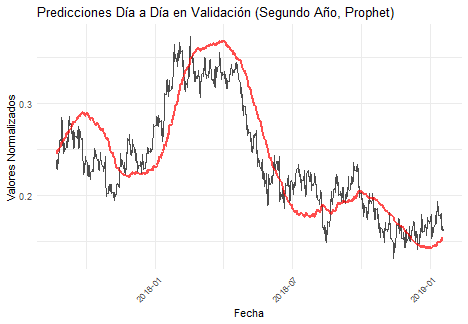
\includegraphics{bookdown_time_series_files/figure-latex/unnamed-chunk-14-1.png}

Estos resultados indican un ajuste razonable del modelo a los datos normalizados, con residuos independientes y métricas de error bajas en el conjunto de entrenamiento, con un MAE de 0,0258 que representan que en promedio las prediciones del modelo se desvian 0,0258 unidades de los valores reales, indicado una desviacion baja.

\section{5. Ajuste del Modelo ARIMA y Evaluación de MAE en Entrenamiento}\label{ajuste-del-modelo-arima-y-evaluaciuxf3n-de-mae-en-entrenamiento}

Ajustamos un modelo ARIMA utilizando los valores \(y\) obtenidos previamente. Usamos auto.arima para seleccionar automáticamente los mejores parámetros.

\begin{verbatim}
## Ajustando modelo ARIMA con auto.arima...
\end{verbatim}

\begin{verbatim}
## 
## Resumen del Modelo ARIMA:
\end{verbatim}

\begin{verbatim}
## Series: train_data$y 
## ARIMA(4,1,0) 
## 
## Coefficients:
##          ar1     ar2      ar3     ar4
##       0.0095  0.0075  -0.0163  0.0121
## s.e.  0.0070  0.0070   0.0070  0.0070
## 
## sigma^2 = 3.647e-05:  log likelihood = 74553.92
## AIC=-149097.8   AICc=-149097.8   BIC=-149058.3
## 
## Training set error measures:
##                         ME        RMSE         MAE  MPE MAPE     MASE
## Training set -2.667179e-07 0.006038687 0.004067731 -Inf  Inf 1.000317
##                       ACF1
## Training set -2.599614e-05
\end{verbatim}

\begin{verbatim}
## 
## MAE en el conjunto de entrenamiento (ARIMA): 0.0041
\end{verbatim}

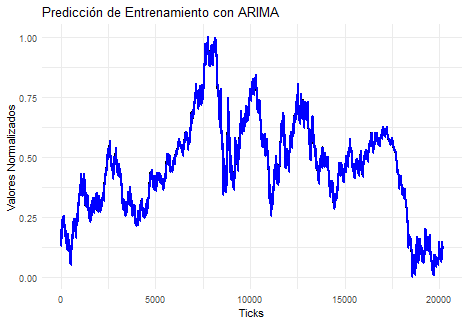
\includegraphics{bookdown_time_series_files/figure-latex/unnamed-chunk-15-1.png}

Como lo habiamos evidenciado en el modelo anterior los resultados indican un ajuste razonable del modelo a los datos normalizados, con residuos independientes y métricas de error bajas en el conjunto de entrenamiento. Sin embargo, la presencia de valores extremos en las métricas como MAPE y MPE (\(-\infty, \infty\)) sugiere posibles problemas en los cálculos debido a la normalización o a valores cercanos a cero.

\section{6. Predicción Día a Día en Validación (ARIMA)}\label{predicciuxf3n-duxeda-a-duxeda-en-validaciuxf3n-arima}

Realizamos la predicion del modelo ARIMA de los ultimo 365 dias con tick 6 (diario)

\begin{verbatim}
## Día 1/365 - MAE del día: 0.0092 - MAE Acumulado: 0.0092Día 2/365 - MAE del día: 0.0044 - MAE Acumulado: 0.0068Día 3/365 - MAE del día: 0.0079 - MAE Acumulado: 0.0071Día 4/365 - MAE del día: 0.0013 - MAE Acumulado: 0.0057Día 5/365 - MAE del día: 0.0026 - MAE Acumulado: 0.0051Día 6/365 - MAE del día: 0.0031 - MAE Acumulado: 0.0047Día 7/365 - MAE del día: 0.0042 - MAE Acumulado: 0.0047Día 8/365 - MAE del día: 0.0051 - MAE Acumulado: 0.0047Día 9/365 - MAE del día: 0.0037 - MAE Acumulado: 0.0046Día 10/365 - MAE del día: 0.0024 - MAE Acumulado: 0.0044Día 11/365 - MAE del día: 0.0042 - MAE Acumulado: 0.0044Día 12/365 - MAE del día: 0.0133 - MAE Acumulado: 0.0051Día 13/365 - MAE del día: 0.0010 - MAE Acumulado: 0.0048Día 14/365 - MAE del día: 0.0045 - MAE Acumulado: 0.0048Día 15/365 - MAE del día: 0.0028 - MAE Acumulado: 0.0046Día 16/365 - MAE del día: 0.0073 - MAE Acumulado: 0.0048Día 17/365 - MAE del día: 0.0051 - MAE Acumulado: 0.0048Día 18/365 - MAE del día: 0.0031 - MAE Acumulado: 0.0047Día 19/365 - MAE del día: 0.0087 - MAE Acumulado: 0.0049Día 20/365 - MAE del día: 0.0073 - MAE Acumulado: 0.0051Día 21/365 - MAE del día: 0.0052 - MAE Acumulado: 0.0051Día 22/365 - MAE del día: 0.0026 - MAE Acumulado: 0.0050Día 23/365 - MAE del día: 0.0067 - MAE Acumulado: 0.0050Día 24/365 - MAE del día: 0.0116 - MAE Acumulado: 0.0053Día 25/365 - MAE del día: 0.0058 - MAE Acumulado: 0.0053Día 26/365 - MAE del día: 0.0087 - MAE Acumulado: 0.0055Día 27/365 - MAE del día: 0.0027 - MAE Acumulado: 0.0054Día 28/365 - MAE del día: 0.0104 - MAE Acumulado: 0.0055Día 29/365 - MAE del día: 0.0038 - MAE Acumulado: 0.0055Día 30/365 - MAE del día: 0.0020 - MAE Acumulado: 0.0054Día 31/365 - MAE del día: 0.0017 - MAE Acumulado: 0.0052Día 32/365 - MAE del día: 0.0068 - MAE Acumulado: 0.0053Día 33/365 - MAE del día: 0.0060 - MAE Acumulado: 0.0053Día 34/365 - MAE del día: 0.0088 - MAE Acumulado: 0.0054Día 35/365 - MAE del día: 0.0034 - MAE Acumulado: 0.0054Día 36/365 - MAE del día: 0.0013 - MAE Acumulado: 0.0052Día 37/365 - MAE del día: 0.0092 - MAE Acumulado: 0.0053Día 38/365 - MAE del día: 0.0037 - MAE Acumulado: 0.0053Día 39/365 - MAE del día: 0.0034 - MAE Acumulado: 0.0053Día 40/365 - MAE del día: 0.0023 - MAE Acumulado: 0.0052Día 41/365 - MAE del día: 0.0075 - MAE Acumulado: 0.0052Día 42/365 - MAE del día: 0.0061 - MAE Acumulado: 0.0053Día 43/365 - MAE del día: 0.0030 - MAE Acumulado: 0.0052Día 44/365 - MAE del día: 0.0090 - MAE Acumulado: 0.0053Día 45/365 - MAE del día: 0.0085 - MAE Acumulado: 0.0054Día 46/365 - MAE del día: 0.0014 - MAE Acumulado: 0.0053Día 47/365 - MAE del día: 0.0100 - MAE Acumulado: 0.0054Día 48/365 - MAE del día: 0.0040 - MAE Acumulado: 0.0053Día 49/365 - MAE del día: 0.0251 - MAE Acumulado: 0.0058Día 50/365 - MAE del día: 0.0021 - MAE Acumulado: 0.0057Día 51/365 - MAE del día: 0.0015 - MAE Acumulado: 0.0056Día 52/365 - MAE del día: 0.0043 - MAE Acumulado: 0.0056Día 53/365 - MAE del día: 0.0114 - MAE Acumulado: 0.0057Día 54/365 - MAE del día: 0.0036 - MAE Acumulado: 0.0056Día 55/365 - MAE del día: 0.0056 - MAE Acumulado: 0.0056Día 56/365 - MAE del día: 0.0119 - MAE Acumulado: 0.0058Día 57/365 - MAE del día: 0.0068 - MAE Acumulado: 0.0058Día 58/365 - MAE del día: 0.0069 - MAE Acumulado: 0.0058Día 59/365 - MAE del día: 0.0047 - MAE Acumulado: 0.0058Día 60/365 - MAE del día: 0.0046 - MAE Acumulado: 0.0058Día 61/365 - MAE del día: 0.0101 - MAE Acumulado: 0.0058Día 62/365 - MAE del día: 0.0093 - MAE Acumulado: 0.0059Día 63/365 - MAE del día: 0.0057 - MAE Acumulado: 0.0059Día 64/365 - MAE del día: 0.0389 - MAE Acumulado: 0.0064Día 65/365 - MAE del día: 0.0073 - MAE Acumulado: 0.0064Día 66/365 - MAE del día: 0.0077 - MAE Acumulado: 0.0064Día 67/365 - MAE del día: 0.0047 - MAE Acumulado: 0.0064Día 68/365 - MAE del día: 0.0017 - MAE Acumulado: 0.0063Día 69/365 - MAE del día: 0.0032 - MAE Acumulado: 0.0063Día 70/365 - MAE del día: 0.0030 - MAE Acumulado: 0.0062Día 71/365 - MAE del día: 0.0065 - MAE Acumulado: 0.0062Día 72/365 - MAE del día: 0.0041 - MAE Acumulado: 0.0062Día 73/365 - MAE del día: 0.0029 - MAE Acumulado: 0.0062Día 74/365 - MAE del día: 0.0034 - MAE Acumulado: 0.0061Día 75/365 - MAE del día: 0.0022 - MAE Acumulado: 0.0061Día 76/365 - MAE del día: 0.0041 - MAE Acumulado: 0.0061Día 77/365 - MAE del día: 0.0035 - MAE Acumulado: 0.0060Día 78/365 - MAE del día: 0.0041 - MAE Acumulado: 0.0060Día 79/365 - MAE del día: 0.0070 - MAE Acumulado: 0.0060Día 80/365 - MAE del día: 0.0027 - MAE Acumulado: 0.0060Día 81/365 - MAE del día: 0.0065 - MAE Acumulado: 0.0060Día 82/365 - MAE del día: 0.0017 - MAE Acumulado: 0.0059Día 83/365 - MAE del día: 0.0030 - MAE Acumulado: 0.0059Día 84/365 - MAE del día: 0.0059 - MAE Acumulado: 0.0059Día 85/365 - MAE del día: 0.0050 - MAE Acumulado: 0.0059Día 86/365 - MAE del día: 0.0017 - MAE Acumulado: 0.0058Día 87/365 - MAE del día: 0.0052 - MAE Acumulado: 0.0058Día 88/365 - MAE del día: 0.0031 - MAE Acumulado: 0.0058Día 89/365 - MAE del día: 0.0106 - MAE Acumulado: 0.0058Día 90/365 - MAE del día: 0.0015 - MAE Acumulado: 0.0058Día 91/365 - MAE del día: 0.0063 - MAE Acumulado: 0.0058Día 92/365 - MAE del día: 0.0065 - MAE Acumulado: 0.0058Día 93/365 - MAE del día: 0.0014 - MAE Acumulado: 0.0058Día 94/365 - MAE del día: 0.0062 - MAE Acumulado: 0.0058Día 95/365 - MAE del día: 0.0012 - MAE Acumulado: 0.0057Día 96/365 - MAE del día: 0.0035 - MAE Acumulado: 0.0057Día 97/365 - MAE del día: 0.0056 - MAE Acumulado: 0.0057Día 98/365 - MAE del día: 0.0063 - MAE Acumulado: 0.0057Día 99/365 - MAE del día: 0.0056 - MAE Acumulado: 0.0057Día 100/365 - MAE del día: 0.0034 - MAE Acumulado: 0.0057Día 101/365 - MAE del día: 0.0145 - MAE Acumulado: 0.0058Día 102/365 - MAE del día: 0.0024 - MAE Acumulado: 0.0057Día 103/365 - MAE del día: 0.0054 - MAE Acumulado: 0.0057Día 104/365 - MAE del día: 0.0058 - MAE Acumulado: 0.0057Día 105/365 - MAE del día: 0.0039 - MAE Acumulado: 0.0057Día 106/365 - MAE del día: 0.0034 - MAE Acumulado: 0.0057Día 107/365 - MAE del día: 0.0056 - MAE Acumulado: 0.0057Día 108/365 - MAE del día: 0.0020 - MAE Acumulado: 0.0057Día 109/365 - MAE del día: 0.0081 - MAE Acumulado: 0.0057Día 110/365 - MAE del día: 0.0023 - MAE Acumulado: 0.0057Día 111/365 - MAE del día: 0.0054 - MAE Acumulado: 0.0056Día 112/365 - MAE del día: 0.0023 - MAE Acumulado: 0.0056Día 113/365 - MAE del día: 0.0046 - MAE Acumulado: 0.0056Día 114/365 - MAE del día: 0.0046 - MAE Acumulado: 0.0056Día 115/365 - MAE del día: 0.0018 - MAE Acumulado: 0.0056Día 116/365 - MAE del día: 0.0104 - MAE Acumulado: 0.0056Día 117/365 - MAE del día: 0.0010 - MAE Acumulado: 0.0056Día 118/365 - MAE del día: 0.0036 - MAE Acumulado: 0.0056Día 119/365 - MAE del día: 0.0046 - MAE Acumulado: 0.0055Día 120/365 - MAE del día: 0.0026 - MAE Acumulado: 0.0055Día 121/365 - MAE del día: 0.0012 - MAE Acumulado: 0.0055Día 122/365 - MAE del día: 0.0035 - MAE Acumulado: 0.0055Día 123/365 - MAE del día: 0.0005 - MAE Acumulado: 0.0054Día 124/365 - MAE del día: 0.0092 - MAE Acumulado: 0.0055Día 125/365 - MAE del día: 0.0026 - MAE Acumulado: 0.0054Día 126/365 - MAE del día: 0.0022 - MAE Acumulado: 0.0054Día 127/365 - MAE del día: 0.0037 - MAE Acumulado: 0.0054Día 128/365 - MAE del día: 0.0042 - MAE Acumulado: 0.0054Día 129/365 - MAE del día: 0.0028 - MAE Acumulado: 0.0054Día 130/365 - MAE del día: 0.0038 - MAE Acumulado: 0.0054Día 131/365 - MAE del día: 0.0041 - MAE Acumulado: 0.0053Día 132/365 - MAE del día: 0.0015 - MAE Acumulado: 0.0053Día 133/365 - MAE del día: 0.0024 - MAE Acumulado: 0.0053Día 134/365 - MAE del día: 0.0045 - MAE Acumulado: 0.0053Día 135/365 - MAE del día: 0.0015 - MAE Acumulado: 0.0053Día 136/365 - MAE del día: 0.0032 - MAE Acumulado: 0.0052Día 137/365 - MAE del día: 0.0014 - MAE Acumulado: 0.0052Día 138/365 - MAE del día: 0.0064 - MAE Acumulado: 0.0052Día 139/365 - MAE del día: 0.0071 - MAE Acumulado: 0.0052Día 140/365 - MAE del día: 0.0074 - MAE Acumulado: 0.0053Día 141/365 - MAE del día: 0.0118 - MAE Acumulado: 0.0053Día 142/365 - MAE del día: 0.0041 - MAE Acumulado: 0.0053Día 143/365 - MAE del día: 0.0054 - MAE Acumulado: 0.0053Día 144/365 - MAE del día: 0.0083 - MAE Acumulado: 0.0053Día 145/365 - MAE del día: 0.0059 - MAE Acumulado: 0.0053Día 146/365 - MAE del día: 0.0040 - MAE Acumulado: 0.0053Día 147/365 - MAE del día: 0.0032 - MAE Acumulado: 0.0053Día 148/365 - MAE del día: 0.0040 - MAE Acumulado: 0.0053Día 149/365 - MAE del día: 0.0055 - MAE Acumulado: 0.0053Día 150/365 - MAE del día: 0.0030 - MAE Acumulado: 0.0053Día 151/365 - MAE del día: 0.0038 - MAE Acumulado: 0.0053Día 152/365 - MAE del día: 0.0075 - MAE Acumulado: 0.0053Día 153/365 - MAE del día: 0.0018 - MAE Acumulado: 0.0053Día 154/365 - MAE del día: 0.0084 - MAE Acumulado: 0.0053Día 155/365 - MAE del día: 0.0020 - MAE Acumulado: 0.0053Día 156/365 - MAE del día: 0.0116 - MAE Acumulado: 0.0053Día 157/365 - MAE del día: 0.0043 - MAE Acumulado: 0.0053Día 158/365 - MAE del día: 0.0050 - MAE Acumulado: 0.0053Día 159/365 - MAE del día: 0.0029 - MAE Acumulado: 0.0053Día 160/365 - MAE del día: 0.0093 - MAE Acumulado: 0.0053Día 161/365 - MAE del día: 0.0017 - MAE Acumulado: 0.0053Día 162/365 - MAE del día: 0.0187 - MAE Acumulado: 0.0054Día 163/365 - MAE del día: 0.0064 - MAE Acumulado: 0.0054Día 164/365 - MAE del día: 0.0062 - MAE Acumulado: 0.0054Día 165/365 - MAE del día: 0.0101 - MAE Acumulado: 0.0054Día 166/365 - MAE del día: 0.0040 - MAE Acumulado: 0.0054Día 167/365 - MAE del día: 0.0040 - MAE Acumulado: 0.0054Día 168/365 - MAE del día: 0.0089 - MAE Acumulado: 0.0054Día 169/365 - MAE del día: 0.0019 - MAE Acumulado: 0.0054Día 170/365 - MAE del día: 0.0042 - MAE Acumulado: 0.0054Día 171/365 - MAE del día: 0.0018 - MAE Acumulado: 0.0054Día 172/365 - MAE del día: 0.0094 - MAE Acumulado: 0.0054Día 173/365 - MAE del día: 0.0034 - MAE Acumulado: 0.0054Día 174/365 - MAE del día: 0.0079 - MAE Acumulado: 0.0054Día 175/365 - MAE del día: 0.0057 - MAE Acumulado: 0.0054Día 176/365 - MAE del día: 0.0046 - MAE Acumulado: 0.0054Día 177/365 - MAE del día: 0.0062 - MAE Acumulado: 0.0054Día 178/365 - MAE del día: 0.0104 - MAE Acumulado: 0.0054Día 179/365 - MAE del día: 0.0055 - MAE Acumulado: 0.0054Día 180/365 - MAE del día: 0.0215 - MAE Acumulado: 0.0055Día 181/365 - MAE del día: 0.0053 - MAE Acumulado: 0.0055Día 182/365 - MAE del día: 0.0037 - MAE Acumulado: 0.0055Día 183/365 - MAE del día: 0.0188 - MAE Acumulado: 0.0056Día 184/365 - MAE del día: 0.0058 - MAE Acumulado: 0.0056Día 185/365 - MAE del día: 0.0104 - MAE Acumulado: 0.0056Día 186/365 - MAE del día: 0.0016 - MAE Acumulado: 0.0056Día 187/365 - MAE del día: 0.0081 - MAE Acumulado: 0.0056Día 188/365 - MAE del día: 0.0220 - MAE Acumulado: 0.0057Día 189/365 - MAE del día: 0.0066 - MAE Acumulado: 0.0057Día 190/365 - MAE del día: 0.0051 - MAE Acumulado: 0.0057Día 191/365 - MAE del día: 0.0056 - MAE Acumulado: 0.0057Día 192/365 - MAE del día: 0.0044 - MAE Acumulado: 0.0057Día 193/365 - MAE del día: 0.0005 - MAE Acumulado: 0.0056Día 194/365 - MAE del día: 0.0012 - MAE Acumulado: 0.0056Día 195/365 - MAE del día: 0.0013 - MAE Acumulado: 0.0056Día 196/365 - MAE del día: 0.0039 - MAE Acumulado: 0.0056Día 197/365 - MAE del día: 0.0088 - MAE Acumulado: 0.0056Día 198/365 - MAE del día: 0.0097 - MAE Acumulado: 0.0056Día 199/365 - MAE del día: 0.0043 - MAE Acumulado: 0.0056Día 200/365 - MAE del día: 0.0084 - MAE Acumulado: 0.0056Día 201/365 - MAE del día: 0.0115 - MAE Acumulado: 0.0057Día 202/365 - MAE del día: 0.0123 - MAE Acumulado: 0.0057Día 203/365 - MAE del día: 0.0084 - MAE Acumulado: 0.0057Día 204/365 - MAE del día: 0.0055 - MAE Acumulado: 0.0057Día 205/365 - MAE del día: 0.0043 - MAE Acumulado: 0.0057Día 206/365 - MAE del día: 0.0035 - MAE Acumulado: 0.0057Día 207/365 - MAE del día: 0.0039 - MAE Acumulado: 0.0057Día 208/365 - MAE del día: 0.0084 - MAE Acumulado: 0.0057Día 209/365 - MAE del día: 0.0035 - MAE Acumulado: 0.0057Día 210/365 - MAE del día: 0.0033 - MAE Acumulado: 0.0057Día 211/365 - MAE del día: 0.0158 - MAE Acumulado: 0.0057Día 212/365 - MAE del día: 0.0062 - MAE Acumulado: 0.0057Día 213/365 - MAE del día: 0.0044 - MAE Acumulado: 0.0057Día 214/365 - MAE del día: 0.0049 - MAE Acumulado: 0.0057Día 215/365 - MAE del día: 0.0026 - MAE Acumulado: 0.0057Día 216/365 - MAE del día: 0.0022 - MAE Acumulado: 0.0057Día 217/365 - MAE del día: 0.0029 - MAE Acumulado: 0.0057Día 218/365 - MAE del día: 0.0099 - MAE Acumulado: 0.0057Día 219/365 - MAE del día: 0.0033 - MAE Acumulado: 0.0057Día 220/365 - MAE del día: 0.0083 - MAE Acumulado: 0.0057Día 221/365 - MAE del día: 0.0116 - MAE Acumulado: 0.0057Día 222/365 - MAE del día: 0.0029 - MAE Acumulado: 0.0057Día 223/365 - MAE del día: 0.0041 - MAE Acumulado: 0.0057Día 224/365 - MAE del día: 0.0029 - MAE Acumulado: 0.0057Día 225/365 - MAE del día: 0.0069 - MAE Acumulado: 0.0057Día 226/365 - MAE del día: 0.0074 - MAE Acumulado: 0.0057Día 227/365 - MAE del día: 0.0029 - MAE Acumulado: 0.0057Día 228/365 - MAE del día: 0.0030 - MAE Acumulado: 0.0057Día 229/365 - MAE del día: 0.0054 - MAE Acumulado: 0.0057Día 230/365 - MAE del día: 0.0034 - MAE Acumulado: 0.0057Día 231/365 - MAE del día: 0.0040 - MAE Acumulado: 0.0056Día 232/365 - MAE del día: 0.0040 - MAE Acumulado: 0.0056Día 233/365 - MAE del día: 0.0081 - MAE Acumulado: 0.0057Día 234/365 - MAE del día: 0.0062 - MAE Acumulado: 0.0057Día 235/365 - MAE del día: 0.0018 - MAE Acumulado: 0.0056Día 236/365 - MAE del día: 0.0075 - MAE Acumulado: 0.0056Día 237/365 - MAE del día: 0.0029 - MAE Acumulado: 0.0056Día 238/365 - MAE del día: 0.0034 - MAE Acumulado: 0.0056Día 239/365 - MAE del día: 0.0026 - MAE Acumulado: 0.0056Día 240/365 - MAE del día: 0.0032 - MAE Acumulado: 0.0056Día 241/365 - MAE del día: 0.0021 - MAE Acumulado: 0.0056Día 242/365 - MAE del día: 0.0051 - MAE Acumulado: 0.0056Día 243/365 - MAE del día: 0.0032 - MAE Acumulado: 0.0056Día 244/365 - MAE del día: 0.0088 - MAE Acumulado: 0.0056Día 245/365 - MAE del día: 0.0029 - MAE Acumulado: 0.0056Día 246/365 - MAE del día: 0.0022 - MAE Acumulado: 0.0056Día 247/365 - MAE del día: 0.0035 - MAE Acumulado: 0.0056Día 248/365 - MAE del día: 0.0056 - MAE Acumulado: 0.0056Día 249/365 - MAE del día: 0.0110 - MAE Acumulado: 0.0056Día 250/365 - MAE del día: 0.0037 - MAE Acumulado: 0.0056Día 251/365 - MAE del día: 0.0021 - MAE Acumulado: 0.0056Día 252/365 - MAE del día: 0.0114 - MAE Acumulado: 0.0056Día 253/365 - MAE del día: 0.0032 - MAE Acumulado: 0.0056Día 254/365 - MAE del día: 0.0033 - MAE Acumulado: 0.0056Día 255/365 - MAE del día: 0.0019 - MAE Acumulado: 0.0055Día 256/365 - MAE del día: 0.0067 - MAE Acumulado: 0.0056Día 257/365 - MAE del día: 0.0012 - MAE Acumulado: 0.0055Día 258/365 - MAE del día: 0.0013 - MAE Acumulado: 0.0055Día 259/365 - MAE del día: 0.0069 - MAE Acumulado: 0.0055Día 260/365 - MAE del día: 0.0034 - MAE Acumulado: 0.0055Día 261/365 - MAE del día: 0.0036 - MAE Acumulado: 0.0055Día 262/365 - MAE del día: 0.0082 - MAE Acumulado: 0.0055Día 263/365 - MAE del día: 0.0074 - MAE Acumulado: 0.0055Día 264/365 - MAE del día: 0.0023 - MAE Acumulado: 0.0055Día 265/365 - MAE del día: 0.0011 - MAE Acumulado: 0.0055Día 266/365 - MAE del día: 0.0014 - MAE Acumulado: 0.0055Día 267/365 - MAE del día: 0.0023 - MAE Acumulado: 0.0055Día 268/365 - MAE del día: 0.0039 - MAE Acumulado: 0.0055Día 269/365 - MAE del día: 0.0051 - MAE Acumulado: 0.0055Día 270/365 - MAE del día: 0.0050 - MAE Acumulado: 0.0055Día 271/365 - MAE del día: 0.0025 - MAE Acumulado: 0.0054Día 272/365 - MAE del día: 0.0044 - MAE Acumulado: 0.0054Día 273/365 - MAE del día: 0.0066 - MAE Acumulado: 0.0054Día 274/365 - MAE del día: 0.0012 - MAE Acumulado: 0.0054Día 275/365 - MAE del día: 0.0034 - MAE Acumulado: 0.0054Día 276/365 - MAE del día: 0.0089 - MAE Acumulado: 0.0054Día 277/365 - MAE del día: 0.0019 - MAE Acumulado: 0.0054Día 278/365 - MAE del día: 0.0039 - MAE Acumulado: 0.0054Día 279/365 - MAE del día: 0.0057 - MAE Acumulado: 0.0054Día 280/365 - MAE del día: 0.0019 - MAE Acumulado: 0.0054Día 281/365 - MAE del día: 0.0055 - MAE Acumulado: 0.0054Día 282/365 - MAE del día: 0.0110 - MAE Acumulado: 0.0054Día 283/365 - MAE del día: 0.0065 - MAE Acumulado: 0.0054Día 284/365 - MAE del día: 0.0064 - MAE Acumulado: 0.0054Día 285/365 - MAE del día: 0.0012 - MAE Acumulado: 0.0054Día 286/365 - MAE del día: 0.0020 - MAE Acumulado: 0.0054Día 287/365 - MAE del día: 0.0046 - MAE Acumulado: 0.0054Día 288/365 - MAE del día: 0.0111 - MAE Acumulado: 0.0054Día 289/365 - MAE del día: 0.0021 - MAE Acumulado: 0.0054Día 290/365 - MAE del día: 0.0061 - MAE Acumulado: 0.0054Día 291/365 - MAE del día: 0.0068 - MAE Acumulado: 0.0054Día 292/365 - MAE del día: 0.0030 - MAE Acumulado: 0.0054Día 293/365 - MAE del día: 0.0018 - MAE Acumulado: 0.0054Día 294/365 - MAE del día: 0.0070 - MAE Acumulado: 0.0054Día 295/365 - MAE del día: 0.0073 - MAE Acumulado: 0.0054Día 296/365 - MAE del día: 0.0116 - MAE Acumulado: 0.0054Día 297/365 - MAE del día: 0.0049 - MAE Acumulado: 0.0054Día 298/365 - MAE del día: 0.0103 - MAE Acumulado: 0.0054Día 299/365 - MAE del día: 0.0093 - MAE Acumulado: 0.0055Día 300/365 - MAE del día: 0.0052 - MAE Acumulado: 0.0055Día 301/365 - MAE del día: 0.0074 - MAE Acumulado: 0.0055Día 302/365 - MAE del día: 0.0024 - MAE Acumulado: 0.0055Día 303/365 - MAE del día: 0.0028 - MAE Acumulado: 0.0054Día 304/365 - MAE del día: 0.0053 - MAE Acumulado: 0.0054Día 305/365 - MAE del día: 0.0024 - MAE Acumulado: 0.0054Día 306/365 - MAE del día: 0.0053 - MAE Acumulado: 0.0054Día 307/365 - MAE del día: 0.0078 - MAE Acumulado: 0.0054Día 308/365 - MAE del día: 0.0032 - MAE Acumulado: 0.0054Día 309/365 - MAE del día: 0.0056 - MAE Acumulado: 0.0054Día 310/365 - MAE del día: 0.0026 - MAE Acumulado: 0.0054Día 311/365 - MAE del día: 0.0017 - MAE Acumulado: 0.0054Día 312/365 - MAE del día: 0.0049 - MAE Acumulado: 0.0054Día 313/365 - MAE del día: 0.0070 - MAE Acumulado: 0.0054Día 314/365 - MAE del día: 0.0020 - MAE Acumulado: 0.0054Día 315/365 - MAE del día: 0.0015 - MAE Acumulado: 0.0054Día 316/365 - MAE del día: 0.0023 - MAE Acumulado: 0.0054Día 317/365 - MAE del día: 0.0038 - MAE Acumulado: 0.0054Día 318/365 - MAE del día: 0.0096 - MAE Acumulado: 0.0054Día 319/365 - MAE del día: 0.0049 - MAE Acumulado: 0.0054Día 320/365 - MAE del día: 0.0041 - MAE Acumulado: 0.0054Día 321/365 - MAE del día: 0.0047 - MAE Acumulado: 0.0054Día 322/365 - MAE del día: 0.0028 - MAE Acumulado: 0.0054Día 323/365 - MAE del día: 0.0014 - MAE Acumulado: 0.0054Día 324/365 - MAE del día: 0.0061 - MAE Acumulado: 0.0054Día 325/365 - MAE del día: 0.0020 - MAE Acumulado: 0.0054Día 326/365 - MAE del día: 0.0183 - MAE Acumulado: 0.0054Día 327/365 - MAE del día: 0.0048 - MAE Acumulado: 0.0054Día 328/365 - MAE del día: 0.0062 - MAE Acumulado: 0.0054Día 329/365 - MAE del día: 0.0055 - MAE Acumulado: 0.0054Día 330/365 - MAE del día: 0.0085 - MAE Acumulado: 0.0054Día 331/365 - MAE del día: 0.0036 - MAE Acumulado: 0.0054Día 332/365 - MAE del día: 0.0031 - MAE Acumulado: 0.0054Día 333/365 - MAE del día: 0.0088 - MAE Acumulado: 0.0054Día 334/365 - MAE del día: 0.0017 - MAE Acumulado: 0.0054Día 335/365 - MAE del día: 0.0009 - MAE Acumulado: 0.0054Día 336/365 - MAE del día: 0.0065 - MAE Acumulado: 0.0054Día 337/365 - MAE del día: 0.0062 - MAE Acumulado: 0.0054Día 338/365 - MAE del día: 0.0045 - MAE Acumulado: 0.0054Día 339/365 - MAE del día: 0.0091 - MAE Acumulado: 0.0054Día 340/365 - MAE del día: 0.0015 - MAE Acumulado: 0.0054Día 341/365 - MAE del día: 0.0106 - MAE Acumulado: 0.0054Día 342/365 - MAE del día: 0.0044 - MAE Acumulado: 0.0054Día 343/365 - MAE del día: 0.0103 - MAE Acumulado: 0.0054Día 344/365 - MAE del día: 0.0026 - MAE Acumulado: 0.0054Día 345/365 - MAE del día: 0.0064 - MAE Acumulado: 0.0054Día 346/365 - MAE del día: 0.0029 - MAE Acumulado: 0.0054Día 347/365 - MAE del día: 0.0065 - MAE Acumulado: 0.0054Día 348/365 - MAE del día: 0.0091 - MAE Acumulado: 0.0054Día 349/365 - MAE del día: 0.0076 - MAE Acumulado: 0.0054Día 350/365 - MAE del día: 0.0084 - MAE Acumulado: 0.0054Día 351/365 - MAE del día: 0.0021 - MAE Acumulado: 0.0054Día 352/365 - MAE del día: 0.0040 - MAE Acumulado: 0.0054Día 353/365 - MAE del día: 0.0032 - MAE Acumulado: 0.0054Día 354/365 - MAE del día: 0.0127 - MAE Acumulado: 0.0054Día 355/365 - MAE del día: 0.0015 - MAE Acumulado: 0.0054Día 356/365 - MAE del día: 0.0065 - MAE Acumulado: 0.0054Día 357/365 - MAE del día: 0.0015 - MAE Acumulado: 0.0054Día 358/365 - MAE del día: 0.0031 - MAE Acumulado: 0.0054Día 359/365 - MAE del día: 0.0063 - MAE Acumulado: 0.0054Día 360/365 - MAE del día: 0.0064 - MAE Acumulado: 0.0054Día 361/365 - MAE del día: 0.0076 - MAE Acumulado: 0.0054Día 362/365 - MAE del día: 0.0045 - MAE Acumulado: 0.0054Día 363/365 - MAE del día: 0.0070 - MAE Acumulado: 0.0054Día 364/365 - MAE del día: 0.0039 - MAE Acumulado: 0.0054Día 365/365 - MAE del día: 0.0072 - MAE Acumulado: 0.0054
\end{verbatim}

\begin{verbatim}
## 
## 
## MAE en validación con ARIMA: 0.0054
\end{verbatim}

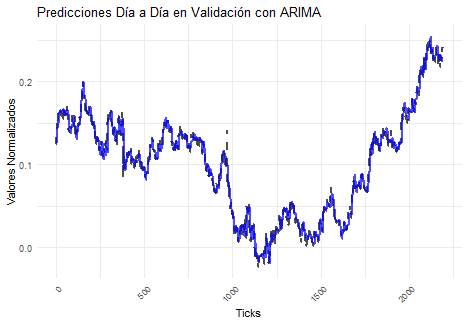
\includegraphics{bookdown_time_series_files/figure-latex/unnamed-chunk-16-1.png}

El error absoluto medio (MAE) del modelo del dia es 0.0072, mientras que en el acumulado es significativamente menor, con un valor de 0.0054. Esto sugiere que el modelo se ajusta bien a los datos de entrenamiento, pero tiene dificultades para generalizar a datos no vistos, indicando un posible sobreajuste o la necesidad de mejorar la capacidad predictiva del modelo.

\section{7. Ajuste y Evaluación del Modelo ETS en Entrenamiento}\label{ajuste-y-evaluaciuxf3n-del-modelo-ets-en-entrenamiento}

En esta etapa se realiza el ajuste y evaluacion del modelo ETS

\begin{verbatim}
## Resumen del Modelo ETS:
\end{verbatim}

\begin{verbatim}
## ETS(A,N,N) 
## 
## Call:
## ets(y = train_data_ts)
## 
##   Smoothing parameters:
##     alpha = 0.9999 
## 
##   Initial states:
##     l = 0.1326 
## 
##   sigma:  0.006
## 
##       AIC      AICc       BIC 
## -6156.589 -6156.588 -6132.849 
## 
## Training set error measures:
##                         ME        RMSE         MAE  MPE MAPE      MASE
## Training set -2.715726e-07 0.006040354 0.004066242 -Inf  Inf 0.1788231
##                     ACF1
## Training set 0.009379616
\end{verbatim}

\begin{verbatim}
## MAE en el conjunto de entrenamiento (ETS): 0.004066242
\end{verbatim}

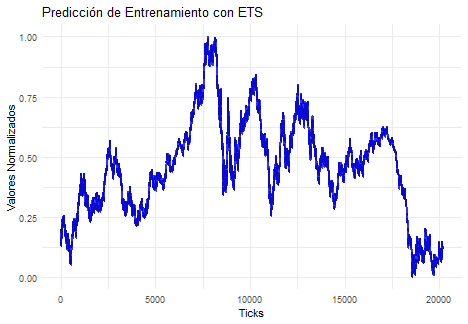
\includegraphics{bookdown_time_series_files/figure-latex/unnamed-chunk-17-1.png}

Los resultados del modelo EST entrenado nos indican un ajuste razonable del modelo a los datos normalizados, con residuos independientes y métricas de error bajas en el conjunto de entrenamiento. Sin embargo, la presencia de valores extremos en las métricas como MAPE y MPE (\(-\infty, \infty\)) indican problemas en la evaluación de la precisión del modelo. Un MAPE infinito sugueire que el modelo no es asertado para el caso, similar a lo observado en el modelo ARIMA

\section{8. Predicciones Día a Día en Validación con ETS}\label{predicciones-duxeda-a-duxeda-en-validaciuxf3n-con-ets}

\begin{verbatim}
## Día 1/365 - MAE del día: 0.0092 - MAE Acumulado: 0.0092Día 2/365 - MAE del día: 0.0044 - MAE Acumulado: 0.0068Día 3/365 - MAE del día: 0.0076 - MAE Acumulado: 0.0071Día 4/365 - MAE del día: 0.0027 - MAE Acumulado: 0.0060Día 5/365 - MAE del día: 0.0026 - MAE Acumulado: 0.0053Día 6/365 - MAE del día: 0.0031 - MAE Acumulado: 0.0049Día 7/365 - MAE del día: 0.0042 - MAE Acumulado: 0.0048Día 8/365 - MAE del día: 0.0051 - MAE Acumulado: 0.0049Día 9/365 - MAE del día: 0.0037 - MAE Acumulado: 0.0047Día 10/365 - MAE del día: 0.0024 - MAE Acumulado: 0.0045Día 11/365 - MAE del día: 0.0042 - MAE Acumulado: 0.0045Día 12/365 - MAE del día: 0.0134 - MAE Acumulado: 0.0052Día 13/365 - MAE del día: 0.0010 - MAE Acumulado: 0.0049Día 14/365 - MAE del día: 0.0044 - MAE Acumulado: 0.0049Día 15/365 - MAE del día: 0.0028 - MAE Acumulado: 0.0047Día 16/365 - MAE del día: 0.0073 - MAE Acumulado: 0.0049Día 17/365 - MAE del día: 0.0051 - MAE Acumulado: 0.0049Día 18/365 - MAE del día: 0.0031 - MAE Acumulado: 0.0048Día 19/365 - MAE del día: 0.0086 - MAE Acumulado: 0.0050Día 20/365 - MAE del día: 0.0056 - MAE Acumulado: 0.0050Día 21/365 - MAE del día: 0.0052 - MAE Acumulado: 0.0050Día 22/365 - MAE del día: 0.0026 - MAE Acumulado: 0.0049Día 23/365 - MAE del día: 0.0068 - MAE Acumulado: 0.0050Día 24/365 - MAE del día: 0.0116 - MAE Acumulado: 0.0053Día 25/365 - MAE del día: 0.0061 - MAE Acumulado: 0.0053Día 26/365 - MAE del día: 0.0046 - MAE Acumulado: 0.0053Día 27/365 - MAE del día: 0.0027 - MAE Acumulado: 0.0052Día 28/365 - MAE del día: 0.0104 - MAE Acumulado: 0.0054Día 29/365 - MAE del día: 0.0037 - MAE Acumulado: 0.0053Día 30/365 - MAE del día: 0.0019 - MAE Acumulado: 0.0052Día 31/365 - MAE del día: 0.0017 - MAE Acumulado: 0.0051Día 32/365 - MAE del día: 0.0068 - MAE Acumulado: 0.0051Día 33/365 - MAE del día: 0.0060 - MAE Acumulado: 0.0052Día 34/365 - MAE del día: 0.0088 - MAE Acumulado: 0.0053Día 35/365 - MAE del día: 0.0034 - MAE Acumulado: 0.0052Día 36/365 - MAE del día: 0.0013 - MAE Acumulado: 0.0051Día 37/365 - MAE del día: 0.0093 - MAE Acumulado: 0.0052Día 38/365 - MAE del día: 0.0036 - MAE Acumulado: 0.0052Día 39/365 - MAE del día: 0.0033 - MAE Acumulado: 0.0051Día 40/365 - MAE del día: 0.0023 - MAE Acumulado: 0.0051Día 41/365 - MAE del día: 0.0090 - MAE Acumulado: 0.0052Día 42/365 - MAE del día: 0.0029 - MAE Acumulado: 0.0051Día 43/365 - MAE del día: 0.0031 - MAE Acumulado: 0.0051Día 44/365 - MAE del día: 0.0081 - MAE Acumulado: 0.0051Día 45/365 - MAE del día: 0.0090 - MAE Acumulado: 0.0052Día 46/365 - MAE del día: 0.0024 - MAE Acumulado: 0.0052Día 47/365 - MAE del día: 0.0080 - MAE Acumulado: 0.0052Día 48/365 - MAE del día: 0.0050 - MAE Acumulado: 0.0052Día 49/365 - MAE del día: 0.0233 - MAE Acumulado: 0.0056Día 50/365 - MAE del día: 0.0022 - MAE Acumulado: 0.0055Día 51/365 - MAE del día: 0.0010 - MAE Acumulado: 0.0054Día 52/365 - MAE del día: 0.0049 - MAE Acumulado: 0.0054Día 53/365 - MAE del día: 0.0114 - MAE Acumulado: 0.0055Día 54/365 - MAE del día: 0.0039 - MAE Acumulado: 0.0055Día 55/365 - MAE del día: 0.0051 - MAE Acumulado: 0.0055Día 56/365 - MAE del día: 0.0119 - MAE Acumulado: 0.0056Día 57/365 - MAE del día: 0.0065 - MAE Acumulado: 0.0056Día 58/365 - MAE del día: 0.0066 - MAE Acumulado: 0.0056Día 59/365 - MAE del día: 0.0046 - MAE Acumulado: 0.0056Día 60/365 - MAE del día: 0.0040 - MAE Acumulado: 0.0056Día 61/365 - MAE del día: 0.0092 - MAE Acumulado: 0.0057Día 62/365 - MAE del día: 0.0098 - MAE Acumulado: 0.0057Día 63/365 - MAE del día: 0.0067 - MAE Acumulado: 0.0057Día 64/365 - MAE del día: 0.0378 - MAE Acumulado: 0.0062Día 65/365 - MAE del día: 0.0028 - MAE Acumulado: 0.0062Día 66/365 - MAE del día: 0.0074 - MAE Acumulado: 0.0062Día 67/365 - MAE del día: 0.0051 - MAE Acumulado: 0.0062Día 68/365 - MAE del día: 0.0020 - MAE Acumulado: 0.0061Día 69/365 - MAE del día: 0.0035 - MAE Acumulado: 0.0061Día 70/365 - MAE del día: 0.0024 - MAE Acumulado: 0.0060Día 71/365 - MAE del día: 0.0072 - MAE Acumulado: 0.0061Día 72/365 - MAE del día: 0.0034 - MAE Acumulado: 0.0060Día 73/365 - MAE del día: 0.0030 - MAE Acumulado: 0.0060Día 74/365 - MAE del día: 0.0038 - MAE Acumulado: 0.0059Día 75/365 - MAE del día: 0.0022 - MAE Acumulado: 0.0059Día 76/365 - MAE del día: 0.0048 - MAE Acumulado: 0.0059Día 77/365 - MAE del día: 0.0038 - MAE Acumulado: 0.0059Día 78/365 - MAE del día: 0.0035 - MAE Acumulado: 0.0058Día 79/365 - MAE del día: 0.0069 - MAE Acumulado: 0.0058Día 80/365 - MAE del día: 0.0020 - MAE Acumulado: 0.0058Día 81/365 - MAE del día: 0.0064 - MAE Acumulado: 0.0058Día 82/365 - MAE del día: 0.0019 - MAE Acumulado: 0.0057Día 83/365 - MAE del día: 0.0030 - MAE Acumulado: 0.0057Día 84/365 - MAE del día: 0.0059 - MAE Acumulado: 0.0057Día 85/365 - MAE del día: 0.0027 - MAE Acumulado: 0.0057Día 86/365 - MAE del día: 0.0017 - MAE Acumulado: 0.0056Día 87/365 - MAE del día: 0.0052 - MAE Acumulado: 0.0056Día 88/365 - MAE del día: 0.0035 - MAE Acumulado: 0.0056Día 89/365 - MAE del día: 0.0107 - MAE Acumulado: 0.0057Día 90/365 - MAE del día: 0.0015 - MAE Acumulado: 0.0056Día 91/365 - MAE del día: 0.0064 - MAE Acumulado: 0.0056Día 92/365 - MAE del día: 0.0065 - MAE Acumulado: 0.0056Día 93/365 - MAE del día: 0.0014 - MAE Acumulado: 0.0056Día 94/365 - MAE del día: 0.0062 - MAE Acumulado: 0.0056Día 95/365 - MAE del día: 0.0012 - MAE Acumulado: 0.0056Día 96/365 - MAE del día: 0.0035 - MAE Acumulado: 0.0055Día 97/365 - MAE del día: 0.0056 - MAE Acumulado: 0.0055Día 98/365 - MAE del día: 0.0062 - MAE Acumulado: 0.0055Día 99/365 - MAE del día: 0.0056 - MAE Acumulado: 0.0055Día 100/365 - MAE del día: 0.0033 - MAE Acumulado: 0.0055Día 101/365 - MAE del día: 0.0145 - MAE Acumulado: 0.0056Día 102/365 - MAE del día: 0.0024 - MAE Acumulado: 0.0056Día 103/365 - MAE del día: 0.0055 - MAE Acumulado: 0.0056Día 104/365 - MAE del día: 0.0043 - MAE Acumulado: 0.0056Día 105/365 - MAE del día: 0.0038 - MAE Acumulado: 0.0055Día 106/365 - MAE del día: 0.0026 - MAE Acumulado: 0.0055Día 107/365 - MAE del día: 0.0041 - MAE Acumulado: 0.0055Día 108/365 - MAE del día: 0.0020 - MAE Acumulado: 0.0055Día 109/365 - MAE del día: 0.0081 - MAE Acumulado: 0.0055Día 110/365 - MAE del día: 0.0023 - MAE Acumulado: 0.0055Día 111/365 - MAE del día: 0.0054 - MAE Acumulado: 0.0055Día 112/365 - MAE del día: 0.0023 - MAE Acumulado: 0.0054Día 113/365 - MAE del día: 0.0046 - MAE Acumulado: 0.0054Día 114/365 - MAE del día: 0.0046 - MAE Acumulado: 0.0054Día 115/365 - MAE del día: 0.0018 - MAE Acumulado: 0.0054Día 116/365 - MAE del día: 0.0103 - MAE Acumulado: 0.0054Día 117/365 - MAE del día: 0.0010 - MAE Acumulado: 0.0054Día 118/365 - MAE del día: 0.0036 - MAE Acumulado: 0.0054Día 119/365 - MAE del día: 0.0046 - MAE Acumulado: 0.0054Día 120/365 - MAE del día: 0.0025 - MAE Acumulado: 0.0054Día 121/365 - MAE del día: 0.0011 - MAE Acumulado: 0.0053Día 122/365 - MAE del día: 0.0033 - MAE Acumulado: 0.0053Día 123/365 - MAE del día: 0.0006 - MAE Acumulado: 0.0053Día 124/365 - MAE del día: 0.0094 - MAE Acumulado: 0.0053Día 125/365 - MAE del día: 0.0026 - MAE Acumulado: 0.0053Día 126/365 - MAE del día: 0.0022 - MAE Acumulado: 0.0052Día 127/365 - MAE del día: 0.0036 - MAE Acumulado: 0.0052Día 128/365 - MAE del día: 0.0042 - MAE Acumulado: 0.0052Día 129/365 - MAE del día: 0.0029 - MAE Acumulado: 0.0052Día 130/365 - MAE del día: 0.0029 - MAE Acumulado: 0.0052Día 131/365 - MAE del día: 0.0041 - MAE Acumulado: 0.0052Día 132/365 - MAE del día: 0.0015 - MAE Acumulado: 0.0052Día 133/365 - MAE del día: 0.0023 - MAE Acumulado: 0.0051Día 134/365 - MAE del día: 0.0045 - MAE Acumulado: 0.0051Día 135/365 - MAE del día: 0.0019 - MAE Acumulado: 0.0051Día 136/365 - MAE del día: 0.0031 - MAE Acumulado: 0.0051Día 137/365 - MAE del día: 0.0013 - MAE Acumulado: 0.0051Día 138/365 - MAE del día: 0.0062 - MAE Acumulado: 0.0051Día 139/365 - MAE del día: 0.0071 - MAE Acumulado: 0.0051Día 140/365 - MAE del día: 0.0078 - MAE Acumulado: 0.0051Día 141/365 - MAE del día: 0.0089 - MAE Acumulado: 0.0051Día 142/365 - MAE del día: 0.0043 - MAE Acumulado: 0.0051Día 143/365 - MAE del día: 0.0055 - MAE Acumulado: 0.0051Día 144/365 - MAE del día: 0.0086 - MAE Acumulado: 0.0052Día 145/365 - MAE del día: 0.0059 - MAE Acumulado: 0.0052Día 146/365 - MAE del día: 0.0037 - MAE Acumulado: 0.0051Día 147/365 - MAE del día: 0.0032 - MAE Acumulado: 0.0051Día 148/365 - MAE del día: 0.0040 - MAE Acumulado: 0.0051Día 149/365 - MAE del día: 0.0069 - MAE Acumulado: 0.0051Día 150/365 - MAE del día: 0.0016 - MAE Acumulado: 0.0051Día 151/365 - MAE del día: 0.0025 - MAE Acumulado: 0.0051Día 152/365 - MAE del día: 0.0074 - MAE Acumulado: 0.0051Día 153/365 - MAE del día: 0.0017 - MAE Acumulado: 0.0051Día 154/365 - MAE del día: 0.0068 - MAE Acumulado: 0.0051Día 155/365 - MAE del día: 0.0020 - MAE Acumulado: 0.0051Día 156/365 - MAE del día: 0.0104 - MAE Acumulado: 0.0051Día 157/365 - MAE del día: 0.0072 - MAE Acumulado: 0.0051Día 158/365 - MAE del día: 0.0020 - MAE Acumulado: 0.0051Día 159/365 - MAE del día: 0.0025 - MAE Acumulado: 0.0051Día 160/365 - MAE del día: 0.0077 - MAE Acumulado: 0.0051Día 161/365 - MAE del día: 0.0016 - MAE Acumulado: 0.0051Día 162/365 - MAE del día: 0.0187 - MAE Acumulado: 0.0052Día 163/365 - MAE del día: 0.0067 - MAE Acumulado: 0.0052Día 164/365 - MAE del día: 0.0060 - MAE Acumulado: 0.0052Día 165/365 - MAE del día: 0.0075 - MAE Acumulado: 0.0052Día 166/365 - MAE del día: 0.0044 - MAE Acumulado: 0.0052Día 167/365 - MAE del día: 0.0053 - MAE Acumulado: 0.0052Día 168/365 - MAE del día: 0.0092 - MAE Acumulado: 0.0052Día 169/365 - MAE del día: 0.0053 - MAE Acumulado: 0.0052Día 170/365 - MAE del día: 0.0037 - MAE Acumulado: 0.0052Día 171/365 - MAE del día: 0.0020 - MAE Acumulado: 0.0052Día 172/365 - MAE del día: 0.0095 - MAE Acumulado: 0.0052Día 173/365 - MAE del día: 0.0040 - MAE Acumulado: 0.0052Día 174/365 - MAE del día: 0.0079 - MAE Acumulado: 0.0052Día 175/365 - MAE del día: 0.0056 - MAE Acumulado: 0.0052Día 176/365 - MAE del día: 0.0046 - MAE Acumulado: 0.0052Día 177/365 - MAE del día: 0.0062 - MAE Acumulado: 0.0052Día 178/365 - MAE del día: 0.0078 - MAE Acumulado: 0.0052Día 179/365 - MAE del día: 0.0056 - MAE Acumulado: 0.0052Día 180/365 - MAE del día: 0.0233 - MAE Acumulado: 0.0053Día 181/365 - MAE del día: 0.0053 - MAE Acumulado: 0.0053Día 182/365 - MAE del día: 0.0012 - MAE Acumulado: 0.0053Día 183/365 - MAE del día: 0.0189 - MAE Acumulado: 0.0054Día 184/365 - MAE del día: 0.0058 - MAE Acumulado: 0.0054Día 185/365 - MAE del día: 0.0104 - MAE Acumulado: 0.0054Día 186/365 - MAE del día: 0.0011 - MAE Acumulado: 0.0054Día 187/365 - MAE del día: 0.0079 - MAE Acumulado: 0.0054Día 188/365 - MAE del día: 0.0120 - MAE Acumulado: 0.0055Día 189/365 - MAE del día: 0.0057 - MAE Acumulado: 0.0055Día 190/365 - MAE del día: 0.0052 - MAE Acumulado: 0.0055Día 191/365 - MAE del día: 0.0039 - MAE Acumulado: 0.0054Día 192/365 - MAE del día: 0.0048 - MAE Acumulado: 0.0054Día 193/365 - MAE del día: 0.0005 - MAE Acumulado: 0.0054Día 194/365 - MAE del día: 0.0014 - MAE Acumulado: 0.0054Día 195/365 - MAE del día: 0.0013 - MAE Acumulado: 0.0054Día 196/365 - MAE del día: 0.0036 - MAE Acumulado: 0.0054Día 197/365 - MAE del día: 0.0088 - MAE Acumulado: 0.0054Día 198/365 - MAE del día: 0.0090 - MAE Acumulado: 0.0054Día 199/365 - MAE del día: 0.0031 - MAE Acumulado: 0.0054Día 200/365 - MAE del día: 0.0084 - MAE Acumulado: 0.0054Día 201/365 - MAE del día: 0.0111 - MAE Acumulado: 0.0054Día 202/365 - MAE del día: 0.0123 - MAE Acumulado: 0.0055Día 203/365 - MAE del día: 0.0084 - MAE Acumulado: 0.0055Día 204/365 - MAE del día: 0.0055 - MAE Acumulado: 0.0055Día 205/365 - MAE del día: 0.0043 - MAE Acumulado: 0.0055Día 206/365 - MAE del día: 0.0035 - MAE Acumulado: 0.0055Día 207/365 - MAE del día: 0.0039 - MAE Acumulado: 0.0055Día 208/365 - MAE del día: 0.0084 - MAE Acumulado: 0.0055Día 209/365 - MAE del día: 0.0035 - MAE Acumulado: 0.0055Día 210/365 - MAE del día: 0.0033 - MAE Acumulado: 0.0055Día 211/365 - MAE del día: 0.0158 - MAE Acumulado: 0.0055Día 212/365 - MAE del día: 0.0062 - MAE Acumulado: 0.0055Día 213/365 - MAE del día: 0.0044 - MAE Acumulado: 0.0055Día 214/365 - MAE del día: 0.0049 - MAE Acumulado: 0.0055Día 215/365 - MAE del día: 0.0026 - MAE Acumulado: 0.0055Día 216/365 - MAE del día: 0.0022 - MAE Acumulado: 0.0055Día 217/365 - MAE del día: 0.0029 - MAE Acumulado: 0.0055Día 218/365 - MAE del día: 0.0099 - MAE Acumulado: 0.0055Día 219/365 - MAE del día: 0.0033 - MAE Acumulado: 0.0055Día 220/365 - MAE del día: 0.0083 - MAE Acumulado: 0.0055Día 221/365 - MAE del día: 0.0116 - MAE Acumulado: 0.0055Día 222/365 - MAE del día: 0.0036 - MAE Acumulado: 0.0055Día 223/365 - MAE del día: 0.0035 - MAE Acumulado: 0.0055Día 224/365 - MAE del día: 0.0029 - MAE Acumulado: 0.0055Día 225/365 - MAE del día: 0.0069 - MAE Acumulado: 0.0055Día 226/365 - MAE del día: 0.0083 - MAE Acumulado: 0.0055Día 227/365 - MAE del día: 0.0027 - MAE Acumulado: 0.0055Día 228/365 - MAE del día: 0.0032 - MAE Acumulado: 0.0055Día 229/365 - MAE del día: 0.0047 - MAE Acumulado: 0.0055Día 230/365 - MAE del día: 0.0030 - MAE Acumulado: 0.0055Día 231/365 - MAE del día: 0.0040 - MAE Acumulado: 0.0055Día 232/365 - MAE del día: 0.0045 - MAE Acumulado: 0.0054Día 233/365 - MAE del día: 0.0051 - MAE Acumulado: 0.0054Día 234/365 - MAE del día: 0.0066 - MAE Acumulado: 0.0055Día 235/365 - MAE del día: 0.0018 - MAE Acumulado: 0.0054Día 236/365 - MAE del día: 0.0065 - MAE Acumulado: 0.0054Día 237/365 - MAE del día: 0.0029 - MAE Acumulado: 0.0054Día 238/365 - MAE del día: 0.0034 - MAE Acumulado: 0.0054Día 239/365 - MAE del día: 0.0026 - MAE Acumulado: 0.0054Día 240/365 - MAE del día: 0.0032 - MAE Acumulado: 0.0054Día 241/365 - MAE del día: 0.0021 - MAE Acumulado: 0.0054Día 242/365 - MAE del día: 0.0051 - MAE Acumulado: 0.0054Día 243/365 - MAE del día: 0.0032 - MAE Acumulado: 0.0054Día 244/365 - MAE del día: 0.0088 - MAE Acumulado: 0.0054Día 245/365 - MAE del día: 0.0031 - MAE Acumulado: 0.0054Día 246/365 - MAE del día: 0.0022 - MAE Acumulado: 0.0054Día 247/365 - MAE del día: 0.0035 - MAE Acumulado: 0.0054Día 248/365 - MAE del día: 0.0056 - MAE Acumulado: 0.0054Día 249/365 - MAE del día: 0.0111 - MAE Acumulado: 0.0054Día 250/365 - MAE del día: 0.0037 - MAE Acumulado: 0.0054Día 251/365 - MAE del día: 0.0047 - MAE Acumulado: 0.0054Día 252/365 - MAE del día: 0.0093 - MAE Acumulado: 0.0054Día 253/365 - MAE del día: 0.0032 - MAE Acumulado: 0.0054Día 254/365 - MAE del día: 0.0033 - MAE Acumulado: 0.0054Día 255/365 - MAE del día: 0.0019 - MAE Acumulado: 0.0054Día 256/365 - MAE del día: 0.0068 - MAE Acumulado: 0.0054Día 257/365 - MAE del día: 0.0012 - MAE Acumulado: 0.0054Día 258/365 - MAE del día: 0.0013 - MAE Acumulado: 0.0053Día 259/365 - MAE del día: 0.0068 - MAE Acumulado: 0.0053Día 260/365 - MAE del día: 0.0034 - MAE Acumulado: 0.0053Día 261/365 - MAE del día: 0.0036 - MAE Acumulado: 0.0053Día 262/365 - MAE del día: 0.0082 - MAE Acumulado: 0.0053Día 263/365 - MAE del día: 0.0074 - MAE Acumulado: 0.0053Día 264/365 - MAE del día: 0.0023 - MAE Acumulado: 0.0053Día 265/365 - MAE del día: 0.0011 - MAE Acumulado: 0.0053Día 266/365 - MAE del día: 0.0014 - MAE Acumulado: 0.0053Día 267/365 - MAE del día: 0.0023 - MAE Acumulado: 0.0053Día 268/365 - MAE del día: 0.0039 - MAE Acumulado: 0.0053Día 269/365 - MAE del día: 0.0062 - MAE Acumulado: 0.0053Día 270/365 - MAE del día: 0.0023 - MAE Acumulado: 0.0053Día 271/365 - MAE del día: 0.0025 - MAE Acumulado: 0.0053Día 272/365 - MAE del día: 0.0044 - MAE Acumulado: 0.0053Día 273/365 - MAE del día: 0.0066 - MAE Acumulado: 0.0053Día 274/365 - MAE del día: 0.0012 - MAE Acumulado: 0.0053Día 275/365 - MAE del día: 0.0035 - MAE Acumulado: 0.0052Día 276/365 - MAE del día: 0.0089 - MAE Acumulado: 0.0053Día 277/365 - MAE del día: 0.0019 - MAE Acumulado: 0.0052Día 278/365 - MAE del día: 0.0040 - MAE Acumulado: 0.0052Día 279/365 - MAE del día: 0.0057 - MAE Acumulado: 0.0052Día 280/365 - MAE del día: 0.0019 - MAE Acumulado: 0.0052Día 281/365 - MAE del día: 0.0086 - MAE Acumulado: 0.0052Día 282/365 - MAE del día: 0.0066 - MAE Acumulado: 0.0053Día 283/365 - MAE del día: 0.0038 - MAE Acumulado: 0.0052Día 284/365 - MAE del día: 0.0064 - MAE Acumulado: 0.0052Día 285/365 - MAE del día: 0.0012 - MAE Acumulado: 0.0052Día 286/365 - MAE del día: 0.0020 - MAE Acumulado: 0.0052Día 287/365 - MAE del día: 0.0046 - MAE Acumulado: 0.0052Día 288/365 - MAE del día: 0.0111 - MAE Acumulado: 0.0052Día 289/365 - MAE del día: 0.0021 - MAE Acumulado: 0.0052Día 290/365 - MAE del día: 0.0047 - MAE Acumulado: 0.0052Día 291/365 - MAE del día: 0.0053 - MAE Acumulado: 0.0052Día 292/365 - MAE del día: 0.0035 - MAE Acumulado: 0.0052Día 293/365 - MAE del día: 0.0018 - MAE Acumulado: 0.0052Día 294/365 - MAE del día: 0.0070 - MAE Acumulado: 0.0052Día 295/365 - MAE del día: 0.0073 - MAE Acumulado: 0.0052Día 296/365 - MAE del día: 0.0142 - MAE Acumulado: 0.0053Día 297/365 - MAE del día: 0.0068 - MAE Acumulado: 0.0053Día 298/365 - MAE del día: 0.0082 - MAE Acumulado: 0.0053Día 299/365 - MAE del día: 0.0113 - MAE Acumulado: 0.0053Día 300/365 - MAE del día: 0.0070 - MAE Acumulado: 0.0053Día 301/365 - MAE del día: 0.0056 - MAE Acumulado: 0.0053Día 302/365 - MAE del día: 0.0029 - MAE Acumulado: 0.0053Día 303/365 - MAE del día: 0.0028 - MAE Acumulado: 0.0053Día 304/365 - MAE del día: 0.0041 - MAE Acumulado: 0.0053Día 305/365 - MAE del día: 0.0024 - MAE Acumulado: 0.0053Día 306/365 - MAE del día: 0.0053 - MAE Acumulado: 0.0053Día 307/365 - MAE del día: 0.0078 - MAE Acumulado: 0.0053Día 308/365 - MAE del día: 0.0032 - MAE Acumulado: 0.0053Día 309/365 - MAE del día: 0.0072 - MAE Acumulado: 0.0053Día 310/365 - MAE del día: 0.0026 - MAE Acumulado: 0.0053Día 311/365 - MAE del día: 0.0017 - MAE Acumulado: 0.0053Día 312/365 - MAE del día: 0.0032 - MAE Acumulado: 0.0052Día 313/365 - MAE del día: 0.0053 - MAE Acumulado: 0.0052Día 314/365 - MAE del día: 0.0028 - MAE Acumulado: 0.0052Día 315/365 - MAE del día: 0.0016 - MAE Acumulado: 0.0052Día 316/365 - MAE del día: 0.0021 - MAE Acumulado: 0.0052Día 317/365 - MAE del día: 0.0039 - MAE Acumulado: 0.0052Día 318/365 - MAE del día: 0.0097 - MAE Acumulado: 0.0052Día 319/365 - MAE del día: 0.0050 - MAE Acumulado: 0.0052Día 320/365 - MAE del día: 0.0041 - MAE Acumulado: 0.0052Día 321/365 - MAE del día: 0.0021 - MAE Acumulado: 0.0052Día 322/365 - MAE del día: 0.0029 - MAE Acumulado: 0.0052Día 323/365 - MAE del día: 0.0015 - MAE Acumulado: 0.0052Día 324/365 - MAE del día: 0.0061 - MAE Acumulado: 0.0052Día 325/365 - MAE del día: 0.0020 - MAE Acumulado: 0.0052Día 326/365 - MAE del día: 0.0183 - MAE Acumulado: 0.0052Día 327/365 - MAE del día: 0.0048 - MAE Acumulado: 0.0052Día 328/365 - MAE del día: 0.0062 - MAE Acumulado: 0.0052Día 329/365 - MAE del día: 0.0025 - MAE Acumulado: 0.0052Día 330/365 - MAE del día: 0.0076 - MAE Acumulado: 0.0052Día 331/365 - MAE del día: 0.0035 - MAE Acumulado: 0.0052Día 332/365 - MAE del día: 0.0031 - MAE Acumulado: 0.0052Día 333/365 - MAE del día: 0.0088 - MAE Acumulado: 0.0052Día 334/365 - MAE del día: 0.0017 - MAE Acumulado: 0.0052Día 335/365 - MAE del día: 0.0009 - MAE Acumulado: 0.0052Día 336/365 - MAE del día: 0.0065 - MAE Acumulado: 0.0052Día 337/365 - MAE del día: 0.0062 - MAE Acumulado: 0.0052Día 338/365 - MAE del día: 0.0045 - MAE Acumulado: 0.0052Día 339/365 - MAE del día: 0.0078 - MAE Acumulado: 0.0052Día 340/365 - MAE del día: 0.0019 - MAE Acumulado: 0.0052Día 341/365 - MAE del día: 0.0109 - MAE Acumulado: 0.0052Día 342/365 - MAE del día: 0.0057 - MAE Acumulado: 0.0052Día 343/365 - MAE del día: 0.0102 - MAE Acumulado: 0.0052Día 344/365 - MAE del día: 0.0048 - MAE Acumulado: 0.0052Día 345/365 - MAE del día: 0.0064 - MAE Acumulado: 0.0052Día 346/365 - MAE del día: 0.0036 - MAE Acumulado: 0.0052Día 347/365 - MAE del día: 0.0066 - MAE Acumulado: 0.0052Día 348/365 - MAE del día: 0.0068 - MAE Acumulado: 0.0052Día 349/365 - MAE del día: 0.0087 - MAE Acumulado: 0.0053Día 350/365 - MAE del día: 0.0084 - MAE Acumulado: 0.0053Día 351/365 - MAE del día: 0.0024 - MAE Acumulado: 0.0053Día 352/365 - MAE del día: 0.0056 - MAE Acumulado: 0.0053Día 353/365 - MAE del día: 0.0021 - MAE Acumulado: 0.0052Día 354/365 - MAE del día: 0.0113 - MAE Acumulado: 0.0053Día 355/365 - MAE del día: 0.0015 - MAE Acumulado: 0.0053Día 356/365 - MAE del día: 0.0056 - MAE Acumulado: 0.0053Día 357/365 - MAE del día: 0.0015 - MAE Acumulado: 0.0052Día 358/365 - MAE del día: 0.0031 - MAE Acumulado: 0.0052Día 359/365 - MAE del día: 0.0063 - MAE Acumulado: 0.0052Día 360/365 - MAE del día: 0.0043 - MAE Acumulado: 0.0052Día 361/365 - MAE del día: 0.0076 - MAE Acumulado: 0.0052Día 362/365 - MAE del día: 0.0045 - MAE Acumulado: 0.0052Día 363/365 - MAE del día: 0.0070 - MAE Acumulado: 0.0053Día 364/365 - MAE del día: 0.0039 - MAE Acumulado: 0.0052Día 365/365 - MAE del día: 0.0072 - MAE Acumulado: 0.0053
\end{verbatim}

\begin{verbatim}
## 
## 
## MAE en validación con ETS: 0.0053
\end{verbatim}

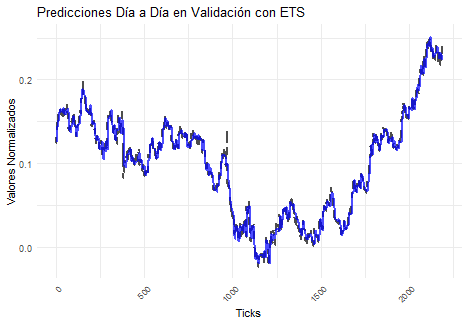
\includegraphics{bookdown_time_series_files/figure-latex/unnamed-chunk-18-1.png}

El error absoluto medio (MAE) del modelo del dia es 0.0072 idicando un valor bajo que indica precision en la proyeccion diaria, sin embargo el MAE acumulado es significativamente menor, con un valor de 0.0053 idicando que hay un mayor ajuste en la seria acumulada y mayor presicion. Pero al igual que con el modelo anterior el modelo se ajusta bien a los datos de entrenamiento, pero tiene dificultades para generalizar a datos no vistos.

\section{9. Tabla Comparativa de MAE}\label{tabla-comparativa-de-mae}

\begin{table}
\centering
\caption{\label{tab:unnamed-chunk-19}Comparación de MAE entre Modelos}
\centering
\fontsize{14}{16}\selectfont
\begin{tabular}[t]{>{}l|>{}c|>{}c}
\hline
\multicolumn{1}{c|}{ } & \multicolumn{2}{c}{Error Absoluto Medio} \\
\cline{2-3}
\cellcolor{black}{\textcolor{white}{\textbf{Modelo}}} & \cellcolor{black}{\textcolor{white}{\textbf{MAE Entrenamiento}}} & \cellcolor{black}{\textcolor{white}{\textbf{MAE Validación}}}\\
\hline
\textcolor{black}{\textbf{ARIMA}} & \textcolor{blue}{0.0041} & \textcolor{blue}{0.0054}\\
\hline
\textcolor{black}{\textbf{ETS}} & \textcolor{blue}{0.0041} & \textcolor{blue}{0.0053}\\
\hline
\textcolor{black}{\textbf{Prophet}} & \textcolor{blue}{0.0097} & \textcolor{blue}{0.0258}\\
\hline
\end{tabular}
\end{table}

\section{10. Discusión}\label{discusiuxf3n}

En la evaluación comparativa de los modelos, \textbf{ETS} y \textbf{ARIMA} demostraron ser las técnicas más robustas, con MAE en validación de \textbf{0.0053} y \textbf{0.0054}, respectivamente. Estos resultados destacan la capacidad de ambos modelos para generalizar sobre los datos de validación, capturando patrones temporales relevantes. En contraste, \textbf{Prophet}, aunque intuitivo y versátil, presentó un desempeño inferior con un MAE de validación de \textbf{0.0258}, probablemente debido a su incapacidad para modelar eficientemente los patrones intradía específicos de esta serie temporal.

Una posible explicación para el desempeño superior de ETS radica en su diseño para manejar automáticamente estacionalidades y tendencias, mientras que ARIMA requirió preprocesamiento adicional (diferenciación) para garantizar la estacionariedad de los datos. Por otro lado, el pobre rendimiento de Prophet sugiere que su parametrización predeterminada podría no ser adecuada para series temporales con alta granularidad y comportamiento intradía.

Es importante considerar que el MAE es solo una métrica de error absoluto. Para aplicaciones prácticas, otros factores como la interpretabilidad del modelo, los costos computacionales y la facilidad de implementación deben formar parte del proceso de selección. Adicionalmente, los datos utilizados se limitaron a una frecuencia fija de 4 horas; explorar otras periodicidades o incorporar características externas podría impactar significativamente los resultados.

\begin{center}\rule{0.5\linewidth}{0.5pt}\end{center}

\section{\texorpdfstring{\textbf{Sección 11: Conclusiones}}{Sección 11: Conclusiones}}\label{secciuxf3n-11-conclusiones}

\begin{enumerate}
\def\labelenumi{\arabic{enumi}.}
\item
  \textbf{Mejor Modelo:} El \textbf{modelo ETS} fue el más efectivo para este conjunto de datos, logrando el MAE más bajo en validación (\textbf{0.0053}), lo que lo convierte en la opción recomendada para aplicaciones prácticas en predicción de series temporales intradía.
\item
  \textbf{Desempeño de ARIMA:} Aunque ligeramente superado por ETS, ARIMA mostró un rendimiento consistente, con un \textbf{MAE en validación de 0.0054}, destacándose como una alternativa confiable para series temporales que requieren análisis más detallados de componentes estocásticos.
\item
  \textbf{Limitación de Prophet:} Con un MAE en validación de \textbf{0.0258}, Prophet no logró capturar adecuadamente los patrones intradía. Ajustes adicionales en sus parámetros o su combinación con otras técnicas podrían ser necesarios para mejorar su rendimiento en escenarios similares.
\end{enumerate}

  \bibliography{book.bib,packages.bib}

\end{document}
